% arara: pdflatex: {synctex: yes, action: nonstopmode}
% arara: pdflatex 
% arara: bibtex  !!On each included chapter seperately!!
% arara: pdflatex
% arara: pdflatex
% arara: nomencl
% arara: pdflatex: {synctex: yes, action: nonstopmode}

%\documentclass[a4crop]{ntnuthesis} 
\documentclass{ntnuthesis}  
\usepackage{amsmath} %equations and spacings
\usepackage{lipsum} 
\usepackage{graphicx}
\usepackage[small,bf]{caption}
\usepackage[labelformat=simple]{subcaption}
\usepackage{pdfpages}
\usepackage{amssymb}
%\usepackage{amsfonts}
\usepackage{array}
\usepackage{multirow}
\usepackage{algorithmic}
\usepackage{algorithm}
\usepackage{pdflscape}
\renewcommand\thesubfigure{(\alph{subfigure})} % see subcaption doc

%Abbreviations or Acronyms
%\usepackage[intoc]{nomencl}
\usepackage{nomencl}
\renewcommand{\nomname}{List of Abbreviations}
\makenomenclature

%Bibliography
%\usepackage{url}
%\usepackage{natbib}%\usepackage[sectionbib]{natbib} DEN ITAN COMMENTED
\usepackage{chapterbib}
%\bibpunct[:]{(}{)}{;}{a}{}{,} %citation structure DEN ITAN COMMENTED
%\bibpunct{(}{)}{,}{a}{}{;} 
%\bibpunct{[}{]}{,}{a}{}{;}
%\bibpunct{(}{)}{;}{a}{}{,} % to follow the A&A style
%\usepackage{chapterbib}
\usepackage{hyperref}
%for blank pages:
\usepackage{afterpage}
%\hypersetup{colorlinks=true,citecolor=blue}
\hypersetup{colorlinks=true,citecolor=blue,linkcolor=blue,urlcolor=blue}

%To change box color around the links and citations, you have these other options :
%\hypersetup{citebordercolor=Violet,filebordercolor=Red,linkbordercolor=Blue}

\newcommand{\cmt}[1]{}%inline comment
  
%tabularx
\usepackage{tabularx}
\usepackage{tabulary}
\usepackage{longtable} %table on several pages
\usepackage{booktabs}
\usepackage{multirow}
\usepackage{dcolumn}

%graphics
\usepackage{epstopdf} %support for eps.
\DeclareGraphicsExtensions{.eps,.ps,.pdf,.png,.jpg}
\usepackage{float} % figure placing [H]

%landscape Option
\usepackage{lscape} %Left down
%usepackage{pdflscape} %Left up)

%spaces under sections
\usepackage[compact]{titlesec}
%\titlespacing{\section}{0pt}{*0}{*0}
%\titlespacing{\subsection}{0pt}{*0}{*0}
%\titlespacing{\subsubsection}{0pt}{*0}{*0}
\titlespacing*{\section}
{0pt}{5.5ex plus 1ex minus .2ex}{4.3ex plus .2ex}
\titlespacing*{\subsection}
{0pt}{5.5ex plus 1ex minus .2ex}{4.3ex plus .2ex}


\usepackage[draft]{todonotes}   % notes showed (JJUNJU)
% Select what to do with command \comment:  
% \newcommand{\comment}[1]{}  %comment not showed
\newcommand{\comment}[1]
{\par {\bfseries \color{red} #1 \par}} %comment showed

%Section Numbering and TOC depth
\setcounter{secnumdepth}{2}
\setcounter{tocdepth}{3}

%chapter biblio
\usepackage{chapterbib}

%To generate list of symbols
\newcommand{\addsymbol}[3]{%
  \symboldisplay{#1}{#2}\\%
  \setelem{#3}{#1}
}
\newcommand{\symboldisplay}[2]{%
  $#1$ \parbox{5in}{\dotfill #2}%
  %$#1$ \parbox{5in}{ #2}%
}
%\def\setelem#1{\expandafter\def\csname myarray(#1)\endcsname}
\def\setelem#1{\expandafter\gdef\csname myarray(#1)\endcsname}
\def\dispsymbol#1{\csname myarray(#1)\endcsname} 


%START!!
%Titles
\title{Exploration of energy \\efficient memory \\organizations exploiting \\data variable based \\system scenarios}
%\subtitle{Subtitle of the thesis here}
\author{Iason Filippopoulos}

\def \thesisAuthor{Iason Filippopoulos}

%\degreetype{PhD}
\faculty{Faculty of Information Technology, Mathematics and Electrical Engineering \\ Department of Electronics and Telecommunications \\}
\department{Catholic University of Leuven \\ Department of Electrical Engineering}
\copyrightnotice{All rights reserved}
\isbnprinted{}
\isbnelectronic{}
\serialnumber{}
\setyear{2015}
\setmonth{September}

\begin{document}

\frontmatter
\maketitle

%<<byman
%% Configuration of the header strings for the frontmatter pages.
\fancyhead[RO]{{\footnotesize\rightmark}\hspace{1em}\thepage}
\setcounter{tocdepth}{2}
\fancyhead[LE]{\thepage\hspace{1em}\footnotesize{\leftmark}}
\fancyhead[RE,LO]{}
\fancyhead[RO]{{\footnotesize\rightmark}\hspace{1em}\thepage}
%byman>>

\vspace*{\fill}
\addcontentsline{toc}{section}{Abstract}
\section*{\hspace*{\fill} Abstract \hspace*{\fill}}

Modern embedded systems are capable of performing a wide range of tasks and their popularity is increasing in many different application domains.
The recent progress on the semiconductor processing technology greatly improves the performance of the embedded systems, due to the increased number of transistors on a single chip.
The continuous performance improvement increases the possibilities for new embedded system designs.
However, many embedded systems rely on a battery source, which puts a significant limitation on their lifetime and usage.
The management of the energy consumption is the key factor towards increasing the lifetime of an embedded system relying on a battery source.
%%Assuming that the development in the battery technology will follow the current trend, embedded systems should improve their energy efficiency based on the system design.
A typical embedded system includes one or more processing elements (CPUs, GPUs, embedded processors etc.), a memory subsystem (cache, scratchpad, flash, etc.) and application specific hardware (antennas, sensors, etc.). 
The memory subsystem is a significant contribution to the overall energy based on the study of existing and proposed embedded systems.
Especially for applications that are data intensive, the memory architecture may have the highest energy footprint of the whole embedded system.

In this thesis, we focus on the design of energy efficient memory architectures for embedded systems.
A hardware/software co-design methodology is proposed for the reduction of the energy consumption on the memory subsystem. 
The  methodology exploits variations in memory needs during the lifetime of an application in order to optimize energy usage. 
The different resource requirements, that change dynamically at run-time, are organized into groups to efficiently handle a very large exploration space.
Apart from the development of the methodology, an extended memory model is included in this work. 
The memory models is based on existing state-of-the-art memories, available from industry and academia.
In addition, the impact of the technology scaling is studied and the effectiveness of the proposed methodology is analyzed for the future memory architectures.
We also investigate the combination of the developed methodology with known code transformation techniques, specifically data interleaving.
The proposed design methodology aims to be compatible with the already available code optimization techniques.
%We further extend the evaluation of the memory design methodology using a test-case wireless system.
%The proposed reconfigurable memory subsystem is studied in a dynamic platform with several reconfiguration options that combine the memory and the processing elements.
\vspace*{\fill}
\afterpage{\null\newpage}
\newpage


\vspace*{\fill}
\addcontentsline{toc}{section}{Preface}
\section*{\Huge Preface }
\bigskip
\bigskip
This doctoral thesis was submitted to the Norwegian University of Science and Technology (NTNU) in partial fulfillment of the requirements for the degree philosophiae doctor (PhD). 
The thesis is a part of a dual PhD program between NTNU and the Catholic University of Leuven (K. U. Leuven), in cooperation with Interuniversity Microelectronics Center (IMEC).
The work herein was performed at the Department of Electronics and Telecommunications, NTNU and the Department of Electrical Engineering, KU Leuven.
The work was performed under the supervision of Professor Per Gunnar Kjeldsberg and Professor Francky Catthoor.

\bigskip
\bigskip

\addcontentsline{toc}{section}{Acknowledgements}
\section*{Acknowledgements}

\bigskip

I would like to thank my supervisors Prof. Per Gunnar Kjeldsberg and Prof. Francky Catthoor for their support and advise through the long process that eventually became this thesis. 
I also extend my gratitude to my co-supervisor Prof. Sverre Hendseth for providing encouragement and positive attitude all these years.

I would also like to thank Mladen for sharing both his direct and thought-provoking opinions and office space with me.
Furthermore, I thank Elena and Yahya for our great co-operation and their patience on the evaluation meetings.
I was lucky to meet great co-workers at NTNU and IMEC that offered their help. 

Finally, I would like to thank my family and friends for their support. 

\bigskip

\begin{flushright}
Iason Filippopoulos \\
September 2015
\end{flushright}

\vspace*{\fill}

%TOC
\tableofcontents
%\addcontentsline{toc}{chapter}{Contents}
\cleardoublepage

\listoftables	
\addcontentsline{toc}{chapter}{List of Tables}
\cleardoublepage

\listoffigures	
\addcontentsline{toc}{chapter}{List of Figures}
\cleardoublepage

%Abbreviations
\newpage
%\thispagestyle{empty}
\printnomenclature
\cleardoublepage

%Symbols
\newpage
\chapter*{List of Symbols\hfill} 
\addcontentsline{toc}{chapter}{List of Symbols}
\begin{flushleft}
%	\input{symbols}
\end{flushleft}

\mainmatter

\cleardoublepage
%Chapters
\chapter{Introduction}
\label{intro}


\section{Embedded Systems and Energy Consumption - what is our general goal}

\section{Data Intensive Applications - what is our general goal}

\section{Brief summary of current way of tackling and what has not been addressed here}

\section{Problem Statement}

\section{Proposed Solution}

\section{Thesis Outline - what is covered in which paper} 
\chapter{Background} %use enough space up to 15-20 pages
\label{background}

\section{Scratch-pad Memory Architectures - related work incl}

\section{System Scenarios - all the literature with focus on the ones related}
	- vs. use case
	- pareto

\section{DTSE}
	-


\chapter{Methodology}
\label{method}
%make a consistent story about how the papers are connetcted

\section{System Scenario Platform}

\subsection{Target memory platform architecture}

\subsection{Memory models}

\subsection{Technology scaling}

\section{Data variable based memory-aware system scenario methodology}

\subsection{Interleaving exploration based on data variables}

\subsection{Design-time profiling based on data variables}

\subsection{Design-time system scenario identification based on data variables}

\subsection{Run-time system scenario detection and switching based on data variables}




\chapter{Research Results and Contributions}
\label{research}

\section{Contribution A: Memory-Aware Methodology Development}

\section{Contribution B: System Scenarios on Memory and PEs}

\section{Contribution C: Integrated Interleaving and Data-to-Memory Mapping}

\section{Contribution D: Interconnection Cost Modeling and Scaling}

\section{Paper A.I - Abstract - My contribution}

\section{Paper A.II}

\section{Paper A.III}

\section{Paper B.I}

\section{Paper C.I}

\section{Paper D.I}
\chapter{Conclusions}
\label{conclusions}

   

%\bibliographystyle{plain}
%\bibliography{reference} 

%<<byman
%% Configuration of the header strings for the Appendices
%\renewcommand{\chaptermark}[1]{%
%  \markboth{\MakeUppercase{\appendixname\ \thechapter}}%
%  {\MakeUppercase{#1}}
%}
%\fancyhead[RE,LO]{}
%
%\appendix
%byman>>
\appendix
%
%\title{Memory-Aware System Scenario Approach \\ Energy Impact}
%\author{\IEEEauthorblockN{Iason Filippopoulos\IEEEauthorrefmark{1},
%Francky Catthoor\IEEEauthorrefmark{2},
%Per Gunnar Kjeldsberg\IEEEauthorrefmark{1}, 
%Elena Hammari\IEEEauthorrefmark{1} and
%Jos Huisken\IEEEauthorrefmark{3}}
%\IEEEauthorblockA{\IEEEauthorrefmark{1}Department of Electronics and Telecommunications\\
%Norwegian University of Science and Technology,
%Trondheim, Norway\\ Email: iason.filippopoulos@iet.ntnu.no}
%\IEEEauthorblockA{\IEEEauthorrefmark{2}IMEC, Kapeldreef 75, 3000 Leuven, Belgium\\}
%\IEEEauthorblockA{\IEEEauthorrefmark{3}Holst Centre / IMEC Netherlands, High Tech Campus 31, Eindhoven, The Netherlands\\}}
%
%% make the title area


\chapter{Energy Impact of Memory-Aware System Scenario Approach}
\label{norchip}

\begin{center}
Iason Filippopoulos, Francky Catthoor, Per Gunnar Kjeldsberg, \\ Elena Hammari and Jos Huisken
\\
IEEE NORCHIP conference
\\
2012
\end{center}
\afterpage{\null\newpage}
\newpage

\vspace*{\fill}
\phantomsection
\section*{\hspace*{\fill} Abstract \hspace*{\fill}}
\addcontentsline{toc}{section}{Abstract}
System scenario methodologies propose the use of different scenarios, e.g., different platform configurations, in order to exploit variations in computational and memory needs during the lifetime of an application. In this paper several extensions are proposed for a system scenario based methodology with a focus on improving memory organisation. The conventional methodology targets mostly execution time while this work aims at including memory costs into the exploration. The effectiveness of the proposed extensions is demonstrated and tested using two real applications, which are dynamic and suitable for execution on modern embedded systems. Reductions in memory energy consumption of 40 to 70\% is shown.
\vspace*{\fill}
\afterpage{\null\newpage}
\newpage

\section{Introduction}
\label{sec:introduction}

Modern embedded systems are becoming more and more powerful as the semiconductor processing technique keep increasing the number of transistors on a single chip. Consequentially, demanding applications, such as medical signal processing and streaming applications, can be executed on these devices \cite{narasinga}. On the other hand, the desired performance has to be delivered with the minimum power consumption due to limited amount of power offered in mobile devices \cite{tcm}. System scenario methodologies propose the use of different platform configurations in order to exploit variations in computational and memory needs often seen during the lifetime of such applications \cite{tcm}. A platform can, e.g., be configured through frequency/voltage scaling or turning certain processing units on or off. In this work a reconfigurable memory platform is employed in order to study the effectiveness of a memory-aware system scenario methodology.

As shown in \cite{Gonzalez1996} memory contributes around 40\% to the overall power consumption in general purpose systems. Especially for embedded systems, the memory subsystem accounts for up to 50\% of the overall energy consumption \cite{Che09} and the cycle-accurate simulator presented in \cite{Ben99} estimates that the energy expenditures in the memory subsystem range from 35\% up to 65\% for different architectures. According to \cite{tcm}, conventional allocation and mapping of data done by regular compilers is suboptimal. Performance loss is caused by stalls for fetching data and data conflicts for different tasks, due to the limited size of memory and the competition between tasks. In addition, modern applications exhibit more and more dynamism. This gives a strong motivation for study and optimization of memory organisation in embedded devices with strongly dynamic application behaviour.

This paper is organized as follows. Section~\ref{sec:related} surveys related work on system level exploration and on system scenario methodologies. Section~\ref{sec:methodology} presents the chosen methodology and our novel extensions to make it applicable in a memory organisation study. In Section~\ref{sec:platform} the target platform is described while the demonstrator applications are presented in Section~\ref{sec:applications}. Results of applying the described methodology to the targeted applications are shown in Section~\ref{sec:results}, while conclusions are drawn in Section~\ref{sec:conclusion}. The main contribution of the current work is the proposal of extensions to the existing system scenario methodology, in order to take into account memory costs while performing the design exploration.  

\section{Related Work and Contribution Discussion}
\label{sec:related}

Many papers have focused on memory related optimisations, also in the presence of a partitioned and distributed memory organisation with memory blocks of different sizes (e.g. \cite{Ben00b}, \cite{Ben00c}, \cite{Mac02}, \cite{Pgk01}). However, they do not incorporate sufficient support for very dynamically behaving application codes. System scenarios allow to alleviate this bottleneck and to handle such dynamic behaviour. An overview of work on system scenario methodologies and their application are presented in \cite{Gheorghita2007}. So far memory organisation is rarely considered and not fully analysed. Furthermore, the majority of the published work focus on control variables for scenario prediction and selection. They can take a relatively small set of different values that can be fully explored. However, the use of data variables \cite{Elena2010} is required for these tasks by many dynamic systems with value ranges that make full exploration impossible. 

Authors in \cite{Pal06} present a technique to optimise memory accesses for input data dependent applications by duplicating and optimising the code for different execution paths of a control flow graph (CFG) \nomenclature{CFG}{control flow graph}. One path or a group of paths in a CFG form a scenario and its memory accesses are optimized using global loop transformations (GLT) \nomenclature{GLT}{global loop transformations}. Apart from if-statement evaluations that define different execution paths, they extend their technique to include while loops with variable trip count in \cite{Pal06b}. A heuristic to perform efficient grouping of execution paths for scenario creation is analysed in \cite{Pal07}. However, our work extends the existing solutions towards exploiting the presence of a distributed memory organisation with reconfiguration possibilities.

Reconfigurable hardware for embedded systems, including the memory architecture, is a topic of active research. An extensive overview of current approaches is found in \cite{Garcia}. The approach presented in this paper differentiates by focusing on the data-to-memory partitioning aspects in the presence of a platform with dynamically configurable memory blocks. 

\section{Extended System Scenario Methodology}
\label{sec:methodology}

The system scenario methodology is based on the observation that the workload of most systems varies significantly during their lifetime due to dynamic variation of computational and memory needs in the application code. Most of the existing design methods define the worst case execution time (WCET) \nomenclature{WCET}{worst case execution time} of the most demanding task and tune the system in order to meet its needs \cite{tcm}. Obviously, this approach leads to wasted time and memory area for tasks with lower execution time and memory requirements, since those tasks could meet their needs using fewer resources and consequentially consuming less energy. 

In contrast, designing with scenarios is workload adaptive and offers different configurations of the platform and the freedom of switching to the most efficient scenario at run-time. In contrast to use case scenario approaches in which scenarios are generated based on a user's behaviour, the system scenario methodology focuses on behaviour of the system to generate scenarios. A system scenario is a configuration of the system that combines similar run-time situations (RTSs). An RTS consists of a running instance of a task and its corresponding cost (e.g. energy consumption) and one complete run of the application on the target platform represents a sequence of RTSs \cite{Elena2010}. The system is configured to meet the cost requirements of an RTS by choosing the appropriate scenario, which is the one that satisfies the requirements using minimal power.

In the following subsections, the different steps of the system scenario methodology is outlined, with emphasis on the new extensions that make it possible to take memory into account. 

\subsection{General description of system scenario methodology}

The scenario methodology follows a two stage exploration, namely design-time and run-time stages, as described in \cite{Gheorghita2007}. The two stage exploration is chosen because it reduces run-time overhead while preserving an important degree of freedom for run-time configuration \cite{tcm}. In more detail, the application is analysed at design-time and different execution paths and variations in processing and memory demands are identified. This procedure, which is time consuming and as a result can be performed only during the design phase, will result in a grey-box model representation of the application. The grey-box model hides all static and deterministic parts of the application, by providing only related costs for those, and keeps parts of the application code that are non-deterministic available to the system designer \cite{graybox}. This way, more focus can be given to parts of the application that have impact on the cost variations so that different execution decisions can be studied. Those different options are made available to the system designer and each decision could be either fixed at design time or forwarded for dynamic evaluation at run-time.

\subsection{Design-time Profiling}

Application profiling is performed at design-time and consists of an analysis of the target application during its lifetime and for a wide range of inputs. The analysis focuses on execution time for a reference processor in the conventional system scenario methodology, but in our case the cost will be memory size. This cost metric is chosen, because several applications allocate and deallocate memory space during their execution. Also, data reuse behavior and decisions made by the system designer about the size of sets of data to be copied to different units in the memory hierarchy (i.e., copy-candidates \cite{dtse}) strongly influences the memory size. Energy consumption and access time of a memory unit is affected by its size \cite{patterson}. Together with access pattern information, the memory size is hence an important metric.

The flow of the profiling stage is depicted in Fig.~\ref{fig:profilingA} and consists of running the application code with suitable input data often found in a database, in order to produce profiling results. This reveals parts of the application code with high memory activity and with varying memory access intensity, which possibly depends on input data. Because of this behaviour, a static study of the application code alone is insufficient since the target applications for this methodology have non-deterministic behaviour that is driven by input. Choosing an extensive and accurate database is vital and will heavily influence and steer the designer's decisions in later steps.

\begin{figure}[!t]
\centering
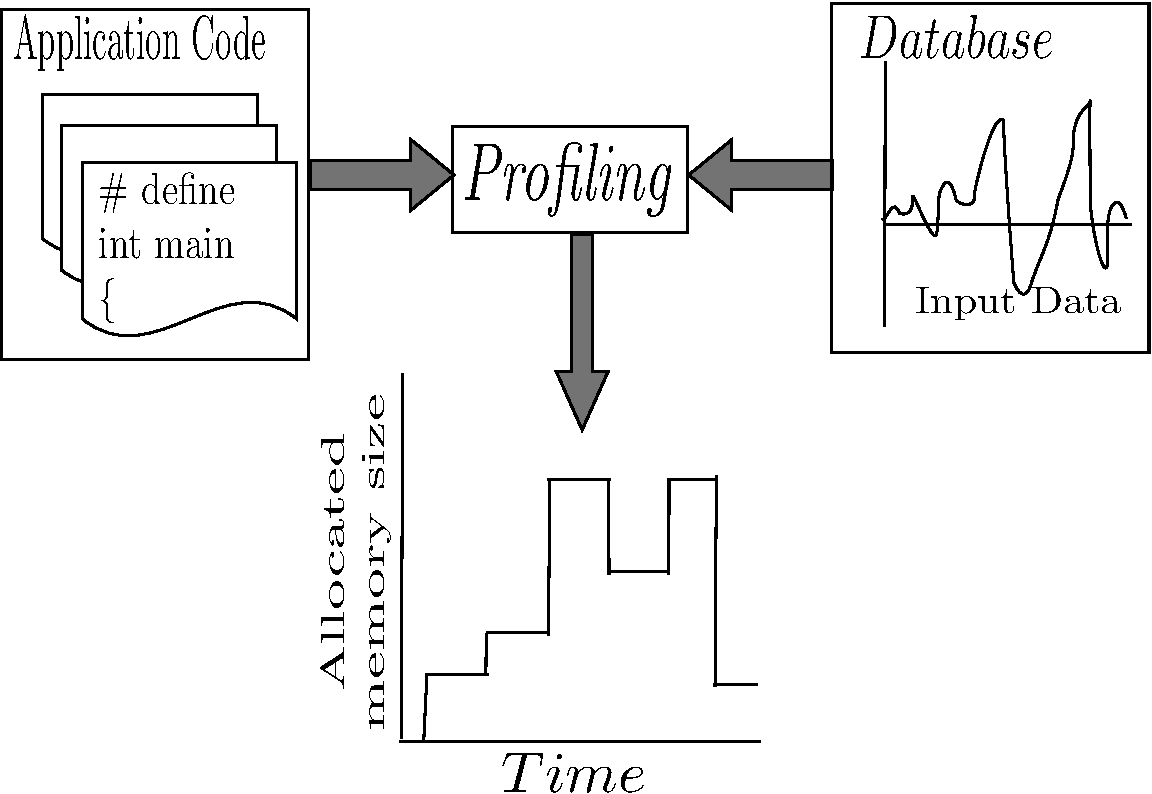
\includegraphics[width=0.8\textwidth]{A/profiling_v2-eps-converted-to.pdf}
\caption{Profiling results based on application code and input data.}
\label{fig:profilingA}
\end{figure}

Given code and database as inputs, profiling will show memory usage during execution time by running the application using the whole database as an input. Results provided to the designer include complete information about allocated memory size values together with the number of occurrences and duration for each of these memory size values. Moreover, correlation between input data values and the resulting memory behaviour can possibly be observed. This information is forwarded to the next stage.

There are several ways that profiling can be performed. Current program monitoring software cannot offer the needed level of detail. Debuggers and memory tools, such as Valgrind \cite{Valgrind}, or direct hard-coded profiling are preferable methods, because of their higher accuracy.

\subsection{Design-time Scenario Identification and Prediction}

Scenario generation is also performed during design time and is the procedure of clustering profiled information into groups with similar characteristics. More precisely, cost points are clustered in groups based on their distance in cost axis and the frequency of their occurrence. Clustering is necessary, because it will be extremely costly to have a different scenario for every possible situation. Switching cost, which is the cost of switching platform to another configuration, for example by turning a memory to retention state, grows with the number of scenarios, because more scenarios result in more frequent switching. In addition, the runtime manager becomes more complex with an increasing number of scenarios.

As shown in Fig.~\ref{fig:clusteringA}, using the information available after application profiling, situations with similar platform needs will be organised in a common scenario. This is known as clustering of RTSs \cite{Gheorghita2007}. This is a rational choice, because two instances with similar platform needs have similar memory energy consumption. The energy gain of having two dedicated scenarios is small and normally outweighed by switching costs if organized in different scenarios. In this example, clustering results in three different scenario areas (Fig.~\ref{fig:clusteringA}) and the execution scenario sequence is 1(lower), 2(middle), 3(top), 2, 3 and 1. Also, the frequency of occurrence of each instance is an important factor in scenario generation. Instances with higher frequencies normally have their dedicated scenario, to allow higher optimization, while less common instances can be clustered together in a less optimal scenario. 

In order to generate scenarios that can be implemented in realistic memory organisations, a detailed library with memory components is needed. The library should contain a variety of memory models, including different technologies and sizes, and is used to calculate scenario costs. In this work the component library is based on memory models published in \cite{Artes2011}.

\begin{figure}[!t]
\centering
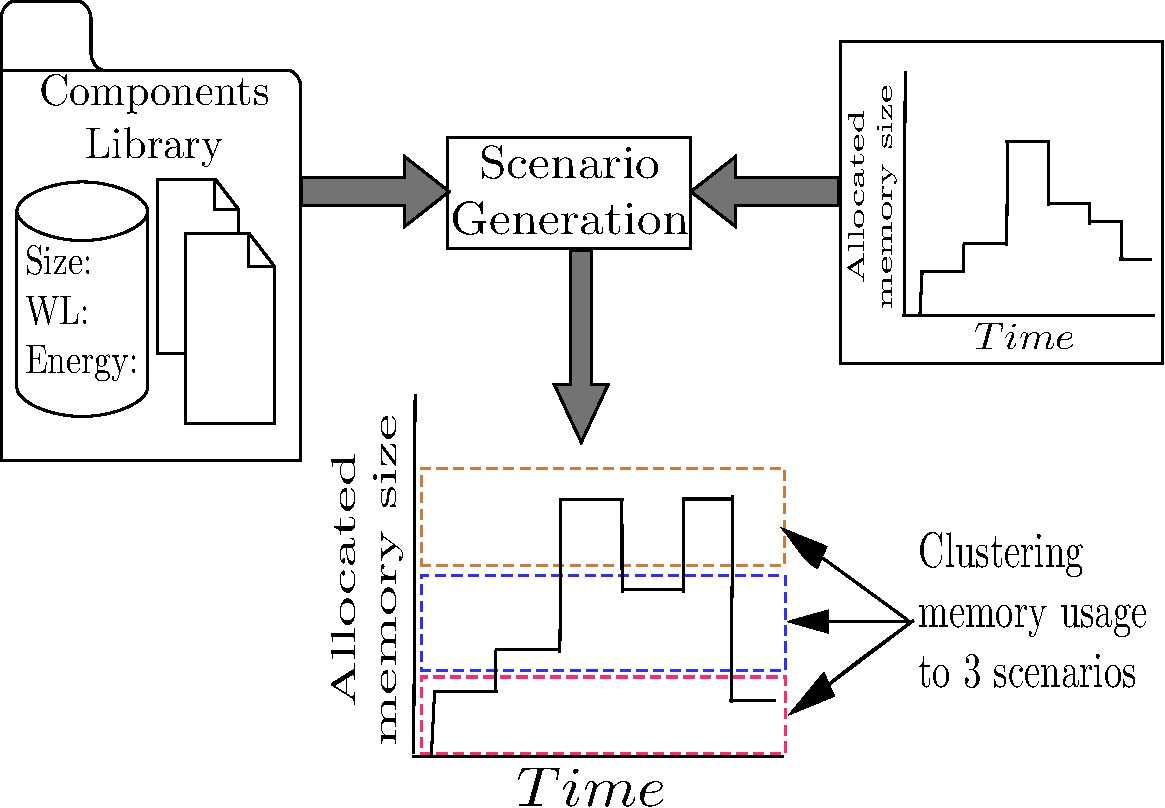
\includegraphics[width=0.8\textwidth]{A/clustering_v2-eps-converted-to.pdf}
\caption{Scenario generation based on profiling information and memory models.}
\label{fig:clusteringA}
\end{figure}

The design-time scenario prediction phase consists of determination of the variables that define the active scenario. This can be achieved by careful study of the application code, combined with the application's data input. In our case the grey-box model reveals only the code parts that will influence memory usage, so that variables deciding memory space changes can be identified. An example of this is a non static variable that influences the number of iterations for a loop that performs one memory allocation at each iteration. Moreover, the designer should look for a correlation between input values and the corresponding cost. This information will be useful in the following steps of the methodology \cite{tcm}.

\subsection{Run-time Identification, Detection, and Switching}

After profiling and scenario generation at design-time, all the necessary information needed for run-time management is available. The run-time manager monitors the current values of prediction variables selected in the previous design time step. Based on this, prediction of the next active scenario is performed  \cite{tcm}. 

Switching decisions will be taken at run-time by the run-time manager. The switching phase consists of all platform configuration decisions that can be made at run-time, e.g., frequency/voltage scaling, turning on/off a memory unit, and remapping of data on memory units. Switching takes place when the switching cost is lower than the energy gains achieved by switching. In more detail, the run-time manager compares the memory energy consumption of executing the next task in the current active scenario with the energy consumption of execution with the optimal scenario. If the difference is greater than the switching cost, then scenario switching is performed \cite{tcm}. Switching costs are defined by the platform and include all memory energy penalties for run-time reconfigurations of the platform, e.g., extra energy needed to change state of a memory unit.

\section{Target Platform}
\label{sec:platform}

Selection of target platform is an important aspect of the memory-aware system scenario methodology. The key feature needed in the platform architecture is the ability to realize different scenarios generated by the methodology. Execution of different scenarios then leads to different energy costs, as each configuration of the platform results in a specific memory energy consumption. In the conventional system scenario methodology several platform reconfiguration options have been studied \cite{Gheorghita2007} with dynamic voltage/frequency scaling (DVFS) most used \cite{dvfs}. By using DVFS techniques, one can change the frequency of the processing element and its supply voltage and energy consumption accordingly. For a memory aware scenario methodology there are multiple ways that memory reconfiguration can be performed. E.g., data can be mapped to different memory units according to size and access frequency, memory units can be turned on or off, or DVFS can be used to allow exactly the access frequency currently needed. 

\begin{figure}[!t]
\centering
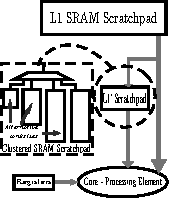
\includegraphics[width=0.8\textwidth]{A/platform_v10-eps-converted-to.pdf}
\caption{Target platform with focus on memory organisation.}
\label{fig:platformA}
\end{figure}

In this paper we have selected a relatively conventional reconfigurable architecture template that is suitable for implementing system scenarios as shown in Fig.~\ref{fig:platformA}. This dynamic memory organisation is based on memory prototypes presented in \cite{Artes2011}, and consists of two software controlled SRAM scratchpad memories, L1 and L1', and a processing element with its registers. For simplicity it is assumed that all data needed during execution is available in the L1 scratchpad memory without any time penalties even when large background memories are used. This assumption is reasonable for the kind of applications that are generally executed in embedded systems and can, e.g., be achieved through prefetching. The methodology is in general not restricted to this assumption, however, and can handle more complex hierarchical memory architectures, also including regular caches. Registers are used to save currently used elements, and between the registers and the L1 scratchpad a much smaller L1' scratchpad is introduced. This is a clustered memory that consists of four memory banks that support three different states (on, off and retention modes) \cite{Artes2011}. 

The memory energy consumption for every access in the clustered scratchpad memory is calculated based on the current situation of the platform as shown in Fig.~\ref{fig:platformA}. The leakage energy estimation is also provided in \cite{Artes2011} and is included in our study. In Tab.~\ref{tab:leakage} the leakage and wake up costs for all different operation modes are presented. The leakage in L1' is small compared to L1 and constant, thus the effect in the results is minimal.

\begin{table}[!t]
\centering
\caption{Energy costs per second and access for a reference memory bank (size: 120 bytes, technology: 90nm) in clustered L1' memory }
\label{tab:leakage}
\begin{tabular}{|c|c|c|c|c|c|c|c|}
\hline 
Modes & Leakage [J] & Wake up [J] & Access [J]\\ 
\hline 
On & $351,86 \times 10 ^{-6}$ & - & -  \\ 
\hline 
Off & $ 4,73 \times 10 ^{-6}$ & $ 2,77 \times 10 ^{-12}$ & -\\ 
\hline 
Retention & $ 97,33 \times 10 ^{-6}$ & $ 2,2 \times 10 ^{-12}$ & -\\ 
\hline 
DFF synch & - & - & $ 0.227 \times 10 ^{-6}$\\ 
\hline
DFF asynch & - & - & $ 2.18 \times 10 ^{-6}$\\ 
\hline 
Nand2 & - & - & $ 0.334 \times 10 ^{-6}$\\ 
\hline
\end{tabular}      
\end{table}

The memory energy consumption per read access is given by Equation ~\ref{eq:energyA}, which is provided by the memory models in \cite{Artes2011}.    
\begin{multline}
Read \: energy = (size \: of \: bank) \times (DFF \: sync)+ \\ + \dfrac{bank \: lines}{log2} \times DFF \: async + 4 \times size \times Nand2 
\label{eq:energyA}
\end{multline}
The cost of accessing the clustered scratchpad organisation is a function of the overall size of the cluster and the size of the specific bank being accessed. In addition, there is a contribution in energy consumption per access added by the flip-flops and the gates needed for the correct operation of the L1' memory organisation.
 
\section{Application Benchmarks}
\label{sec:applications}

The extended methodology will be tested on two representative real life applications that differentiate significantly from each other and cover different domains of applications. The first one is a computational intensive application, in which the code is dominated by loops with dynamic bounds determined by results calculated inside the loop. The second has a more static execution path, but its memory footprint is dynamically defined by the input data. Ideal applications, that can most benefit from memory-aware system scenario methodology, are applications that have dynamic behaviour in memory organisation utilization during their execution. That required dynamism could be produced by several code characteristics, covering a wide range of potential application domains for the proposed methodology.

\subsection{Epileptic Seizure Predictor}

An epileptic seizure predictor algorithm developed at Arizona State University (ASU) \cite{Iasemidis2005} is chosen as a benchmark, along with a database with measurements performed on real patients, also provided by ASU. Up to now the algorithm has only been used in clinical environments using PCs, although it would be very helpful for patients as an embedded device, as part of outpatient care. Dynamic input data dependent behaviour is identified in the algorithm and memory traces for execution of three different input samples are presented in Fig.~\ref{fig:eegprof}. For each data sample a loop is iterated 168 times. Depending on the input data sample, different memory elements are accessed in each iteration. Note that even though the element accessing for all three samples are drawn together in the figure, only one set of memory elements are accessed for each data sample and only one data sample is processed at a time. Because of the nature of the EEG \nomenclature{EEG}{electroencephalogram} signal used for the epileptic seizure prediction the benchmark has variables with a very wide range of potential values. The memory usage is heavily influenced by these input values. For demonstration purposes our study focuses on the parts of the prediction algorithm that is most dynamic. In \cite{Elena2010} the algorithm is split in thread nodes and dynamic behaviour affecting execution time is identified. The data reuse size for each sample in Fig.~\ref{fig:eegprof} contains all the elements with data reuse factor greater than 1, i.e., are read more than once. They should be saved in L1'. For example, elements in index range from roughly 3300 to 7200 for sample 1 form an approximately 3900$ \times $(element size bytes) L1' memory size requirement. These elements are read for the first time between loop iteration 0 and 50 and are also re-read later during the sample's lifetime between loop iteration 120 and 170. In Fig.~\ref{fig:eegprof} these memory elements are included in the red rectangle. The exact L1' sizes needed for processing of sample 1, 2, and 3 are 3899, 2646, and 3780, respectively.

\begin{figure}[!t]
\centering
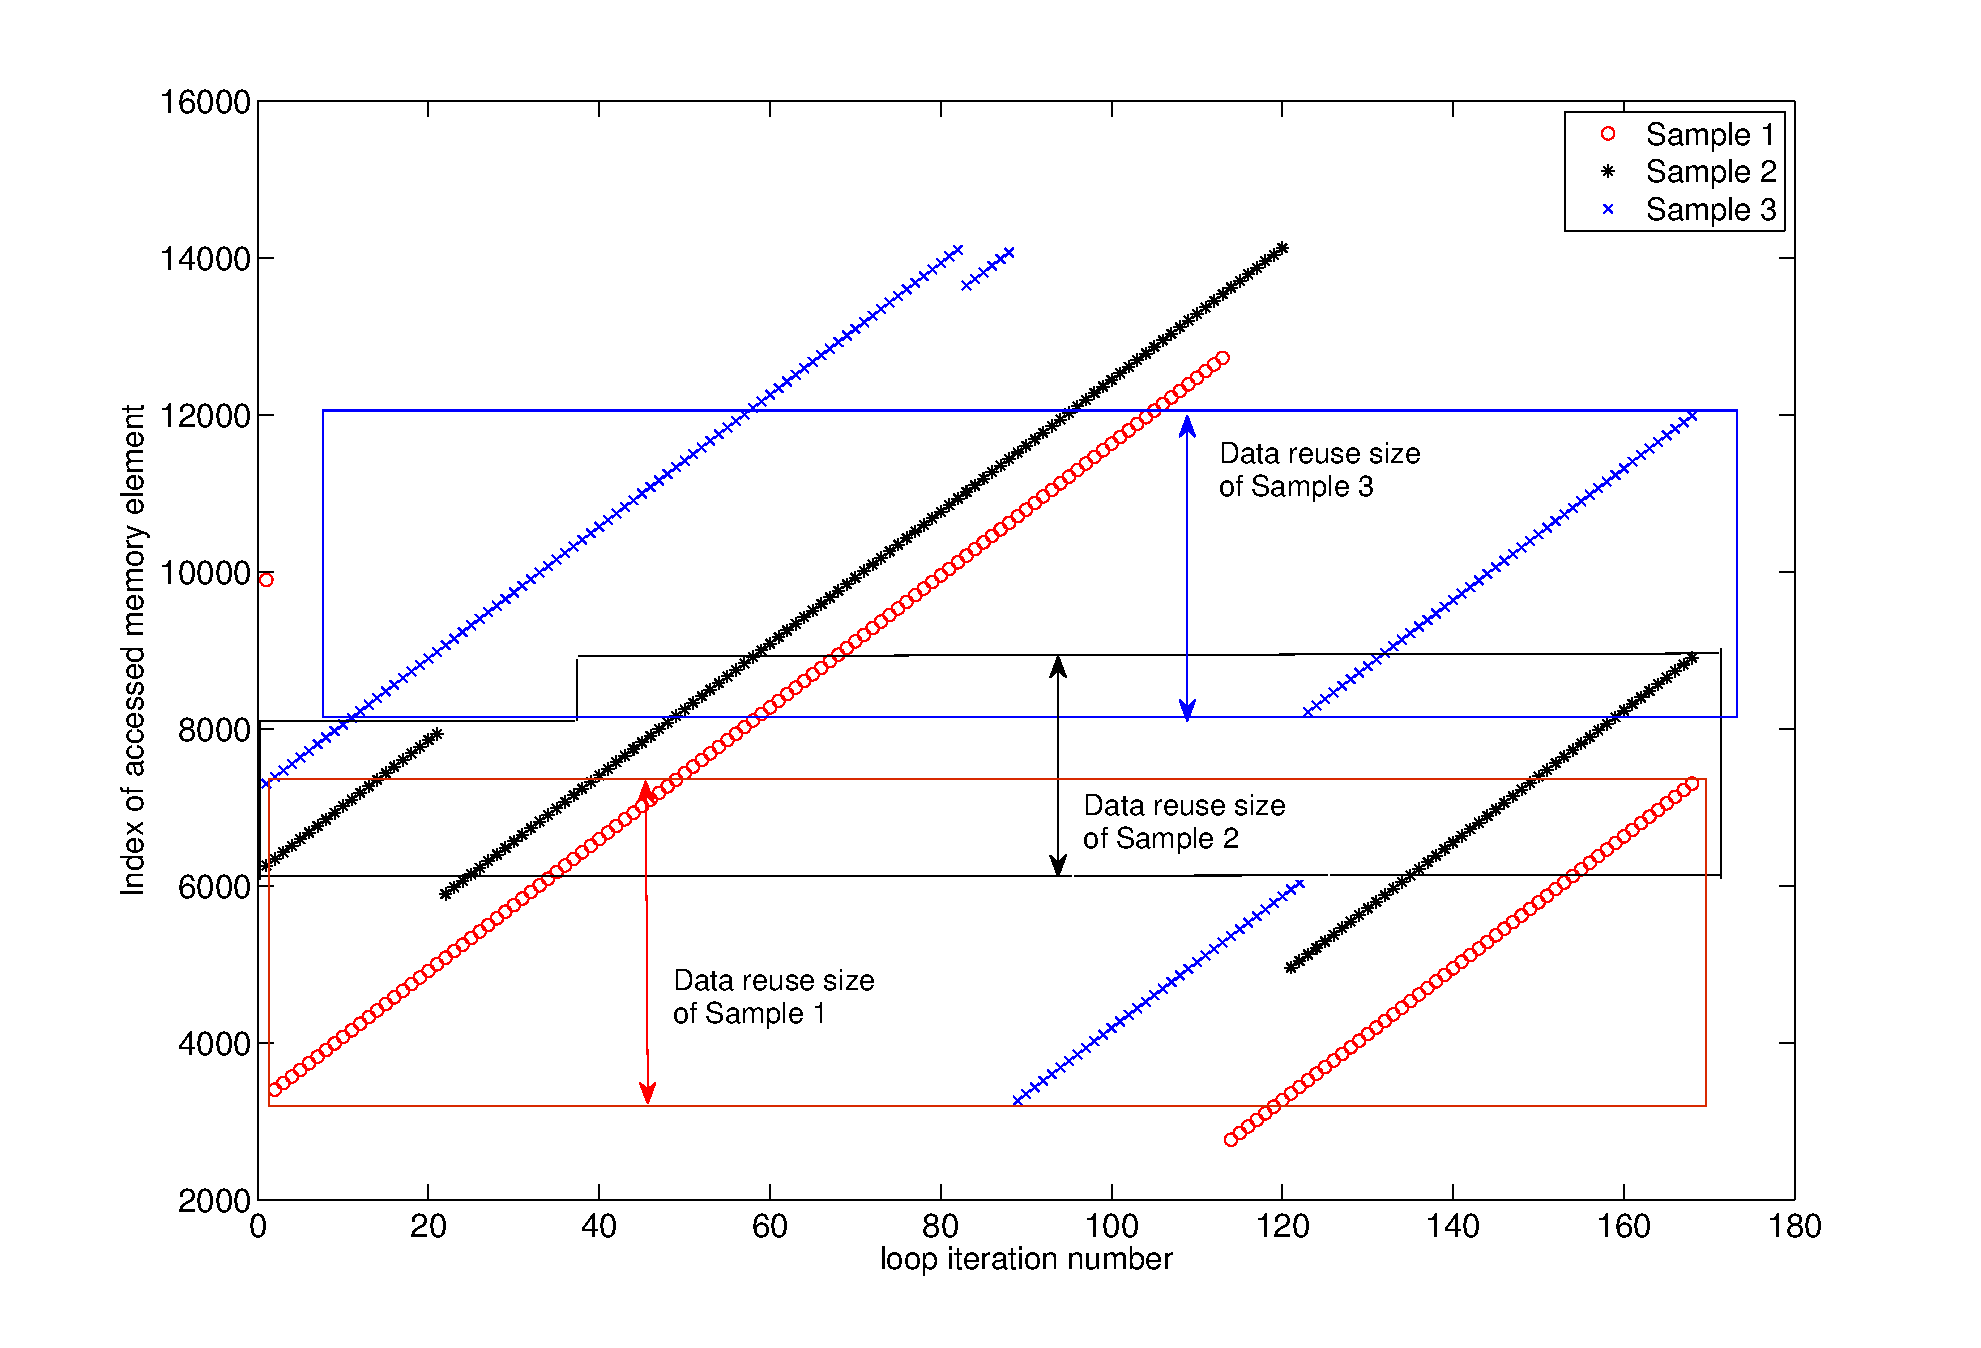
\includegraphics[width=0.8\textwidth]{A/eegprof_v1-eps-converted-to.pdf}
\caption{Memory access pattern of epilepsy predictor. Profiling of data reuse size for 3 samples from a given (\cite{Iasemidis2005}) database. The number of elements accessed is input dependent. Only those of the 16K elements accessed multiple times should be saved in L1'. The rest are accessed from L1.}
\label{fig:eegprof}
\end{figure}

Based on profiling results, scenario generation can be performed. Two possible clustering solutions are used in this paper, both of them consisting of five scenarios. In the first clustering, the range of memory indexes is split in equally sized partitions.  In the second clustering, the range is split based on occurrence frequency, so that each scenario has almost equal number of occurrences. The reconfigurable memory platform is instantiated accordingly in our target template outlined in Section \ref{sec:platform}. It contains four equal memory banks of size 975 in the first case and four banks of increasing size (195, 585, 1170, and 1950) in the second case, since smaller sizes are used more often. 

\subsection{Viterbi Algorithm Encoder}

The Viterbi algorithm \cite{viterbi} is widely used, both in the industry and academia, as an encoding/decoding algorithm for convolutional codes. As part of the encoding of the transmitted signal, redundant bits are added, which are later used by the decoder for correction of transmission errors. The output of an encoder is a function of current input bit(s) and K earlier inputs, where K is the constraint length of the algorithm. Profiling shows that the constraint length dominates the memory cost.  In Tab.~\ref{tab:snr} \cite{avd} constraint length values to achieve $ 10^{-5} $ BER are presented for different noise levels in the channel. Due to its limited range of values, the constraint length is classified as a control variable. The scenario generation is based on profiling and aims at achieving a consistent bit error rate with the minimum memory usage. If SNR \nomenclature{SNR}{signal to noise ratio} decreases, another memory bank is activated while reduction in channel noise leads to the opposite effect. The L1' sizes can be found in Tab.~\ref{tab:snr}. Clustering has been performed for K-values 5 and 6, with a resulting L1' size of 48B, and between K-values 8 and 9, with a resulting L1' size of 72B

\begin{table}[!t]
\caption{Constraint length for SNR levels on the channel (BER $ \leqslant 10^{-5} $)}
\label{tab:snr}
\centering
\begin{tabular}{|c|c|c|c|c|c|}
\hline 
SNR (dB) & K & L1' size (B) & SNR (dB) & K & L1' size (B) \\ 
\hline 
6,5 - 6,1 & 5 & 40 & 3,9 - 3,1 & 9 & 72 \\ 
\hline 
6,1 - 5,5 & 6 & 48 & 3,1 - 2,8 & 12 & 96 \\ 
\hline 
5,5 - 3,9 & 8 & 64 & 2,8 - 2,5 & 14 & 112 \\ 
\hline 
\end{tabular}      
\end{table}
 
\section{Results}
\label{sec:results}

The memory aware system scenario methodology is applied to both of our benchmark applications to study its effectiveness. Memory energy consumption is calculated based on \cite{Artes2011} and is the sum of (energy per access) $ \times $ (number of accesses) and energy costs for all transitions between memory modes. The energy for each access is defined by the type and the size of the accessed memory. Based on profiling and scenario generation results, four different memory organizations are compared for the epileptic seizure predictor. The first one is a scenario strategy without memory awareness and use a single memory bank large enough to satisfy the most demanding sample. That approach is the worst case for the memory size and statically allocates the highest value of the memory space demanded during the lifetime of the application, i.e., 3900. However, the number of accesses to the memory will be determined by each sample and no worst case assumption is made for number of accesses.

The second approach assumes that L1' has four banks of the same size (975) that can be turned on and off. The third one assumes an L1' with four banks with different sizes (195, 585, 1170, and 1950), in order to better exploit RTSs with small memory footprints.  Finally, a theoretical lower bound assumes an unlimited number of memory banks in all sizes to optimally exploit every situation. Comparison results are shown in Fig.~\ref{fig:gainsEEG} and memory energy gains up to 40\% are achieved with the scenario methodology for dynamic input samples. The high quality of our results is substantiated by the fact that our energy consumption is very close to the theoretical lower bound, even though the latter is impossible due to limited area in embedded devices.  

\begin{figure}[!t]
\centering
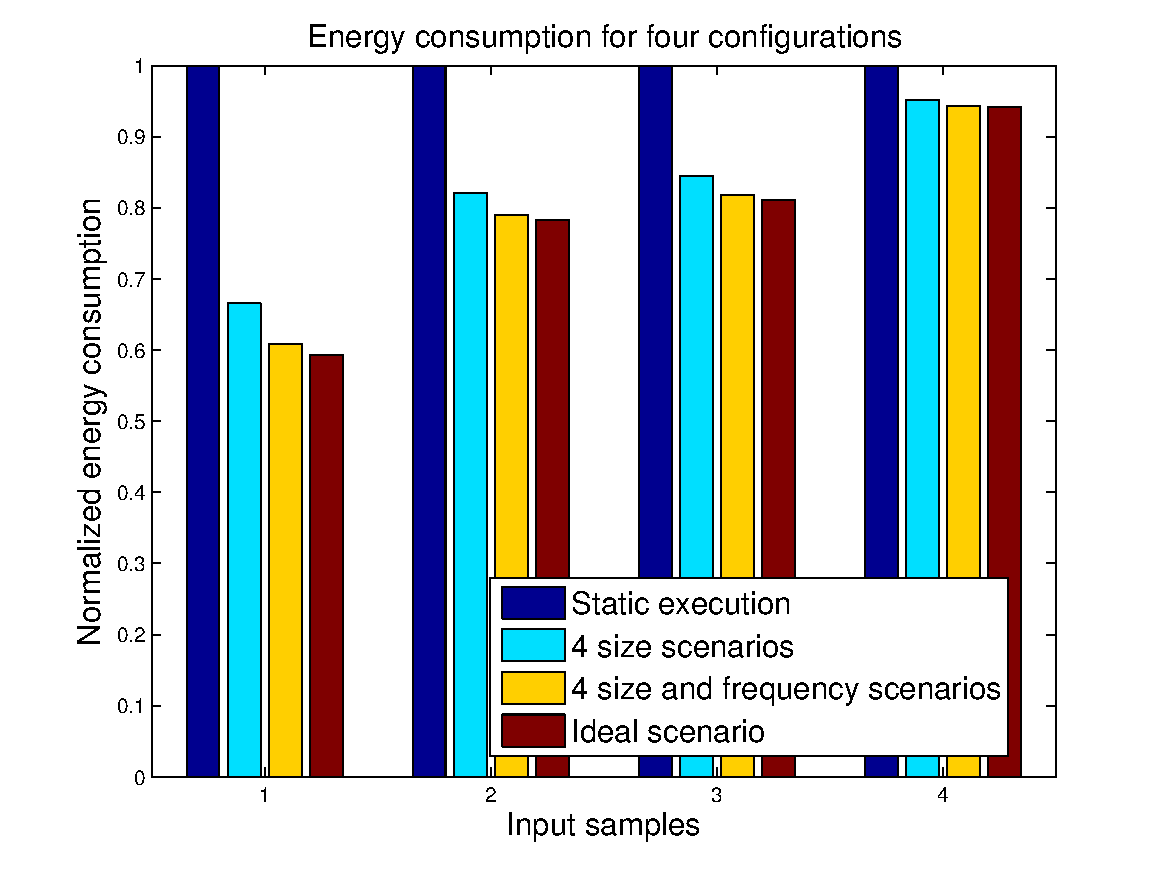
\includegraphics[width=\textwidth]{A/results1-eps-converted-to.pdf}
\caption{Memory-aware scenario gains - Epileptic seizure predictor}
\label{fig:gainsEEG}
\end{figure}

\begin{figure}[!t]
\centering
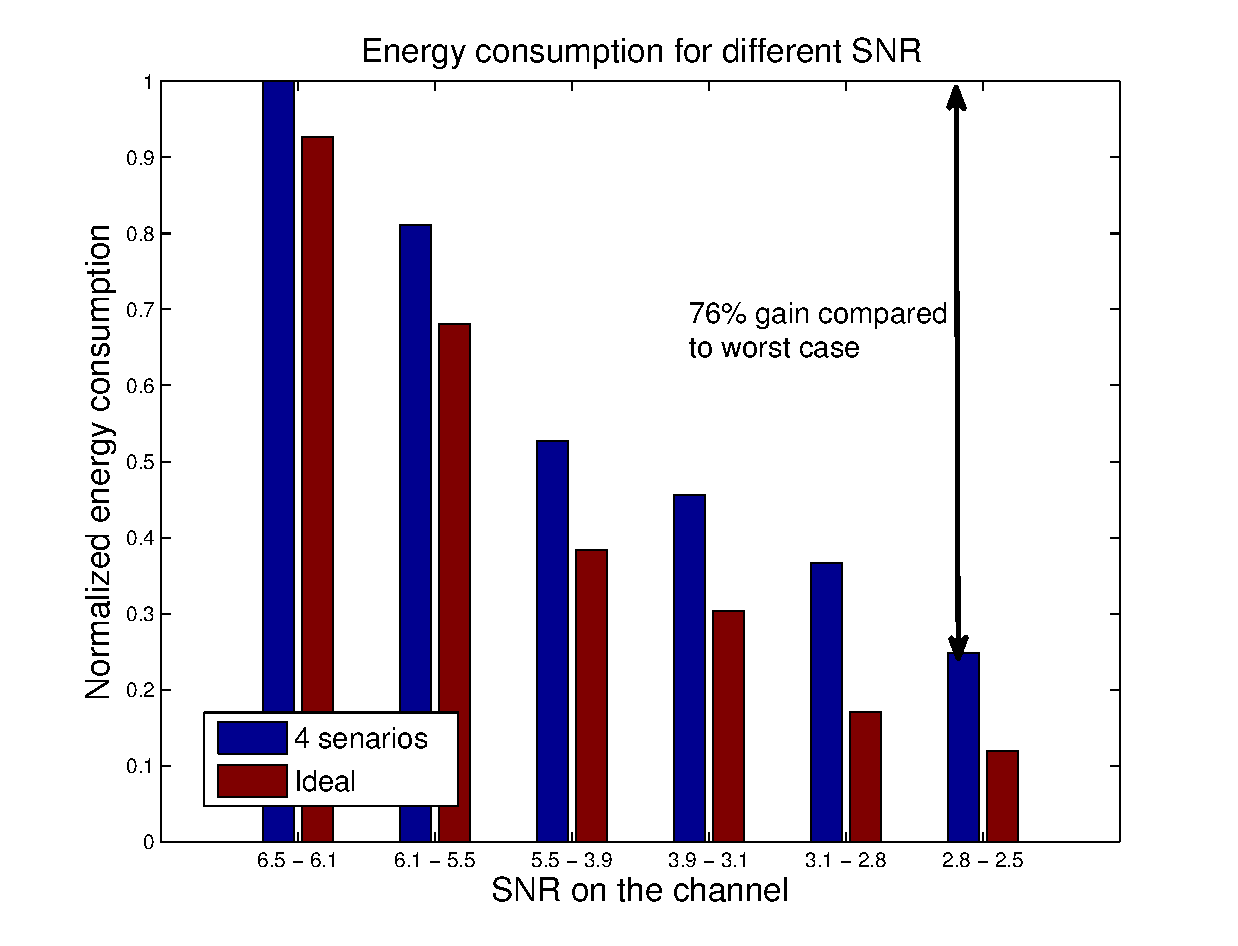
\includegraphics[width=\textwidth]{A/res2-eps-converted-to.pdf}
\caption{Memory-aware scenario gains - Viterbi encoder}
\label{fig:gainsViterbi}
\end{figure}

Even higher gains are found for the Viterbi encoder (Fig.~\ref{fig:gainsViterbi}) compared to a worst-case assumption of the constraint length being equal to 14. That value of length is used to achieve acceptable BER \nomenclature{BER}{bit error rate} over very noisy channels. Using the extended system scenario methodology, L1' is split into four smaller banks that can be turned off when the noise of the channel is reduced. Again, the theoretical lower bound assumes a memory organisation with bank sizes optimized for each SNR level. Its hardware implementation would need 24 memory banks instead of 4 in our case, which leads to an unacceptable overhead. The proposed reconfigurable memory organisation can lead to more than 70\% reduction in memory energy consumption in situations with low noise, compared to a static architecture that is tuned to handle SNR levels down to 2.5 dB.

\section{Conclusion}
\label{sec:conclusion}

The scope of this work is to extend the existing system scenario techniques to better take memory into account. The memory-aware system scenario methodology has been described and tested on two real applications from bioengineering and wireless communications domains. Results justify the effectiveness of the methodology in reduction of memory energy consumption, which is of great importance in embedded devices. Since memory size requirements are still met in all situations, performance is not reduced. The memory-aware system scenario methodology is suited for applications that experience dynamic behaviour with respect to memory organisation utilization during their execution.

\addcontentsline{toc}{section}{Bibliography}	
\bibliographystyle{plain}
\bibliography{reference}
 
%\chapter{Exploration of energy efficient memory organisations for dynamic multimedia applications using system scenarios}

\begin{center}
Iason Filippopoulos, Francky Catthoor and Per Gunnar Kjeldsberg
\\
Memory Architecture and Organization Workshop
\\
Embedded Systems Week
\\
2013
\end{center}
\afterpage{\null\newpage}
\newpage

\vspace*{\fill}
%\addcontentsline{toc}{section}{Abstract}
\section*{\hspace*{\fill} Abstract \hspace*{\fill}}
We propose a memory-aware system scenario approach that exploits variations in memory needs during the lifetime of an application in order to optimize energy usage. Different system scenarios capture the application's different resource requirements which change dynamically at run-time. In addition to computational resources, the many possible memory platform configurations and data-to-memory assignments are important system scenario parameters. Here we present an extended memory model that includes existing state-of-the-art memories, available in the industry and academia, and show how it is employed during the system design exploration phase. Both commercial SRAM and standard cell based memory models are explored in this study. The effectiveness of the proposed methodology is demonstrated and tested using a large set of multimedia benchmarks published in the Polybench, Mibench and Mediabench suites. Reduction in energy consumption in the memory subsystem ranges from 35\% to 55 \% for the chosen set of benchmarks.
\vspace*{\fill}
\afterpage{\null\newpage}
\newpage

\section{Introduction}
%\label{sec:introduction}

Modern embedded systems are becoming more and more powerful as the semiconductor processing techniques keep increasing the number of transistors on a single chip. Consequentially, demanding applications, e.g., in the signal processing and multimedia domains, can be executed on these devices \cite{narasinga}. On the other hand, the desired performance has to be delivered with minimum power consumption due to the limited energy available in mobile devices \cite{tcm}. System scenario methodologies propose the use of different platform configurations in order to exploit run-time variations in computational and memory needs often seen in such applications \cite{tcm}.

%Francky: explain about the knobs
Platform reconfiguration is performed through tuning of different system parameters, also called system knobs. For the memory-aware system scenario methodology, a platform can be reconfigured through a number of potential knobs, each resulting in different performance and power consumption in the memory subsystem. Foremost, modern memories support different energy states, e.g., through power gating techniques and by switching to lower power modes when not accessed. %removed for blind \cite{Fil12}
The second platform knob is the assignment of data to the available memory banks. The data assignment decisions affect both the energy per access for the mapped data, the data conflicts as a result of suboptimal assignment, and the number of active banks. In this work a reconfigurable memory platform is constructed using detailed memory models. This is followed by experiments with dynamic multimedia applications in order to study the effectiveness of the methodology.

%Domain specific for ESTIMedia + comparison with use case
%in comparison with \cite{Fil12} 
%, which is potentially applicable to every multimedia application with dynamic memory usage. 
The main contribution of the current work is the development of data variable based system scenarios. Previous control variable based system scenarios are unable to handle the fine-grain behaviour of the studied multimedia applications due to their significant variation under different execution situations. Furthermore, compared with use case scenario approaches in which scenarios are generated based on a user's behaviour, the system scenario methodology focuses on the behaviour of the system to generate scenarios and can, therefore, fully exploit the detailed platform mapping information. Rather than focusing on the processing cores, this work analyses the application of system scenarios on the memory organisation. Other contributions are for the purpose sufficiently detailed and accurate memory models used for the system design exploration, an extensive number of benchmark applications on which the methodology is applied, and a categorisation of applications based on their dynamic characteristics. For the multimedia domain, the current work presents a comprehensive methodology for optimising energy consumption in the memory subsystem.

%It still means we can have measurable differences,
%in particular that we are exploiting data variable system scenarios (that - the data variables
%exploit detailed platform mapping information) instead
%of control variable sys-scen (which cannot handle our applications due
%to too fine grain scenario behaviour in the data variables) or use case scen
%(which do not exploit any detailed platform mapping info).
%And compared to the limited work that targets data variable sys-scen, we
%now focus on memory organ instead of the processor cores.
%I assume you can formulate a few sentences around the above?
%Most of the dynamic variables in the current work can be classified as data variables due to their significant variation under different execution situations. 

%This paper is organized as follows. Section~\ref{sec:motivation} motivates the study of optimization of the memory organisation and surveys related work on system level memory exploration. Section~\ref{sec:methodology} presents the chosen methodology with main focus on the memory organisation study. In Section~\ref{sec:platform} the target platform is described accompanied by a detailed description of the employed memory models, while the multimedia benchmarks and their characteristics are analysed in Section~\ref{sec:applications}. Results of applying the described methodology to the targeted applications are shown in Section~\ref{sec:results}, while conclusions are drawn in Section~\ref{sec:conclusion}. 

\section{Motivation and Related Work}
%\label{sec:motivation}

A large number of papers have demonstrated the importance of the memory organization to the overall system energy consumption. Especially for embedded systems, the memory subsystem accounts for up to 50\% of the overall energy consumption \cite{Che09} and the cycle-accurate simulator presented in \cite{Ben99} estimates that the energy expenditures in the memory subsystem range from 35\% up to 65\% for different architectures. According to \cite{tcm}, conventional allocation and assignment of data done by regular compilers is suboptimal. Performance loss is caused by stalls for fetching data and data conflicts for different tasks, due to the limited size of memory and the competition between tasks.The significant contribution that the memory subsystem has to the overall energy consumption of a system and the dynamic nature of many applications offer a strong motivation for the study and optimization of the memory organisation in modern embedded devices.

Many papers have focused on memory related optimisations, also in the presence of a partitioned and distributed memory organisation with memory blocks of different sizes. In \cite{Ben00b} authors present a methodology for automatic memory hierarchy generation that exploits memory access locality, while in \cite{Ben00c} they propose an algorithm for the automatic partitioning of on-chip SRAM in multiple banks. Several design techniques for designing energy efficient memory architectures for embedded systems are presented in \cite{Mac02}. The current work differentiates by employing a platform that is reconfigurable during run-time. In \cite{Pgk01} a large number of data and memory optimisation techniques, that could be dependent or independent of a target platform, are discussed. Again, reconfigurable platforms are not considered.

Energy-aware assignment of data to memory banks for several task-sets based on the MediaBench suit of benchmarks is presented in \cite{Mar03}. Low energy multimedia applications are discussed also in \cite{Chu02} with focus on processing rather than the memory platform. Furthermore, both \cite{Mar03} and \cite{Chu02} base their analysis on use case situations and do not incorporate sufficient support for very dynamically behaving application codes. System scenarios alleviate this bottleneck and enable handling of such dynamic behaviour. In addition, the current work explores the assignment of data to the memory and the effect of different assignment decisions on the overall energy consumption.

%An overview of work on system scenario methodologies and their application are presented in \cite{Gheorghita2007}. In \cite{Fil12} extensions towards a memory-aware system scenario methodology are presented and demonstrated using theoretical memory models and two target applications. This work is an extension both in complexity and accuracy of the considered memory library and on the number of target applications. 

\section{Data Variable Based Memory-Aware System Scenario Methodology}
%\label{sec:methodology}
%PKG: Remove most of the citations to Norchip

%The memory-aware system scenario methodology is based on the observation that the memory subsystem requirements at run-time vary significantly due to dynamic variations of memory needs in the application code. Most existing design methodologies define the memory requirements as that of the most demanding task and tune the system in order to meet its needs \cite{tcm}. Obviously, this approach leads to unused memory area for tasks with lower memory requirements, since those tasks could meet their needs using fewer resources and consequentially consuming less energy. Another source of unnecessary waste of energy in the memory is caused by data conflicts due to misplaced data. Replacement of old data and fetching of new data is both time and energy consuming and should therefore be avoided. Handling of data conflicts is also part of a memory-aware system scenario methodology.

Designing with system scenarios is workload adaptive and offers different configurations of the platform and the freedom of switching to the most efficient scenario at run-time. A system scenario is a configuration of the system that combines similar run-time situations (RTSs). An RTS consists of a running instance of a task and its corresponding cost (e.g., energy consumption) and one complete run of the application on the target platform represents a sequence of RTSs \cite{Elena2010}. The system is configured to meet the cost requirements of an RTS by choosing the appropriate system scenario, which is the one that satisfies the requirements using minimal power. In the following subsections, the different steps of the memory-aware system scenario methodology are outlined. 

The general system scenario methodology follows a two stage exploration, namely design-time and run-time stages, as described in \cite{Gheorghita2007}. This splitting is also employed in the memory-aware extension of the methodology. The two stage exploration is chosen because it reduces run-time overhead while preserving an important degree of freedom for run-time configuration \cite{tcm}. The application is analysed at design-time and different execution paths causing variations in memory demands are identified. This procedure, which is time consuming and as a result can be performed only during the design phase, will result in a grey-box model representation of the application. The grey-box model hides all static and deterministic parts of the application, by providing only related memory costs for those, and keeps parts of the application code that are non-deterministic in terms of memory usage available to the system designer \cite{graybox}. 


\subsection{Design-time Profiling Based on Data Variables}

\begin{figure}[!t]
\centering
\includegraphics[width=\textwidth]{B/Images/profiling2.pdf}
\caption{Profiling results based on application code and input data}
\label{fig:profiling}
\end{figure}

Application profiling is performed at design-time for a wide range of inputs. The analysis focuses on the allocated memory size during execution and on access pattern variations. Techniques described in \cite{Ang13b} are, e.g., used in order to extract the access scheme through analysis of array iteration spaces.  

The profiling stage is depicted in Fig.~\ref{fig:profiling} and consists of running the application code with suitable input data often found in a database, in order to produce profiling results. The results shown here are limited for demonstrational purposes. A real application would have thousands or millions of profiling samples. The profiling reveals parts of the application code with high memory activity and with varying memory access intensity, which possibly depends on input data variables. Because of this behaviour, a static study of the application code alone is insufficient since the target applications for this methodology have non-deterministic behaviour that is driven by input.

%Given code and database with data inputs, profiling will show memory usage during run-time.
%% PGK suggests deleting: by running the application using the whole database as an input. 
%Results provided to the designer include complete information about allocated memory size values together with the number of occurrences and duration for each of these memory size values. Moreover, correlation between input data variable values and the resulting memory behaviour can possibly be observed. This information is useful for the clustering step that follows. 

In Fig.~\ref{fig:profiling} the profiled applications are two image related multimedia benchmarks and the input database should consist of a variety of images. The memory requirements in each case are driven by the current input image size, which is classified as a data variable due to the wide range of its possible values. Depending on the application the whole image or a region of interest is processed. 
Other applications have other input variables deciding the memory requirement dynamism, e.g., the SNR level on the channel in the case of an encoding/decoding application.

\subsection{Design-time System Scenario Identification and Prediction Based on Data Variables}

\begin{figure}[!t]
\centering
\includegraphics[width=\textwidth]{B/Images/1DclusteringShort.pdf}
%\includegraphics[angle=270, width=0.47\textwidth]{Images/1Dclustering.ps}
\caption{Clustering of profiling results into three (a) or five (b) system scenarios}
\label{fig:clustering}
\end{figure}

The next step is the clustering of the profiled memory sizes into groups with similar characteristics. This is referred to as system scenario identification. Clustering is necessary, because it will be extremely costly to have a different scenario for every possible size, due to the number of memories needed. Clustering neighbouring RTSs is a rational choice, because two instances with similar memory needs have similar energy consumption. In Fig.~\ref{fig:clustering} the clustering of the previously profiled information is presented. The clustering of RTSs is based both on their distance on the memory size axis and the frequency of their occurrence. Consequently, the memory size is split unevenly with more frequent RTSs having a shorter memory size range. This is better than even splitting because the energy cost of each system scenario is defined by the upper size limit, as each scenario should support all RTSs within its range. With more scenarios, e.g., five instead of 3, the aggregated RTS running overhead is reduced. Still the number of scenarios should be limited due to overhead of a complex memory platform and of frequent switching between scenarios.

The design-time system scenario prediction phase consists of determination of the data variables that define the active system scenario. This can be achieved by careful study of the application code, combined with the application's data input. In our case the grey-box model reveals only the code parts that will influence memory usage, so that data variables deciding memory space changes can be identified. An example of this is a non static variable that influences the number of iterations for a loop that performs one memory allocation at each iteration. In the depicted example the system scenario prediction data variable is the input image height and width values. Moreover, the designer should look for a correlation between input values and the corresponding cost. This information will be useful in the following steps of the methodology \cite{tcm}.


\subsection{Run-time System Scenario Detection and Switching Based on Data Variables}

Switching decisions are taken at run-time by the run-time manager. The switching phase consists of all platform configuration decisions that can be made at run-time, e.g., frequency/voltage scaling, changing the power mode of memory units, including turning them off, and reassignment of data on memory units. Switching takes place when the switching cost is lower than the energy gains achieved by switching. In more detail, the run-time manager compares the memory energy consumption of executing the next task in the current active system scenario with the energy consumption of execution with the optimal system scenario. If the difference is greater than the switching cost, then scenario switching is performed \cite{tcm}. Switching costs are defined by the platform and include all memory energy penalties for run-time reconfigurations of the platform, e.g., extra energy needed to change state of a memory unit.

\begin{figure}[!t]
\centering
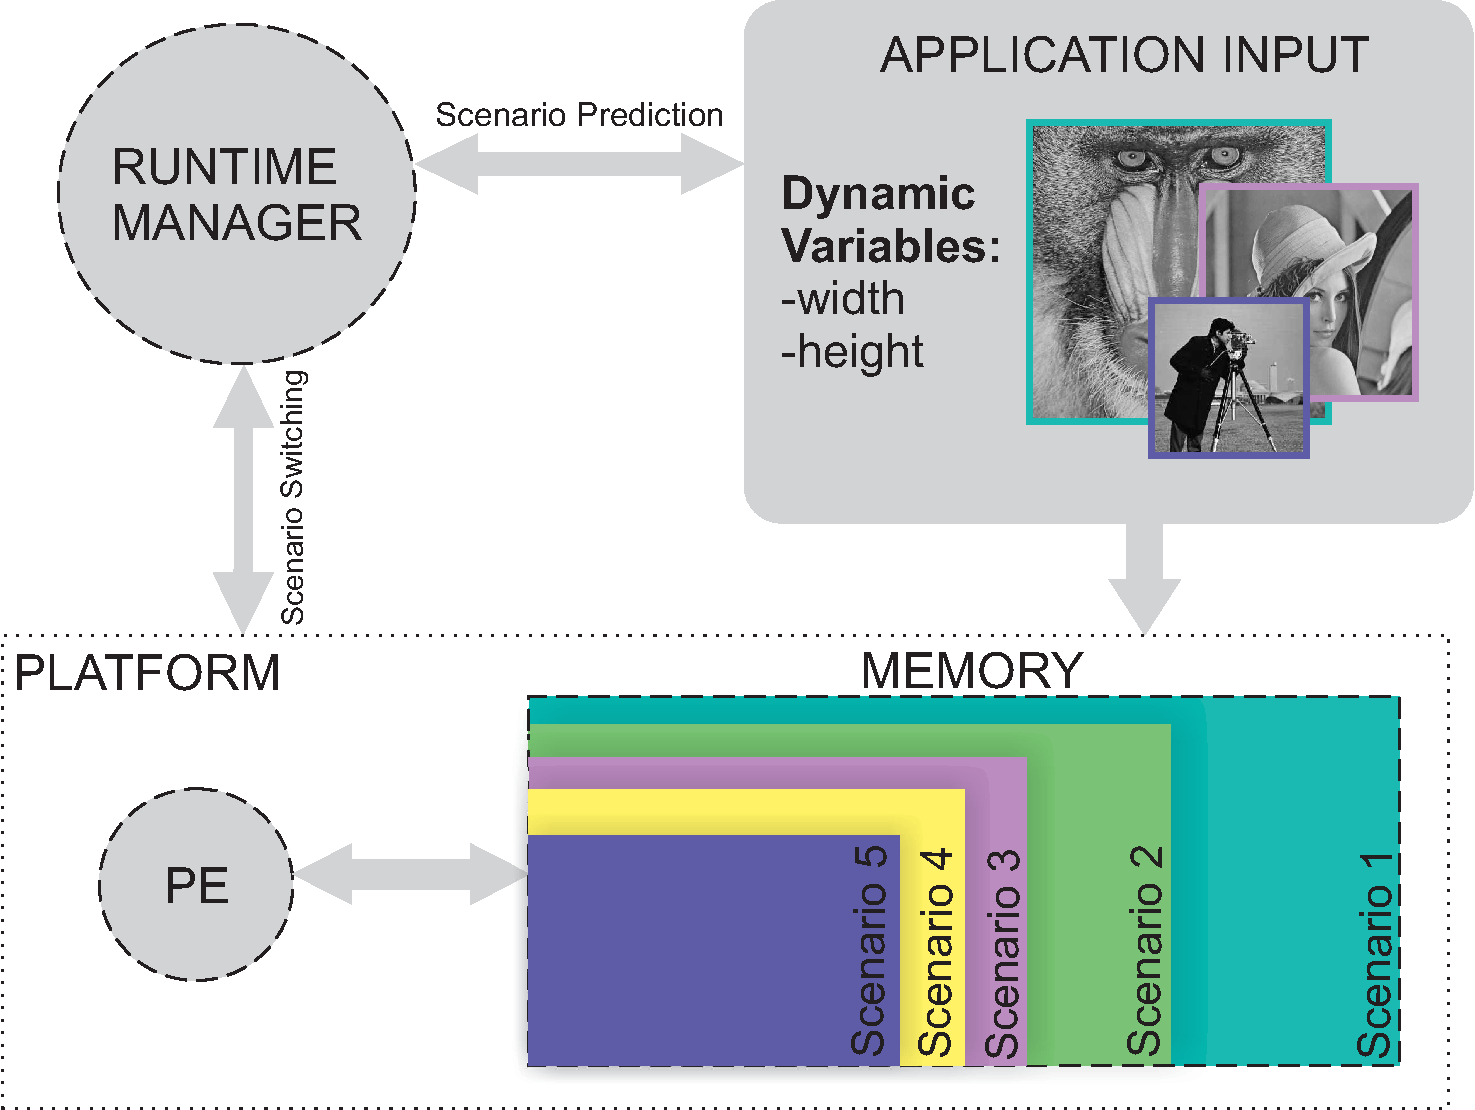
\includegraphics[width=\textwidth]{B/Images/switching.pdf}
\caption{Run-time system scenario prediction and switching based on the current input}
\label{fig:runtime}
\end{figure}

In Fig.~\ref{fig:runtime} an example of the run-time phase of the methodology is depicted. The run-time manager identifies the size of the image that will be processed and reconfigures the memory subsystem on the platform, if needed, by increasing or decreasing the available memory size. The reconfiguration options are effected by platform hardware limitations. The image size is the data variable monitored in order to detect the system scenario and the need for switching.

\section{Target Platform and energy models}
%\label{sec:platform}

Selection of target platform is an important aspect of the memory-aware system scenario methodology. The key feature needed in the platform architecture is the ability to efficiently support different memory sizes that correspond to the system scenarios generated by the methodology. The dynamic memory platform is achieved by organising the memory area in a varying number of banks that can be switched between different energy states. In this work, a clustered memory organisation with up to five memory banks of varying sizes is explored. Some examples of alternative memory platforms that can be used for exploration is shown in Fig.~\ref{fig:platform}.

\begin{figure}[!t]
\centering
\includegraphics[width=\textwidth]{B/Images/platform.pdf}
\caption{Alternative memory platforms with varying number of banks}
\label{fig:platform}
\end{figure}

%For more complex architectures the interconnection cost should be considered and analysed separately for accurate results. Although power gating can be applied to the bus when only a part of a longer bus is needed, an accurate model of the memory wrapper and interconnection must developed, which is beyond the scope of the current work.  Point-to-point connections with negligible interconnect costs between elements are assumed for up to five memory banks.

\subsection{Models of Different Memory Types}

The dynamic memory organisation is constructed using commercially available SRAM memory models (MM). In addition, experimental standard cell-based memories (SCMEM) \cite{Mei11}  are  considered for smaller memories due to their energy and area efficiency for reasonably small storage capacities, as argued in \cite{Mei10}. Both MMs and SCMEMs can operate under a wide range of supply voltages, thus support different operating modes that provide an important exploration space. In the active mode the memory can be accessed at the maximum supported speed and the supply voltage is set at 1.1V. While data are not accessed for a period of time the light/deep sleep or shut down mode should be considered. In light sleep mode the supply voltage is lowered with values around 0.7V, while on deep sleep mode the supply voltage is set to the lowest possible value that can be used without loss of data. This voltage threshold is expected to be lower for SCMEMs than MM models and can be as low as 0.3V. The shut down mode uses power-gating techniques to achieve near zero leakage power, but stored data is lost. The time and the energy required for switching from these low leakage modes to the active state differs and all the necessary energy/power information is available to the system designer.

\subsection{Energy consumption calculation}
The overall energy consumption for each configuration is calculated using a detailed formula, as can be seen in (\ref{eq:energy}). 
%\setlength{\arraycolsep}{0.0em}
%\begin{eqnarray}
%\label{eq:energy}
% E &{}= {}&\sum\limits_{memories}^{all}  ( N_{rd} \times E_{Read} \nonumber\\
%		&&+ N_{wr} \times E_{Write} \nonumber\\
%		&&+ (T-T_{LSleep}-T_{DSleep}-T_{ShutDown})\times P_{leak_{Active}} \nonumber\\
%		&&+ T_{LSleep} \times P_{leak_{LSleep}} \nonumber\\
%		&&+ T_{DSleep} \times P_{leak_{DSleep}} \nonumber\\
%		&&+ T_{ShutDown} \times P_{leak_{ShutDown}} \nonumber\\ 
%		&& + N_{SWLight} \times E_{LSleep \: to \: Active} \nonumber\\
%		&& + N_{SWDeep} \times E_{DSleep \: to \: Active} \nonumber\\
%		&& + N_{SWShutDown} \times E_{ShutDown \: to \: Active} ) \nonumber\\
%\end{eqnarray}
%\setlength{\arraycolsep}{5pt}
\begin{equation}
\label{eq:energy}
\begin{array}{lcl}
E&=&\sum\limits_{memories}^{all}  ( N_{rd} \times E_{Read}+ N_{wr} \times E_{Write}\\
&+&(T-T_{LSleep}-T_{DSleep}-T_{ShutDown})\times P_{leak_{Active}}\\
&+&T_{LSleep} \times P_{leak_{LSleep}}+T_{DSleep} \times P_{leak_{DSleep}}\\
&+&T_{ShutDown} \times P_{leak_{ShutDown}}\\
&+&N_{SWLight} \times E_{LSleep \: to \: Active}\\
&+&N_{SWDeep} \times E_{DSleep \: to \: Active}\\
&+&N_{SWShutDown} \times E_{ShutDown \: to \: Active} )\\
\end{array}
\end{equation}
					
All the important transactions on the platform that contribute to the overall energy are included, in order to achieve as accurate results as possible. In particular:
\begin{itemize}
\item $N_{rd}$ is the number of read accesses
\item $E_{Read}$ is the energy per read
\item $N_{wr}$ is the number of write accesses 
\item $E_{Write}$ is the energy per write 
\item T is the execution time of the application
\item $T_{LSleep}$, $T_{DSleep}$ and $T_{ShutDown}$ are the times spent in light sleep, deep sleep and shut down states respectively
\item $P_{leak_{Active}}$ is the leakage power in active mode 
\item $P_{leak_{LSleep}}$, $P_{leak_{DSleep}}$ and $P_{leak_{Shutdown}}$ are the leakage power values in light sleep, deep sleep and shut down modes with different values corresponding to each mode 
\item $N_{SWLight}$, $N_{SWDeep}$ and $N_{SWShutDown}$ are the number of transitions from each retention state to active state
\item $E_{LSleep \: to \: Active}$, $E_{DSleep \: to \: Active}$ and \\ $E_{ShutDown \: to \: Active}$  are the energy penalties for each transition respectively.
\end{itemize}

 The overall energy consumption is given after calculating the energy for each memory bank. The execution time of the application is needed to calculate the leak time. It can be found by executing the application on a reference embedded processor. The simulator described in \cite{Gem5} is chosen to calculate execution time for the chosen applications in this work. The processor is assumed to be running continuously, accepting new input data as soon as computations on the previous data set has been finished. Memory sleep times are hence only caused by data dependent dynamic behaviour.

\subsection{Architecture Exploration}

The exploration of alternative memory platforms is performed using the steps described in Alg.~\ref{alg:clustering}. All potentially energy efficient configurations are tested for a given number of scenarios and the sequence of RTSs of the application. First, all possible configurations for a given number of memory banks are constructed. The only requirement in order to keep a configuration for further investigation is that the combined size of all banks should satisfy the storage requirements of the most demanding RTS. Then, each configuration is tested for the sequence of RTSs and the one that minimizes Eq.\ref{eq:energy} is chosen as the most energy efficient for this number of scenarios (i.e., number of banks). 

\begin{algorithm}[!t]
\caption{Memory organisation exploration steps}
 \label{alg:clustering}
 \begin{algorithmic}[1]
		\STATE $RTSset \gets$ storage requirement for each RTS
		\STATE $Database \gets $ memory database
		\STATE $N \gets $ number of scenarios (up to 5 in this work)
			\FOR{$i = 1 \to N$}
				\FOR{all combinations of i banks in database}
				%\STATE $Platform \gets $ i banks from Database
				\IF{$\sum_{1}^{i} size(bank) \geq  size(max(RTS))$} \STATE{Keep configuration} \ENDIF
				\STATE Select configuration that minimizes Eq.\ref{eq:energy} for $RTSset$			
				\ENDFOR			
			\ENDFOR
 \end{algorithmic}
\end{algorithm}

 
\section{Application Benchmarks}
\label{sec:applicationsB}

The applications that benefit most from the memory-aware system scenario methodology are characterised by having dynamic utilization of the memory organisation during their execution. Multimedia applications often exhibit such dynamicity and are consequentially suitable candidates for the presented methodology. The effectiveness is demonstrated and tested using a variety of open multimedia benchmarks, which can be found in the Polybench \cite{Poly}, Mibench \cite{mibench} and Mediabench \cite{mediabench} benchmark suites. 

An overview of the benchmark applications that were tested is presented in Tab.~\ref{tab:applications}. Two key parameters under consideration are the dynamic data variable of each application and the variation in the memory requirement it causes. The dynamic data variable is the variable that results in different system scenarios due to its range of values. Examples of such a variable are an input image of varying size or data dependent loop bound values. For each application an appropriate input database is constructed with realistic RTS cases. The memory size limits are defined as the minimum and maximum storage requirement occurred during testing of an application. The dynamic characteristics that are used to categorize the applications are the dynamism in the memory size bounds and the variance of cases within the memory size limits.

The memory size bounds correspond to the minimum and maximum memory size values profiled over all possible cases. In general, larger distances between upper and lower bounds increase the possibilities for energy gains. This is a result of using larger and more energy hungry memories in order to support the memory requirements for the worst case even when only small memories are required. Large energy gain is expected when large parts of the memory subsystem can be switched into retention for a long time. 

\begin{landscape}
\clearpage
\thispagestyle{empty}
%\begin{center}
%\vspace*{\fill}
\begin{table}
\centering
\caption{Benchmark applications overview}
\label{tab:applications}
{\small
\hfill{}
\begin{tabular}{|c|c|c|c|c|c|}
\hline
\multirow{2}{*}{\textbf{Application}} & \multirow{2}{*}{\textbf{Source}} & \multirow{2}{*}{\parbox{4.2cm}{\textbf{Data variables used for scenario prediction}}} & \multicolumn{3}{c|}{\textbf{Dynamic Characteristics}} \\ \cline{4-6}
 & & & Memory Variation(B) & Number of cases & Distribution of cases\\ 
\hline 
Epic image compression & MediaBench & Image size & 4257 - 34609 & Average & good \\ 
\hline 
Motion Estimation & MediaBench 	& Image size & 4800 - 52800 & High & average \\ 
\hline 
Blowfish decoder & MiBench & Input file size & 256 - 5120 & Low  & poor \\ 
\hline 
Jacobi 1D Decomposition & Polybench & Number of steps & 502 - 32002 & Low  & good \\ 
\hline 
Mesa 3D & MediaBench & Loop bound & 5 - 50000 & High  & average\\ 
\hline 
JPEG DCT & MediaBench & Block size & 10239 - 61439 & High & average \\ 
\hline 
PGP encryption & MediaBench & Encryption length & 3073 - 49153 & High  & average \\ 
\hline 
Viterbi encoder & Open & Constraint length & 5121 - 14337 & Low & good \\ 
\hline 
\end{tabular}}
\end{table}
\end{landscape}

Another metric used for identification of different kinds of dynamism is the memory requirement variation. The variation takes into consideration both the number of different cases that are present within the memory requirement limits and the distribution of those cases between minimum and maximum memory size. Applications with a limited number of different cases are expected to have most of its possible gain obtained with a few platform supported system scenarios and much smaller energy gains from additional system scenarios. After this point most of the cases are already fitting one of the platform configurations and adding new configurations have a minimal impact. The opposite is seen for applications that feature a wide range of well distributed cases.

\section{Results}
%\label{sec:results}

The memory aware system scenario methodology is applied to all the presented benchmark applications to study its effectiveness. The profiling phase is based on different input for the data variables shown in Tab.~\ref{tab:applications} and is followed by the clustering phase. The execution and sleep times needed in Eq.\ref{eq:energy} are found through the profiling but are also reflected by the dynamic characteristics in Tab.~\ref{tab:applications}. Data variables are the variables used by the run-time manager in order to predict the next active scenario. The clustering is performed with one to five system scenarios. All potentially energy efficient configurations are tested for a given number of scenarios using the steps described in Alg.~\ref{alg:clustering}. For example, in the case of 2 scenarios all possible memory platforms with 2 memory banks that fulfil the memory size requirement of the worst case are generated and tested. The same procedure is performed for 3, 4 and 5 scenarios. The exploration includes memories of different sizes, technologies and varying word lengths. The energy gain percentages are presented in Fig.~\ref{fig:gains}. Energy gains are compared to the case of a fixed non-re-configurable platform, i.e., a static platform configuration with only 1 scenario. This corresponds to zero percentage gain in Fig.~\ref{fig:gains}. 

\begin{figure}[!t]
\centering
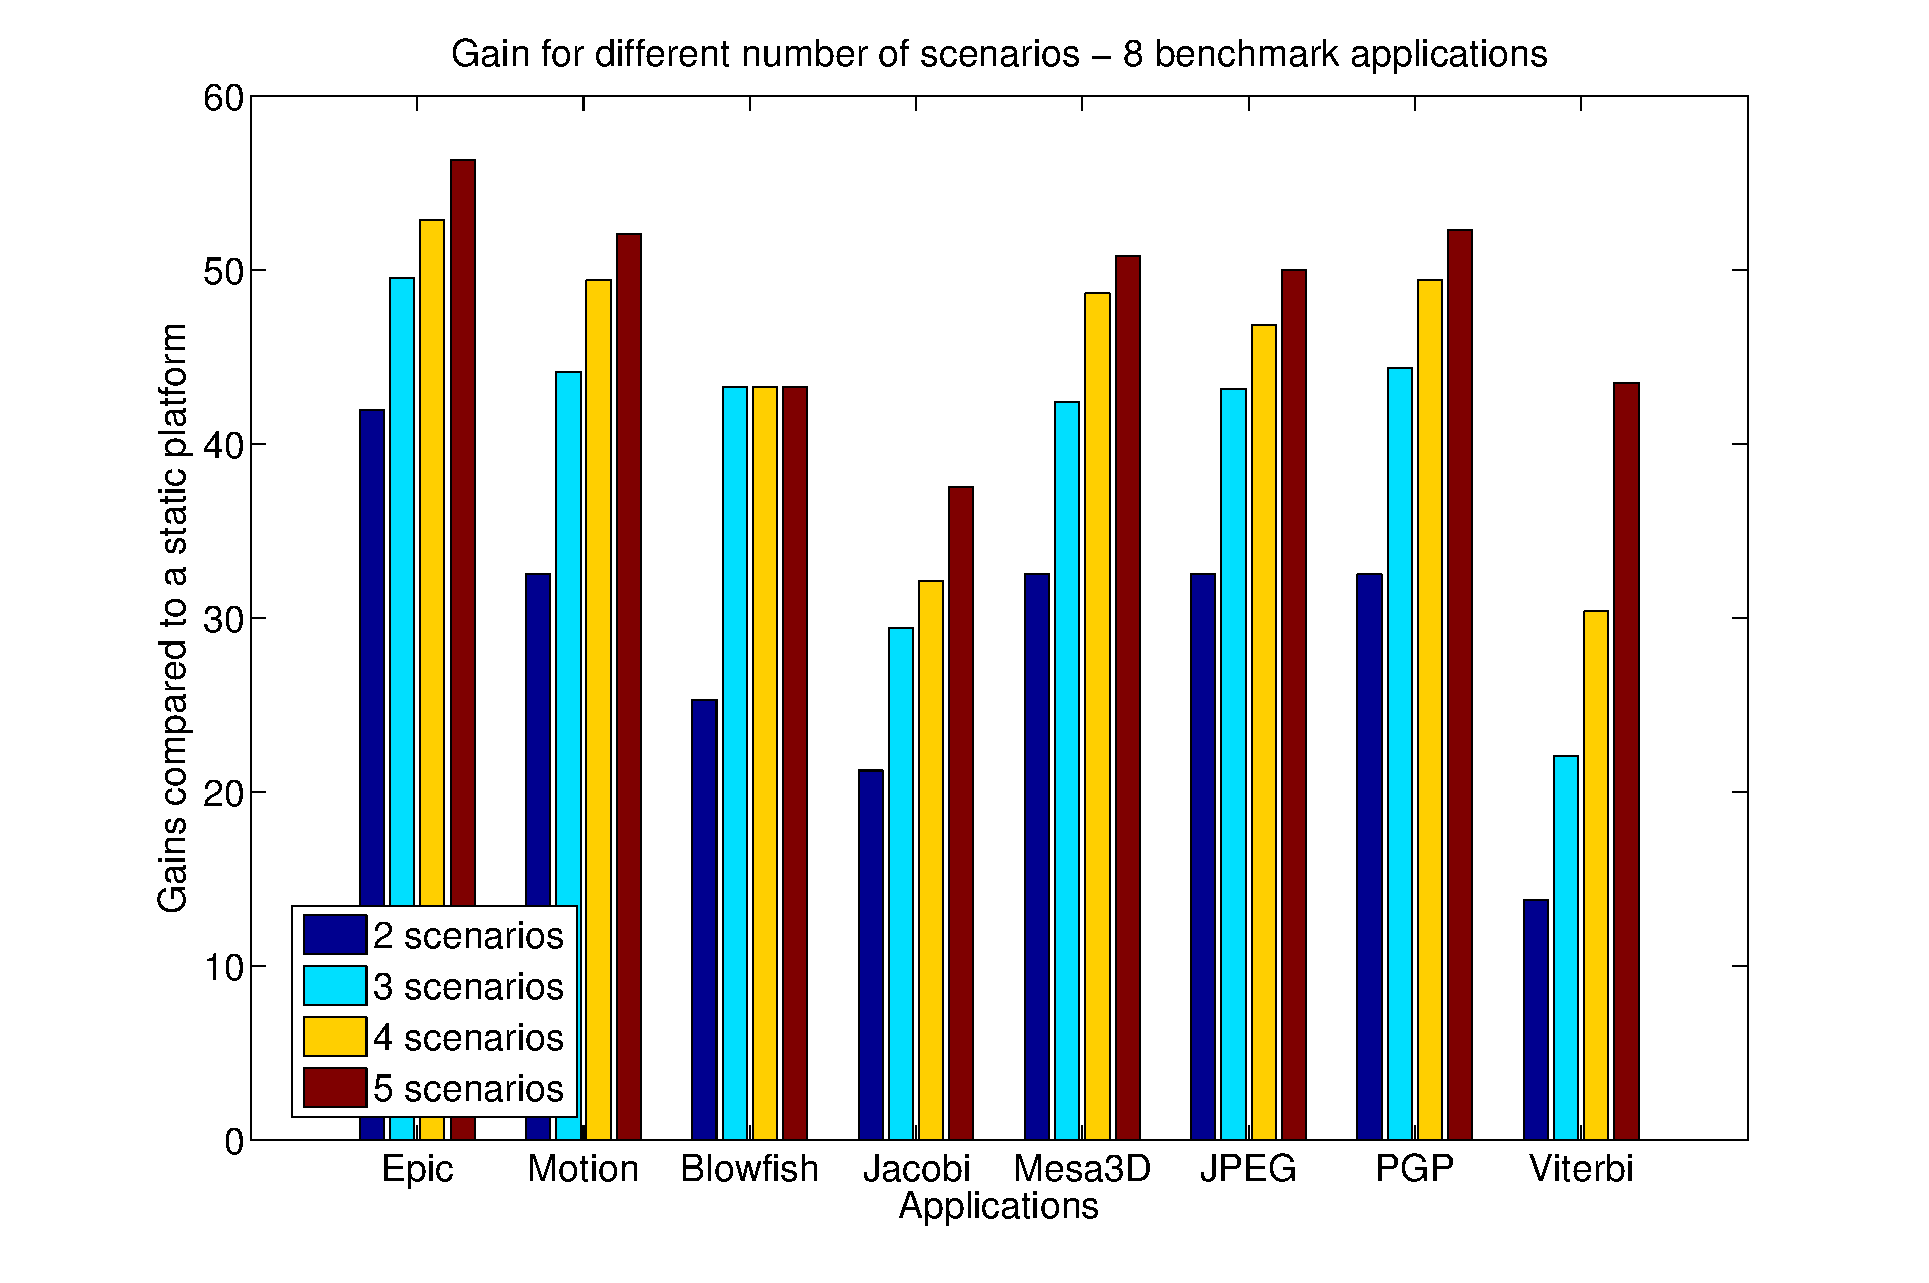
\includegraphics[width=\textwidth]{B/Images/6appsGains.pdf}
\caption{Energy gain for increasing number of system scenarios - Static platform corresponds to 0\%}
\label{fig:gains}
\end{figure}

The introduction of a second system scenario results in energy gains between 15\% and  40\%  for the tested applications. Depending on the application's dynamism the maximum reported energy gains range from around 35\% to 55\%. As expected according to the categorisation presented in subsection~\ref{sec:applicationsB}, higher energy gains are achieved for applications with more dynamic memory requirements, i.e., bigger difference between the minimum and maximum allocated size. The maximum gains for JPEG, motion estimator, mesa 3D and PGP are around 50\% while blowfish, jacobi, and Viterbi decoders are around 40\%. 

As the number of system scenarios that are implemented on the memory subsystem increases, the energy gains improve since variations in memory requirements can be better exploited with more configurations. The switching cost also increases for an increasing number of system scenarios due to the increasing frequency of platform reconfiguration. This overhead reduces the achieved gain, but for up to 5 scenarios we still see improvements for all but one of our benchmarks. The switching cost is below 2\% even for a platform with 5 memory banks in all cases. The most efficient of the tested organisations for each benchmark are presented in Fig.~\ref{fig:banks}, where each memory bank is depicted with a different colour and each length is proportional to the memory bank size. The blowfish decoder is the only benchmark that has only 3 banks in its most efficient memory organisation.

\begin{figure}[!t]
\centering
%\includegraphics[angle=270, width=0.47\textwidth]{Images/banks.ps}
\includegraphics[width=\textwidth]{B/Images/banks2.pdf}
%\psfig{file=Images/banks.ps, angle=270, width=0.47\textwidth}
\caption{Bank sizes for the most efficient of the tested organisations for each benchmark}
\label{fig:banks}
\end{figure} 

Comparative results from applying a use case scenario approach as a reference are presented in Fig.~\ref{fig:usecase}. Reported energy gains for both use case scenarios and system scenarios are given assuming a static platform as a base (0\%). Use case scenarios are generated based on a higher abstraction level that is visible as a user's behaviour. For example, use case scenarios for image processing applications generate three scenarios, if large, medium and small are the image sizes identified by the user. In general, use case scenario identification can be seen as more coarse compared to identification on the detailed system implementation level.
 
\begin{figure}[!t]
\centering
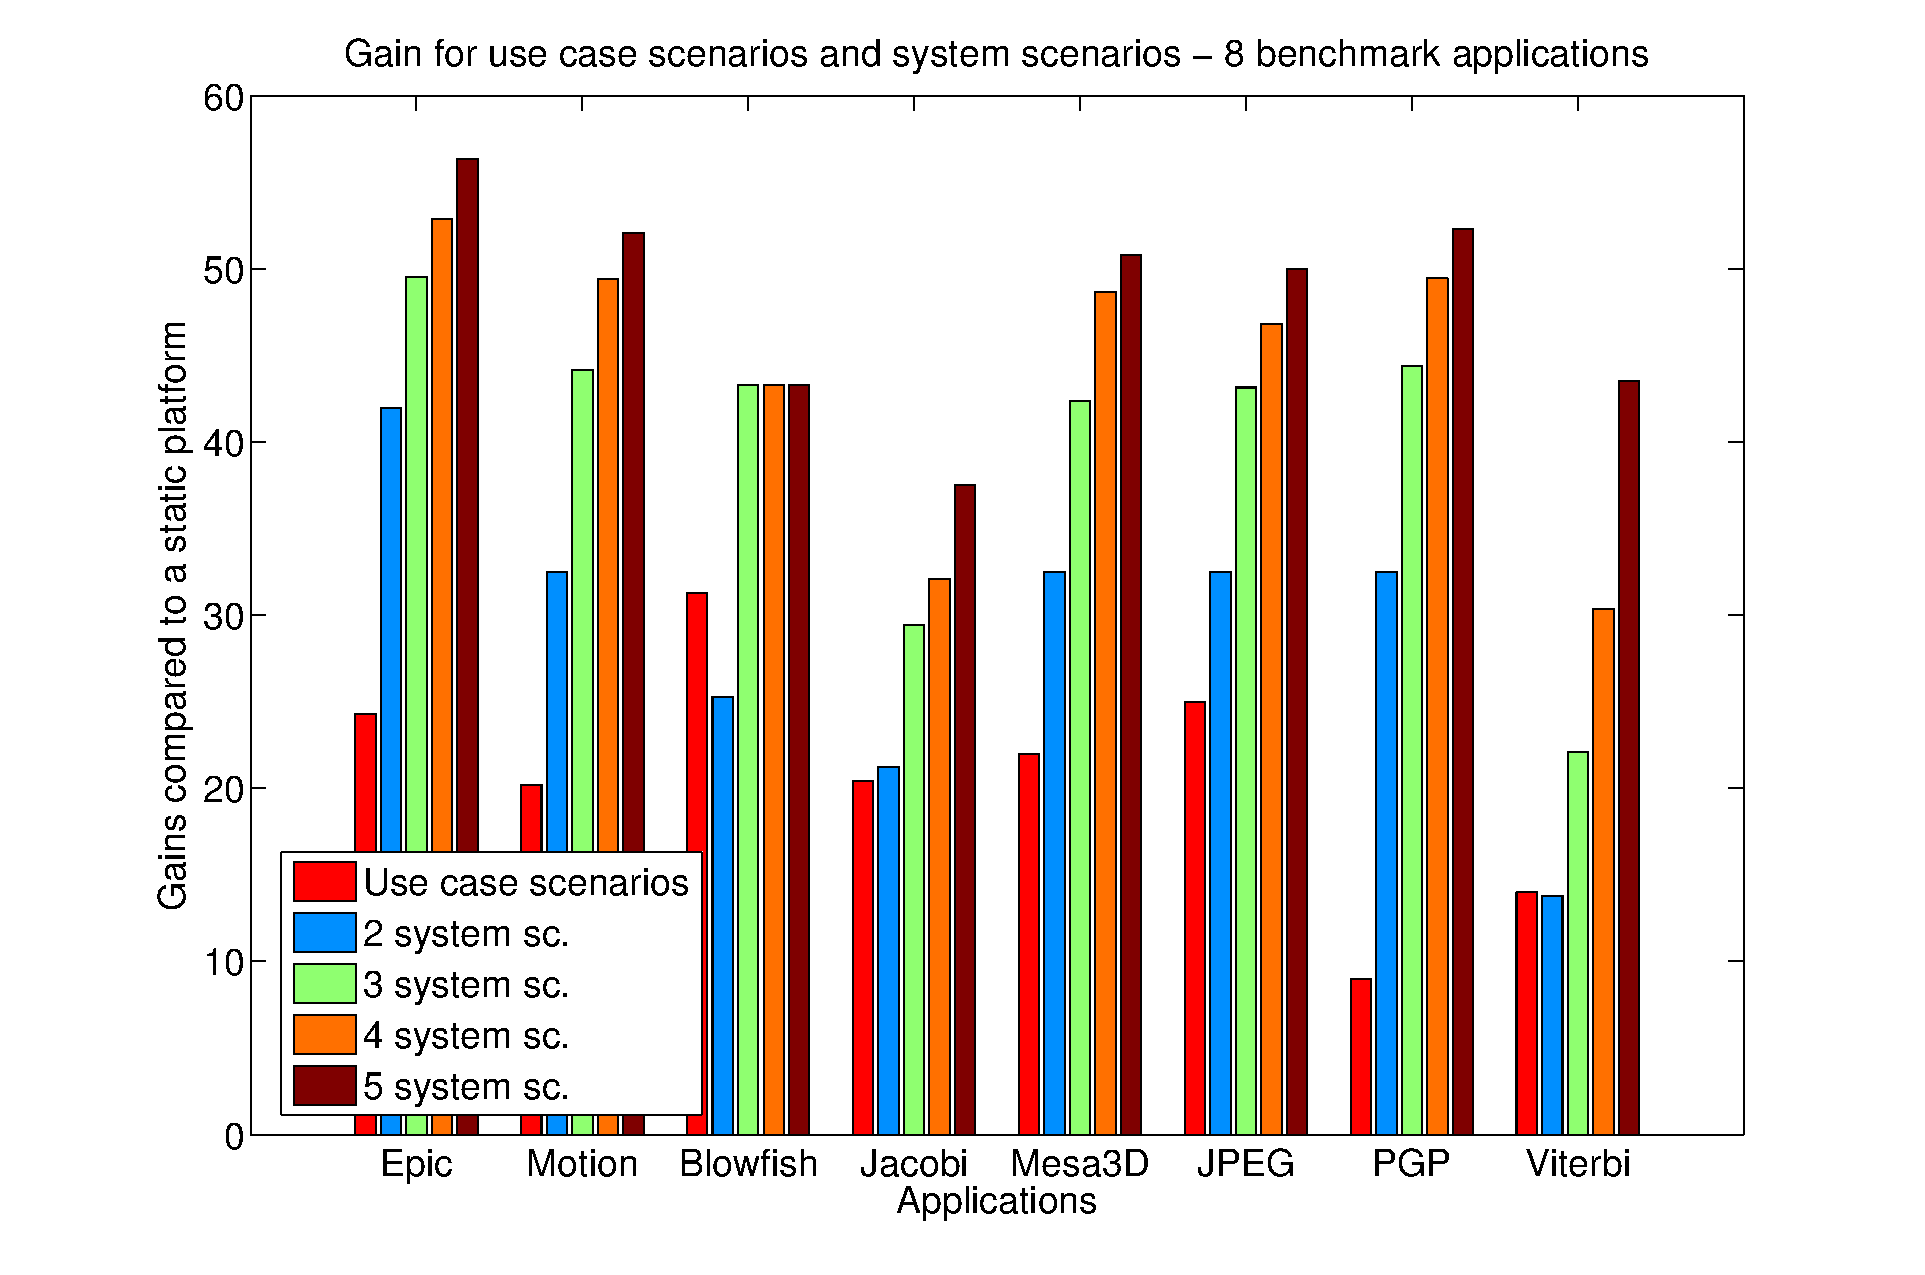
\includegraphics[width=\textwidth]{B/Images/usecase.pdf}
%\includegraphics{file=Images/usecase.eps, width=0.47\textwidth}
\caption{Energy gain for use case scenarios and system scenarios}
\label{fig:usecase}
\end{figure}

\section{Conclusion}
%\label{sec:conclusion}

The scope of this work is to apply the memory-aware system scenario methodology to a wide range of multimedia application and test its effectiveness based on an extensive memory energy model. The results demonstrate the effectiveness of the methodology reducing the memory energy consumption between 35\% and 55\%. 

\bibliographystyle{plain}
\bibliography{reference} 
\chapter{Exploration of energy efficient memory organizations for dynamic multimedia applications using system scenarios}
\label{DAES}

\begin{center}
Iason Filippopoulos, Francky Catthoor and Per Gunnar Kjeldsberg
\\
Design Automation for Embedded Systems
\\
Springer
\\
2014
\end{center}
\afterpage{\null\newpage}
\newpage

\vspace*{\fill}
\phantomsection
\section*{\hspace*{\fill} Abstract \hspace*{\fill}}
\addcontentsline{toc}{section}{Abstract}
We propose a memory-aware system scenario approach that exploits variations in memory needs during the lifetime of an application in order to optimize energy usage. 
Different system scenarios capture the application's different resource requirements that change dynamically at run-time. 
In addition to computational resources, the many possible memory platform configurations and data-to-memory assignments are important system scenario parameters. 
In this work we focus on clustering of different memory requirements into groups and presenting the system scenario generation in detail.
The clustering is a non-trivial problem due to the many different memory requirements, which leads to a very large exploration space.
An extended memory model is used as a practical enabler, in order to evaluate the methodology. 
The memory models include existing state-of-the-art memories, available from industry and academia, and we show how they are employed during the system design exploration phase. 
Both commercial SRAM and standard cell based memory models are explored in this study. 
The effectiveness of the proposed methodology is demonstrated and tested using a large set of multimedia benchmarks published in the Polybench, Mibench and Mediabench suites,
representative for the domain of multimedia applications.
Reduction in energy consumption in the memory subsystem ranges from 35\% to 55\% for the chosen set of benchmarks.
\vspace*{\fill}
\afterpage{\null\newpage}
\newpage

\section{Introduction}
\label{sec:introductionC}

Modern embedded systems are becoming more and more powerful as the semiconductor processing techniques keep increasing the number of transistors on a single chip. 
Consequently, demanding applications, e.g., in the signal processing and multimedia domains, can be executed on these devices \cite{narasinga}. 
On the other hand, the desired performance has to be delivered with minimum power consumption due to the limited energy available in mobile devices \cite{tcm}. 
System scenario methodologies propose the use of different platform configurations in order to exploit run-time variations in computational and memory needs often seen in such applications \cite{tcm}.

Platform reconfiguration is performed through tuning of different system parameters, also called system knobs. 
For the memory-aware system scenario methodology, a platform can be reconfigured through a number of potential knobs, each resulting in different performance and power consumption in the memory subsystem. 
Foremost, modern memories support different energy states, e.g., through power gating techniques and by switching to lower power modes when not accessed. 
The second platform knob is the assignment of data to the available memory banks.
The data assignment decisions affect both the energy per access for the mapped data, the data conflicts as a result of suboptimal assignment, and the number of active banks. 
In this work a reconfigurable memory platform is constructed using detailed memory models. 
This is followed by experiments with dynamic multimedia applications in order to study the effectiveness of the methodology.

The main contribution of the current work is the development of data variable \cite{Elena2012} based system scenarios.
Previous control variable based system scenarios \cite{Gheorghita2007} are unable to handle the fine-grain behavior of the studied multimedia applications due to their significant variation under different execution situations. 
Furthermore, compared with use case scenario approaches in which scenarios are generated based on a user's behavior \cite{usecase}, the system scenario methodology focuses on the behavior of the system to generate scenarios and can, therefore, fully exploit the detailed platform mapping information. 
Compared with previous work on system scenarios that has focused on the processing cores, the current work analyses the use of system scenarios on the memory organization. 
More specifically, this work focuses on the system scenario identification phase of the methodology.
The wide range of memory requirements, the amount of different cases, and the different frequency in which each case occurs, results in a very large exploration space.
Therefore, there is a need for developing an algorithmic approach that can efficiently tackle this problem.

Another significant contribution is the extensive number of benchmark applications on which the methodology is applied.
The chosen set is representative for the domain of multimedia applications.
Furthermore, we present a categorisation of applications based on their dynamic characteristics, also applicable to the entire multimedia domain. 
For the experimental needs of this work we present for the purpose sufficiently detailed and accurate  memory models, which are used for the system design exploration.
For the multimedia domain, the current work presents a comprehensive methodology for optimising energy consumption in the memory subsystem.

This article is organized as follows. 
Section~\ref{sec:motivationC} motivates the study of optimization of the memory organization. 
Section~\ref{sec:relatedC} surveys related work on system level memory exploration and on system scenario methodologies and compares it with the current work. 
Section~\ref{sec:methodologyC} presents the chosen methodology with main focus on the memory organization study. 
In Section~\ref{sec:platformC} the target platform is described accompanied by a detailed description of the employed memory models, while the multimedia benchmarks and their characteristics are analysed in Section~\ref{sec:applicationsC}. 
Results of applying the described methodology to the targeted applications are shown in Section~\ref{sec:resultsC}, while conclusions are drawn in Section~\ref{sec:conclusionC}. 

\section{Motivational Example}
\label{sec:motivationC}

A large number of papers have demonstrated the importance of the memory organization to the overall system energy consumption. 
As shown in \cite{Gonzalez1996} memory contributes around 40\% to the overall power consumption in general purpose systems. 
Especially for embedded systems, the memory subsystem accounts for up to 50\% of the overall energy consumption \cite{Che09} and the cycle-accurate simulator presented in \cite{Ben99} estimates that the energy expenditures in the memory subsystem range from 35\% up to 65\% for different architectures. 
The breakdown of power consumption for a recently implemented embedded system presented in \cite{Hul11} shows that the memory subsystem consumes more than 40\% of the leakage power on the platform. 
According to \cite{tcm}, conventional allocation and assignment of data done by regular compilers is suboptimal. 
Performance loss is caused by stalls for fetching data and data conflicts for different tasks, due to the limited size of memory and the competition between tasks. 

\begin{algorithm}
\caption{Motivational example of dynamic memory usage}
 \label{alg:motivation}
 \begin{algorithmic}[1]
	\WHILE{$image \ne EndOfDatabase$}
		\STATE $height \gets height(image)$
		\STATE $width \gets width(image)$
		\STATE $store(image[height][width])$
			\FOR{$i = 0 \to height$} 
				\FOR{$j = 0 \to width$} 
					\STATE $array[i][j] \gets func1(image[i][j])$
				\ENDFOR
			\ENDFOR
		\STATE $image \gets new.image$	
	\ENDWHILE
 \end{algorithmic}
\end{algorithm}

In addition, modern applications exhibit more and more dynamic behavior, which is reflected also in fluctuating memory requirements \cite{tcm}. 
Techniques have been developed in order to estimate the memory size requirements of applications in a systematic way \cite{Ang13}. 
The significant contribution that the memory subsystem has to the overall energy consumption of a system and the dynamic nature of many applications offer a strong motivation for the study and optimization of the memory organization in modern embedded devices.

To illustrate the sub-optimal conventional allocation and assignment of data, the simple example of Alg.~\ref{alg:motivation} is used. 
The kernel code of an image processing application continuously reads a sequence of images, saves each image in memory and performs function \textit{func1} on each pixel of the image. 
Arrays are typically used for storing the intermediate calculations in image processing applications, exemplified with the \textit{array} variable in the motivation example. 
The memory size used for the storage of each initial \textit{image} and the computed \textit{array} are determined by the dimensions of the input image and can be different for a series of input images. 
In a conventional assignment the highest values of \textit{height} and \textit{width} are identified and a static compiling results in allocation of the worst-case area for the \textit{array} variable. 
However, only a part of the allocated space is accessed during processing of smaller images. 

Assume for instance that we have two different image sizes, ImgA with L=H=1 and ImgB with L=H=2. 
That is, the size of ImgB is 4 $\times$ ImgA. 
Each pixel in each image is accessed once giving rise to N accesses to each ImgA and 4 $\times$ N accesses to each ImgB. 
Furthermore, in the input stream of images there are four times as many ImgA as ImgB. 
In our pool of alternative memories we have three memories with Size1 = ImgA, Size2  = 3 $\times$ ImgA, and Size 3 = 4 $\times$ ImgA (i.e., the size of ImgB). 
The energy cost of accessing a Size1 memory is 1E, while the average leakage energy in the time between the start of two accesses is 0.3E. 
The corresponding access/leakage numbers for Size2 and Size3 memories are 1.3E/0.9E and 1.5E/1.2E, respectively. 
The numbers reflects the fact that as a first order approximation access energy increases sub linearly with increased memory size, while leakage increases linearly with memory size. 
The total energy (access + leakage) during computations on four ImgA and one ImgB using only one memory of Size3 is:
\begin{align*}
4 \times N \times 1.5E + 4 \times N \times 1.5E + 8 \times N \times 1.2E = 21.6NE
\end{align*}
The same calculation using one memory of Size1 and one of Size2, in total the size of ImgB, is: 
\begin{align*}
& 4 \times N \times 1.0E + 1 \times N \times 1.0E + 3 \times N \times 1.3E \\
& + 4 \times N \times 0.3E + 4 \times N \times (0.3E + 0.9E) =  14.9NE
\end{align*}
giving a reduction in energy consumption of 31\%. 
These calculations are done with simplified assumptions regarding input data and memory models. 
The results in Section~\ref{sec:resultsC} show even larger gain with realistic dynamic applications, memory models and data.

\section{Related Work and Contribution Discussion}
\label{sec:relatedC}

%Many papers have focused on memory related optimisations, also in the presence of a partitioned and distributed memory organization with memory blocks of different sizes. 
%In \cite{Ben00b} authors present a methodology for automatic memory hierarchy generation that exploits memory access locality, while in \cite{Ben00c} they propose an algorithm for the automatic partitioning of on-chip SRAM in multiple banks. 
The memory allocation problem has been studied before. 
However, we extend state of the art by proposing a more generic approach, which is also suitable for applications with input driven dynamic behavior. 
The authors in \cite{Ben00b} present a methodology to generate a static application-specific memory hierarchy. 
Later, they extend their work in \cite{Ben00c} to a reconfigurable platform with multiple memory banks. 
However, our work differentiates by proposing a more generic and application agnostic methodology and employing the use of system scenarios, in order to efficiently handle a wider range of dynamic application characteristics. 

Several techniques for designing energy efficient memory architectures for embedded systems are presented in \cite{Mac02}. 
The current work differentiates by employing a platform that is reconfigurable at run-time. 
In \cite{Pgk01} a large number of data and memory optimisation techniques, that could be dependent or independent of a target platform, are discussed. 
Again, reconfigurable platforms are not considered.

Energy-aware assignment of data to memory banks for several task-sets based on the MediaBench suit of benchmarks is presented in \cite{Mar03}. 
Low energy multimedia applications are discussed also in \cite{Chu02} with focus on processing rather than the memory platform. 
Furthermore, both \cite{Mar03} and \cite{Chu02} base their analysis on use case situations and do not incorporate sufficient support for very dynamically behaving application codes. 
System scenarios alleviate this bottleneck and enable handling of such dynamic behavior. 
In addition, the current work explores the assignment of data to the memory and the effect of different assignment decisions on the overall energy consumption.

The authors in \cite{abraham1999automatic}, \cite{jacob1996analytical} and \cite{li1999hardware} present methodologies for designing memory hierarchies.
Design methods with main focus on the traffic and latencies in the memory architecture are presented in \cite{chen1999loop}, \cite{grun2000mist}, \cite{jantsch1994hardware} and \cite{passes1995multi}.
Improving memory energy efficiency based on a study of access patterns is discussed in \cite{kandemir2001improving}.
Application specific memory design is a research topic in \cite{schmit1997synthesis}, while memory design for multimedia applications is presented in \cite{oshima1997high}.
The current work differentiates by introducing the concept of system scenarios that supports the dynamic handling of application's requirements, although the data mapping is static inside each scenario. 

An overview of work on system scenario methodologies and their application are presented in \cite{Gheorghita2007}. 
In \cite{Fil12} extensions towards a memory-aware system scenario methodology are presented and demonstrated using theoretical memory models and two target applications. 
This work is an extension both in complexity and accuracy of the considered memory library and on the number of target applications. 

Furthermore, the majority of the published work focus on control variables for system scenario prediction and selection. 
Control variables can take a relatively small set of different values and thus can be fully explored. However, the use of data variables \cite{Elena2010} is required by many dynamic systems including the majority of multimedia applications. 
The range of possible values for data variables is wider and makes full exploration impossible. 

Authors in \cite{Pal06} present a technique to optimise memory accesses for input data dependent applications by duplicating and optimising the code for different execution paths of a control flow graph (CFG). 
One path or a group of paths in a CFG form a scenario and its memory accesses are optimised using global loop transformations (GLT). 
Apart from if-statement evaluations that define different execution paths, they extend their technique to include while loops with variable trip count in \cite{Pal06b}. 
A heuristic to perform efficient grouping of execution paths for scenario creation is analysed in \cite{Pal07}. 
Our work extends the existing solutions towards exploiting the presence of a distributed memory organization with reconfiguration possibilities.

Reconfigurable hardware for embedded systems, including the memory architecture, is a topic of active research. 
An extensive overview of current approaches is found in \cite{Garcia}. 
The approach presented in this paper differentiates by focusing on the data-to-memory assignment aspects in the presence of a platform with dynamically configurable memory blocks. 
Moreover, many methods for source code transformations, and especially loop transformations, have been proposed in the memory management context. 
These methods are fully complementary to our focus on data-to-memory assignment and should be performed prior to our step. 

\section{Data Variable Based Memory-Aware System Scenario Methodology}
\label{sec:methodologyC}

The memory-aware system scenario methodology is based on the observation that the memory subsystem requirements at run-time vary significantly due to dynamic variations of memory needs in the application code. 
Most existing design methodologies define the memory requirements as that of the most demanding task and tune the system in order to meet its needs \cite{tcm}. 
Obviously, this approach leads to unused memory area for tasks with lower memory requirements, since those tasks could meet their needs using fewer resources and consequently consuming less energy. 
Another source of energy waste in the memory system is caused by data conflicts due to misplaced data. 
Replacement of old data and fetching of new data is both time and energy consuming and should therefore be avoided. 
Handling of data conflicts is also part of a memory-aware system scenario methodology.

Designing with system scenarios is workload adaptive and offers different configurations of the platform and the freedom of switching to the most efficient scenario at run-time. 
A system scenario is a configuration of the system that combines similar run-time situations (RTSs). 
An RTS consists of a running instance of a task and its corresponding cost (e.g., energy consumption) and one complete run of the application on the target platform represents a sequence of RTSs \cite{Elena2010}. 
The system is configured to meet the cost requirements of an RTS by choosing the appropriate system scenario, which is the one that satisfies the requirements using minimal power. 
In the following subsections, the different steps of the memory-aware system scenario methodology are outlined. 

The system scenario methodology follows a two stage exploration, namely design-time and run-time stages, as described in \cite{Gheorghita2007}. 
This splitting is also employed in the memory-aware extension of the methodology. 
The two stage exploration is chosen because it reduces run-time overhead while preserving an important degree of freedom for run-time configuration \cite{tcm}. 
The application is analysed at design-time and different execution paths causing variations in memory demands are identified. 
This procedure, which is time consuming and as a result can be performed only during the design phase, will result in a grey-box model representation of the application. 
The grey-box model hides all static and deterministic parts of the application, instead only providing their related memory costs to the system designer.
Parts of the application code that are non-deterministic in terms of memory usage are directly available to the system designer \cite{graybox}. 


\subsection{Design-time Profiling Based on Data Variables}

\begin{figure}
\centering
\includegraphics[width=0.75\textwidth]{C/profiling2.pdf}
\caption{Profiling results based on application code and input data}
\label{fig:profilingC}
\end{figure}

Application profiling is performed at design-time for a wide range of inputs. 
The analysis focuses on the allocated memory size during execution and on access pattern variations. 
Techniques described in \cite{Ang13b} are, e.g., used in order to extract the access scheme through analysis of array iteration spaces.  

The profiling stage is depicted in Fig.~\ref{fig:profilingC} and consists of running the application code with suitable input data often found in a database, in order to produce profiling results. 
The results shown here are limited for demonstrational purposes. 
A real application would have thousands or millions of profiling samples. 
The profiling reveals parts of the application code with high memory activity and with varying memory access intensity, which possibly depends on input data variables. 
Because of this behavior, a static study of the application code alone is insufficient since the target applications for this methodology have non-deterministic behavior that is driven by input.

Profiling results provided to the designer include complete information about allocated memory size values together with the number of occurrences and duration for each of these memory size values. 
Moreover, correlation between input data variable values and the resulting memory behavior can possibly be observed. This information is useful for the clustering step that follows. 
Profiling also reveals the worst case memory usage for a given set of inputs. 
The memory usage is measured using techniques presented in \cite{Ang13b}, in which authors compute the minimum amount of memory resources required to store the elements of an application. 

In Fig.~\ref{fig:profilingC} the profiled applications are two image related multimedia benchmarks and the input database should consist of a variety of images. 
The memory requirements in each case are driven by the current input image size, which is classified as a data variable due to the wide range of its possible values. 
Depending on the application the whole image or a region of interest is processed. 
Other applications have other input variables deciding the memory requirement dynamism, e.g., the channel SNR level in the case of an encoding/decoding application.

The input data used for profiling are generated based on realistic assumptions for each of the chosen benchmarks. 
Each application is studied and based on its functionality, a range of rational inputs are developed. 
In addition, example inputs are available for most of the studied benchmark applications. 
The choice of common and open-source benchmarks provides us the opportunity to find inputs publicly available. 
Based on the collected information, we define the range of realistic inputs and we generate a random set on inputs within these limits. 
For example, the bibliography provides information for the real SNR levels and the constraint length of the Viterbi encoder for each level, in order to achieve a  successful communication. 
For profiling, we generate randomly a set of SNR levels that cover this whole range. 
Similar technique is used for the applications that use an image as an input. 
First, we explore the sizes of images commonly used to define the minimum and the maximum size and then we randomly generate a set of image sizes within the size limits. 
For the random generation of inputs, we assume the same probability for each situation, because there is no information available regarding the frequency of each input. 
As a result the frequency of each input is random. 

\subsection{Design-time System Scenario Identification Based on Data Variables}

\begin{figure}
\centering
\includegraphics[width=0.75\textwidth]{C/1Dclustering.pdf}
\caption{Clustering of profiling results into three (a) or five (b) system scenarios}
\label{fig:clusteringC}
\end{figure}

The next step is the clustering of the profiled memory sizes into groups with similar characteristics. 
This is referred to as system scenario identification. 
Clustering is necessary, because it will be extremely costly to have a different scenario for every possible size, due to the number of memories needed. 
Clustering neighbouring RTSs is a rational choice, because two instances with similar memory needs have similar energy consumption. 

In Fig.~\ref{fig:clusteringC} the clustering of the previously profiled information is presented. 
The clustering of RTSs is based both on their distance on the memory size axis and the frequency of their occurrence. 
Consequently, the memory size is split unevenly with more frequent RTSs having a shorter memory size range. 
In the case of a clustering to three system scenarios the space is divided in the three differently coloured hashed areas depicted in Fig.~\ref{fig:clusteringC}(a). 
Due to the higher frequency of RTSs in the yellow hashed area, that system scenario has a shorter range compared with its neighbouring scenarios. 
Such clustering is better than an even splitting because the energy cost of each system scenario is defined by the upper size limit, as each scenario should support all RTSs within its range. 
Consequently the overhead for the RTSs in the yellow area is lower compared to the overhead in the two other areas.

The same principle applies also when the number of system scenarios is increased to five, as depicted in Fig.~\ref{fig:clusteringC}(b). 
The frequency sensitive clustering results in two short system scenarios that contain four RTSs each and three wider system scenarios with lower numbers of RTSs. 
The number of system scenarios should be limited mainly due to two factors. 
First, implementation of a high number of system scenarios in a memory platform is more difficult and complex. 
Second, the switching between the different scenarios involves an energy penalty that could become significant when the switching takes place frequently.

The memory size and the frequency of each RTS are not the only two parameters that should be taken into consideration during the system scenario identification. 
The memory size of each RTS results in a different energy cost depending on the way it is mapped into memory. 
The impact of the different assignment possibilities is included into the clustering by introduction of energy as a cost metric. 
The energy cost for each RTS is calculated using a reference platform with one to N
memory banks. 
Increasing the number of memory banks results in lower energy per access since the most accessed elements can be assigned to smaller and more energy efficient banks. Unused banks can be switched off.

In the system scenario methodology, Pareto curves are used to capture alternative system configurations within a scenario \cite{tcm}. 
In our work, a Pareto space is used for clustering that also includes the energy cost metric. 
For each RTS all different assignment options on alternative platform configurations are studied. 
Memory platform knobs are different sets of memory banks that are turned on and off.
A Pareto curve is constructed for each RTS that contains the optimal assignment for each platform configuration. 
Hence, suboptimal assignments and assignments that result in conflicts are not included in the Pareto curve. 
In Fig.~\ref{fig:paretoC} four Pareto curves, each corresponding to a different RTS, are shown together with energy cost levels corresponding to different platform configuration and data-to-memory assignment decisions. 
Three non-optimal mappings are also shown in Fig.~\ref{fig:paretoC} for illustration. 
They are not part of the Pareto curve and consequently not included in the generation of scenarios. 
Pareto curves are clustered into three different system scenarios based again both on their memory size differences and frequency of occurrence. 
Clustering of RTSs using Pareto curves is more accurate compared to the clustering depicted in Fig.~\ref{fig:clusteringC}, as it includes data-to-memory assignment options in the exploration. 

\begin{figure}
\centering
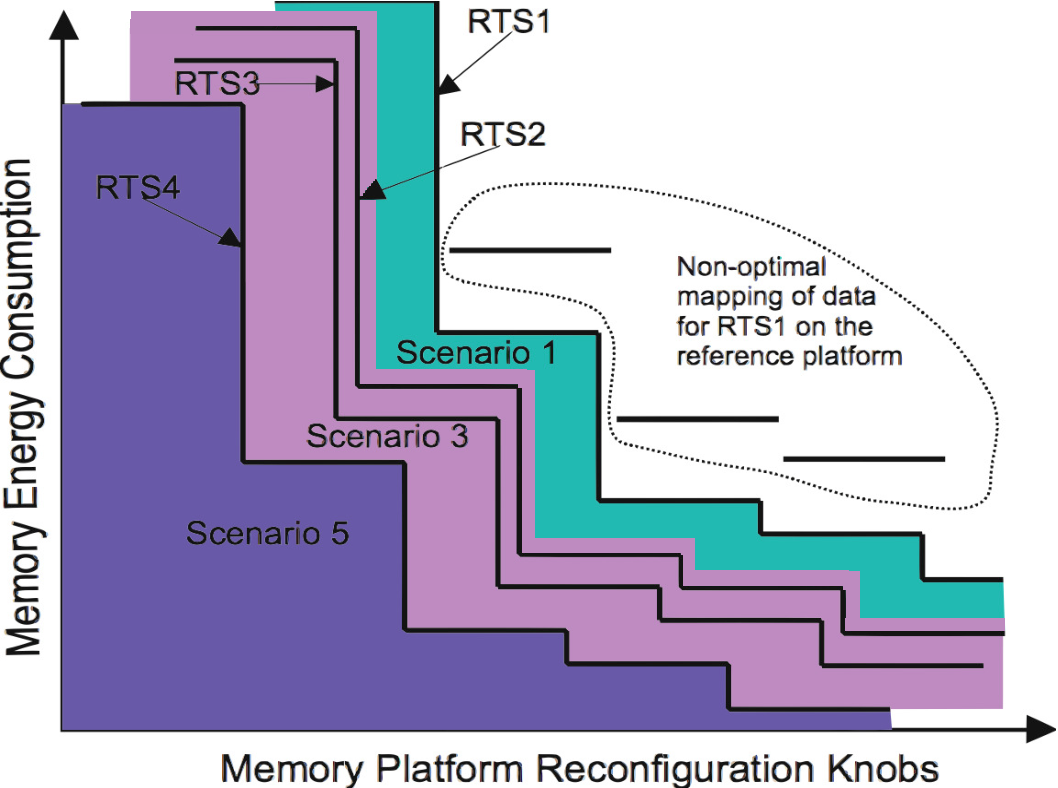
\includegraphics[width=0.75\textwidth]{C/2D.pdf}
\caption{Clustering of Pareto curves}
\label{fig:paretoC}
\end{figure}

The system scenario identification step includes the selection of the data variables that determine the active system scenario. 
This can be achieved by careful study of the application code, combined with the application's data input.
The variable selection is done before clustering of RTSs into scenarios.
For the choice of identification variables, there is a trade-off between the complexity and the accuracy of the scenario detection step.
On one hand, if the identification is done using a group of complex variables and their correlation, there is a number of calculations needed in order to predict the active scenario. 
On the other hand, if the value of a single variable is monitored for scenario identification, the scenario detection is straightforward.
Obviously, the accuracy of the scenario detection is higher on the first case, while the computational needs for scenario detection are lower on the second case.
In other words, the more accurate scenario detection, the more resources are used by the run-time manager for detection.
In our case the grey-box model reveals only the code parts that will influence memory usage, so that data variables deciding memory space changes can be identified. 
An example of this is a non static variable that influences the number of iterations for a loop that performs one memory allocation at each iteration. 
In the depicted example the system scenario detection data variable is the input image height and width values. 
Moreover, the designer should look for a correlation between input values and the corresponding cost. 
This information will be useful in the following steps of the methodology \cite{tcm}.

\subsection{Run-time System Scenario Detection and Switching Based on Data Variables}

Switching decisions are taken at run-time by the run-time manager. 
In this work, we use a simple and straightforward switching approach.
Memory models provide the necessary information for the switching decision, namely the energy and the time penalty for switching between stages.
The switching step consists of all platform configuration decisions that can be made at run-time, e.g., frequency/voltage scaling, changing the power mode of memory units, including turning them off, and reassignment of data to memory units. 
Switching takes place when the switching cost is lower than the energy gains achieved by switching. 

In more detail, the switching mechanism implemented by the run-time manager includes the following actions: 
\begin{enumerate}
\item Calculation of the energy consumption by processing the next input on the currently active scenario (E1).
\item Calculation of the energy consumption by processing the next input on its most energy efficient scenario (E2).
\item Calculation of the energy penalty for switching the needed memory banks to the configuration of the most efficient scenario (E3).
\item Evaluation of the expression: E1 \textgreater  E2 + E3. If the energy cost of the current configuration (E1) is greater than the combined cost of the new configuration and the required switching (E2 + E3), then the decision is to switch. Otherwise, the switching decision is negative and the system stays on the currently running configuration
\item Switching of the platform to its new configuration. The memory banks switch to the appropriate state, which is defined by the chosen scenario. 
\end{enumerate}
% the run-time manager compares the memory energy consumption of executing the next task in the current active system scenario with the energy consumption of execution with the optimal system scenario. 
%If the difference is greater than the switching cost, then scenario switching is performed \cite{tcm}. 
Switching costs are defined by the platform and include all memory energy penalties for run-time reconfigurations of the platform, e.g., extra energy needed to change state of a memory unit.

The run-time manager is minimal, resulting in a very small overhead, and is complementary to an operating system (OS), if such is available on the platform. 
In the presence of an embedded OS, the OS needs to start the runtime manager and grant it access to system reconfiguration calls. 
In both cases, when the run-time manager is active, it performs a few simple steps with minimal system performance overhead. 
In more detail, the run-time manages checks the current state of the monitored identification variable(s), determine the next scenario based on this value and decides whether switching should be performed. 
The corresponding scenario for a given value of the identification variable is a simple look-up, because all the analysis has been performed at design-time. 
The hardware configuration for the active scenario is also explored at design-time and the run-time manager is aware of the required changes. 
In our approach no need is present for modifications of the application code.
Instead, we add the above mentioned changes in the middleware layer. 
That has the additional advantage that the run-time manager is reusable across several tasks/processes running at the application layer on top of this shared middleware. 
The application data are stored and accessed the same way at the application level. 
The difference with the proposed approach is the size and the state of the memory bank that the data are stored in. 
The application is unaware of the exact way the data is stored and accessed and the methodology ensures that the accessed addresses in the application code always corresponds to an active bank.

\begin{figure}
\centering
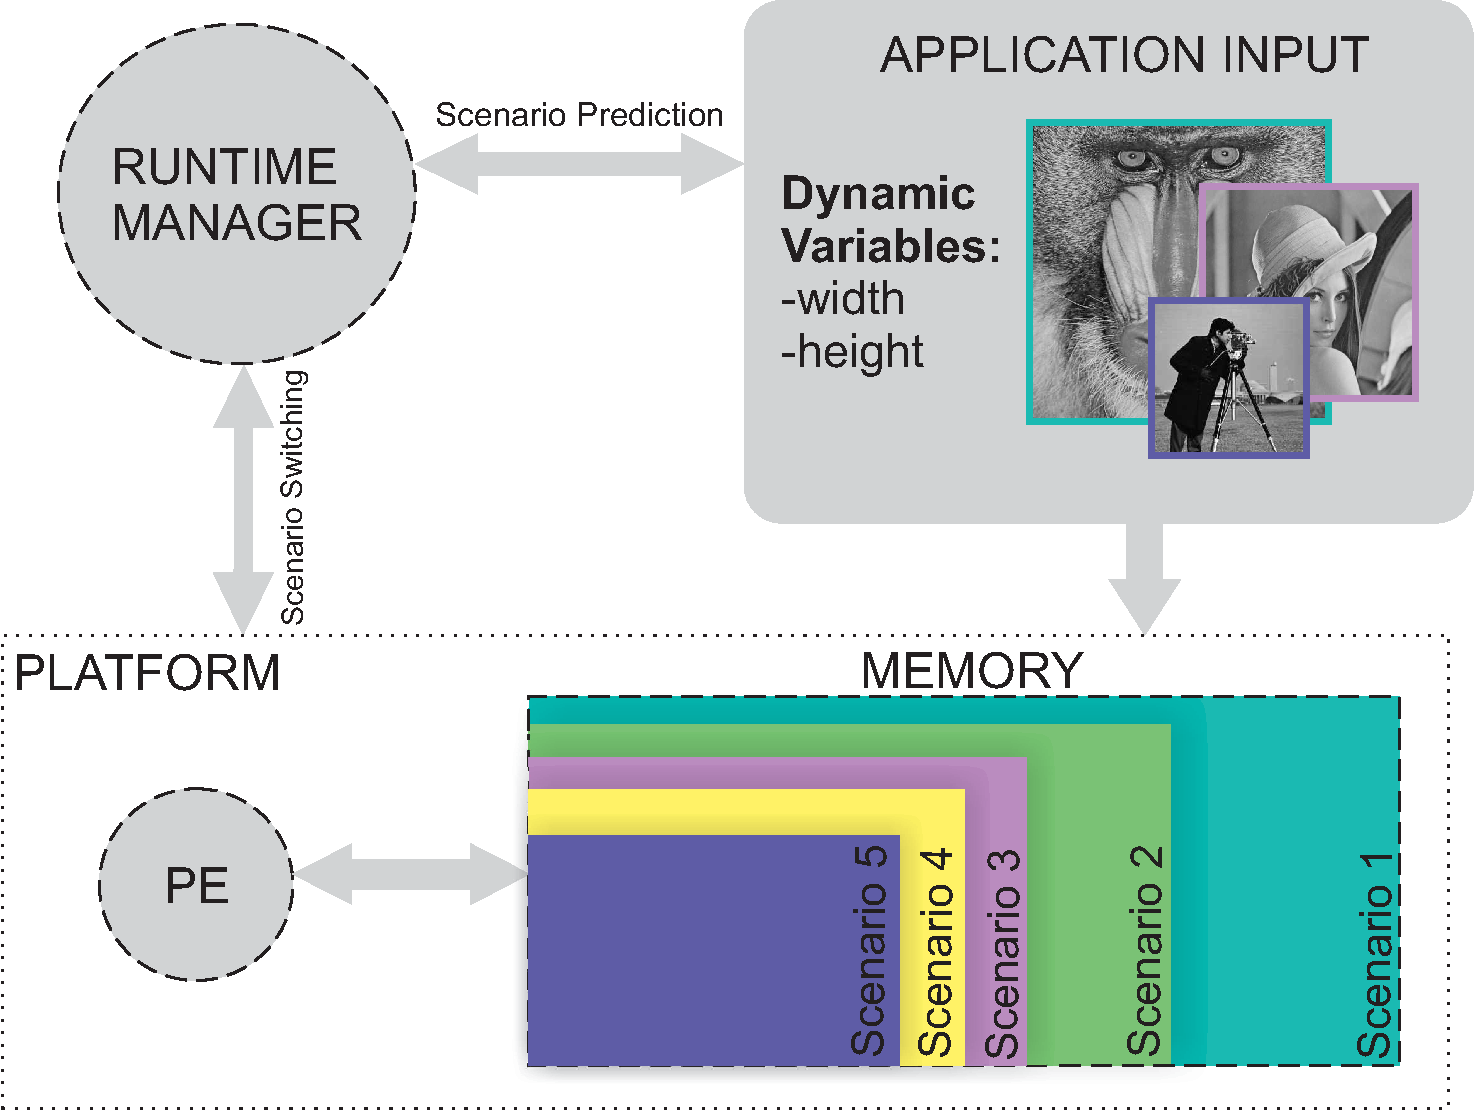
\includegraphics[width=0.75\textwidth]{C/switching.pdf}
\caption{Run-time system scenario detection and switching based on the current input}
\label{fig:runtimeC}
\end{figure}

In Fig.~\ref{fig:runtimeC} an example of the run-time phase of the methodology is depicted. 
The run-time manager identifies the size of the image that will be processed and reconfigures the memory subsystem on the platform, if needed, by increasing or decreasing the available memory size. 
The reconfiguration options are effected by platform hardware limitations. 
The image size is in this case the data variable monitored in order to detect the system scenario and the need for switching.

\section{Target Platform and Energy Models}
\label{sec:platformC}

Selection of target platform is an important aspect of the memory-aware system scenario methodology. 
The key feature needed in the platform architecture is the ability to efficiently support different memory sizes that correspond to the system scenarios generated by the methodology. 
Execution of different system scenarios then leads to different energy costs, as each configuration of the platform results in a specific memory energy consumption. 
The dynamic memory platform is achieved by organising the memory area in a varying number of banks that can be switched between different energy states. 

\subsection{Target Memory Platform Architecture}

In this work, a clustered memory organization with up to five memory banks of varying sizes is explored. 
The limitation in the number of memory banks is necessary in order to keep the interconnection cost between the processing element (PE) and the memories constant through exploration of different architectures. 

For more complex architectures the interconnection cost should be considered and analysed separately for accurate results. 
Although power gating can be applied to the bus when only a part of a longer bus is needed, an accurate model of the memory wrapper and interconnection must developed, which is beyond the scope of the current work. 

\begin{figure}
\centering
\includegraphics[width=0.75\textwidth]{C/platform.pdf}
\caption{Alternative memory platforms with varying number of banks}
\label{fig:platformC}
\end{figure}

%Minor revision comment 2
Some examples of alternative memory platforms that can be used for exploration is shown in Fig.~\ref{fig:platformC}. 
Point-to-point connections with negligible interconnect costs between elements are assumed for up to five memory banks. 
The decision to use memory banks with varying sizes on the clustered memory organization increases the reconfiguration options and consequently the potential energy gains. 
In general, smaller memories are more energy efficient compared to larger memories banks. 
However, in some cases large memory banks are needed in order to fit the application data without the need for too many small memories causing complex interconnects. 
The goal is to use the most energy efficient banks to store the most frequently used data. 
The calculations needed for enabling the minimum number of banks is simple, given the application requirements for the current input and the sizes of the five memory banks.

\subsection{Models of Different Memory Types}
The dynamic memory organization is constructed using commercially available SRAM memory models (MM) \nomenclature{MM}{memory macros}.
For those models delay and energy numbers are derived from a commercial memory compiler.
In addition, experimental standard cell-based memories (SCMEM) \cite{Mei11}  are  considered for smaller memories due to their energy and area efficiency for reasonably small storage capacities, as argued in \cite{Mei10}. 
The standard cell-based memories are synthesized using Cadence RTL \nomenclature{RTL}{register transfer language} compiler for TSMC 40nm standard library. 
Afterwords, power simulations on the synthesized design are carried out using Synopsys PrimeTime, in order to obtain energy numbers.
Both MMs and SCMEMs can operate under a wide range of supply voltages, thus support different operating modes that provide an important exploration space.
\begin{itemize}
\item Active mode: The normal operation mode, in which the memory can be accessed at the maximum supported speed. The supply voltage is 1.1V. 
The dynamic and leakage power are higher compared to the other modes.
Only on active mode the data are accessible without time penalties, in contrast to light and deep sleep modes.
In this work all the memory accesses are performed in active mode. 
\item Light sleep mode: The supply voltage in this mode is lower than active with values around 0.7V. 
The access time of the memory is significantly higher than the access time in active mode. 
Switching to active mode can be performed with a negligible energy penalty and a small time penalty of a few clock cycles (less than 10). 
Data is retained.  
\item Deep sleep mode: The supply voltage is set to the lowest possible value that can be used without loss of data. 
This voltage threshold is expected to be lower for SCMEMs than MM models and can be as low as 0.3V. 
The number of clock cycles needed for switching to active mode is higher compared to sleep mode, typically in the range of 20 to 50 clock cycles depending on the clock speed. 
Consequently, the speed of the PE and the real-time constrains of the applications has to be taken into consideration when choosing light or deep sleep mode at a specific time.  
\item Shut down mode: Power-gating techniques are used to achieve near zero leakage power. 
Stored data is lost. 
The switch to active mode requires substantially more energy and time. 
However, switching unused memories to this mode, providing that their data are not needed in the future, results in substantial energy savings.
\end{itemize}  

%Minor revision comment 1
The exploration includes memories with 4 energy modes in contrast to a more conservative approach that assumes only on and off states. 
This is in line with is modern energy efficient memories that tend to support an increasing number of energy modes as a feature. 
The methodology is still applicable to a memory organization that supports only two modes, but the intention of this work is to explore the state of the art memory technologies.
The policy for switching between the modes depends on the reuse of the stored data, which  depends on the nature of the target application.
The switching policy is determined by examining the following condition for the stored data in a memory bank:
\begin{itemize}
\item If the data is currently under processing, then the only acceptable mode is the active mode.
\item If the data is not accessed, but will be needed in the near future, then the light or deep sleep mode should be chosen.
\item If the processing of the data is completed and the application is not accessing them again, the shut-down mode is the optimal solution.
\end{itemize}

Applications that perform calculations on a set of input data to produce a result and never re-access the initial data, normally only use two modes.
The need for more energy modes arises from the fact that many applications re-access the initial data or some intermediate results.
Thus, the runtime manager chooses a sleep mode that reduces the leakage power, but retains the data for future use. 
%Another example of efficient usage of different modes is the parallel processing of data stored in multiple banks by an application.
%In this case, if there is a time consuming processing in one bank (i.e. a moving object is found in a part of the image), there is an opportunity to switch some banks in sleep mode while waiting.

The necessary energy/power information is available to the system designer and relative values for a subset of the used sizes in the current work are presented in Tab.~\ref{tab:rel1} and in Tab.~\ref{tab:rel2}. 
It shows that the choice of memory units has an important impact on the energy consumption. 
Moreover, different decisions have to be made based on the dominance of dynamic or leakage energy in a specific application. 
In the current work memory architectures with 1 to 5 memory units  of different sizes are explored and the optimal configuration is chosen. 
The methodology is in general not restricted to specific memory types or benchmarks and can handle more complex hierarchical memory architectures and applications. 
However, in this study the chosen applications have a relatively small memory space requirement limited to around 100KB, which is the case for many applications run on modern embedded systems. 

\begin{table}
	\caption{Relative dynamic energy for a range of memories with varying capacity and type}
	\label{tab:rel1}
	\begin{tabular}{|c|c|c|c|c|c|}
		\hline
		\multirow{2}{*}{\textbf{Type}} & \textbf{Lines x} & \multicolumn{2}{c|}{\textbf{Dynamic Energy [J]}} & \multicolumn{2}{c|}{Switching to Active from} \\ \cline{3-4}
		& \textbf{wordlength} & Read & Write  & Deep[uJ] & Light[uJ]\\ 
		\hline 
		MM & 32 x 8 &  $ 4.18 \times 10^{-8} $ &  $ 3.24 \times 10^{-8} $ & 0.223 &  0.031 \\ 
		\hline
		MM & 32 x 16 & $  6.79 \times 10^{-8} $ &  $ 5.89 \times 10^{-8} $ & 0.223 &  0.031\\ 
		\hline
		MM & 32 x 128 & $  4.33 \times 10^{-7} $ &  $ 4.31 \times 10^{-7} $ & 1.42 & 0.168\\ 
		\hline
		MM & 256 x 128 & $  4.48 \times 10^{-7} $ &  $ 4.60 \times 10^{-7} $ & 1.70 &  0.171\\ 
		\hline
		MM & 1024 x 128 & $  5.11 \times 10^{-7} $ &  $ 5.75 \times 10^{-7} $ & 2.81 & 0.179\\ 
		\hline
		MM & 4096 x 128 & $  9.60 \times 10^{-7} $ &  $ 4.57 \times 10^{-7} $ & 9.01 & 0.457\\ 
		\hline
		SCMEM & 128 x 128 & $  2.5 \times 10^{-7} $ &  $ 0.8 \times 10^{-8} $ & 1.51 &  0.045\\ 
		\hline
		SCMEM & 1024 x 8 & $  1.7 \times 10^{-8} $ &  $ 0.6 \times 10^{-8} $ & 0.325 &  0.021\\ 
		\hline
	\end{tabular}
\end{table}

\begin{table}
	\caption{Relative static power for a range of memories with varying capacity and type}
	\label{tab:rel2}
	\begin{tabular}{|c|c|c|c|c|c|}
		\hline
		\multirow{2}{*}{\textbf{Type}} & \textbf{Lines x} & \multicolumn{4}{c|}{\textbf{Static Leakage Power per Mode[W]}} \\ \cline{3-6}
		& \textbf{wordlength} & Active & Light-sleep & Deep-sleep & Shut-down\\ 
		\hline 
		MM & 32 x 8 & 0.132 & 0.125 & 0.063 & 0.0016\\ 
		\hline
		MM & 32 x 16 & 0.134 & 0.127 & 0.064 & 0.0022\\ 
		\hline
		MM & 32 x 128 & 0.171 & 0.160 & 0.083 & 0.0112\\ 
		\hline
		MM & 256 x 128 & 0.207 & 0.184 & 0.104 & 0.0293\\ 
		\hline
		MM & 1024 x 128 & 0.349 & 0.283 & 0.189 & 0.102\\ 
		\hline
		MM & 4096 x 128 & 0.95 & 0.708 & 0.544 & 0.396\\ 
		\hline
		SCMEM & 128 x 128 & 0.083 & 0.057 & 0.027 & 0.0022\\ 
		\hline
		SCMEM & 1024 x 8 & 0.042 &
		 0.028 & 0.014 & 0.0011\\ 
		\hline
	\end{tabular}
\end{table}

\subsection{Total Energy Consumption Calculation}
Both the dynamic and the static energy consumed in the memory subsystem is included in the calculations.
The overall energy consumption for each configuration is calculated using a detailed formula, as can be seen in Eq.\ref{eq:energyC}. 
All the important transactions on the platform that contribute to the overall energy are included, in order to achieve as accurate results as possible. In particular:
\begin{itemize}
\item $N_{rd}$ is the number of read accesses
\item $E_{Read}$ is the energy per read
\item $N_{wr}$ is the number of write accesses 
\item $E_{Write}$ is the energy per write 
\item T is the execution time of the application
\item $T_{LightSleep}$, $T_{DeepSleep}$ and $T_{ShutDown}$ are the times spent in light sleep, deep sleep and shut down states respectively
\item $P_{leak_{Active}}$ is the leakage power in active mode 
\item $P_{leak_{LightSleep}}$, $P_{leak_{DeepSleep}}$ and $P_{leak_{Shutdown}}$ are the leakage power values in light sleep, deep sleep and shut down modes with different values corresponding to each mode 
\item $N_{SWLight}$, $N_{SWDeep}$ and $N_{SWShutDown}$ are the number of transitions from each retention state to active state
\item $E_{LightSleep \: to \: Active}$, $E_{DeepSleep \: to \: Active}$ and $E_{ShutDown \: to \: Active}$  are the energy penalties for each transition respectively.
\end{itemize}
\setlength{\arraycolsep}{0.0em}
\begin{eqnarray}
\label{eq:energyC}
 E &{}= {}&\sum\limits_{memories}^{all}  ( N_{rd} \times E_{Read} \nonumber\\
		&&+ N_{wr} \times E_{Write} \nonumber\\
		&&+ (T - T_{LightSleep} - T_{DeepSleep} - T_{ShutDown}) \times P_{leak_{Active}} \nonumber\\
		&&+ T_{LightSleep} \times P_{leak_{LightSleep}} \nonumber\\
		&&+ T_{DeepSleep} \times P_{leak_{DeepSleep}} \nonumber\\
		&&+ T_{ShutDown} \times P_{leak_{ShutDown}} \nonumber\\ 
		&& + N_{SWLight} \times E_{LightSleep \: to \: Active} \nonumber\\
		&& + N_{SWDeep} \times E_{DeepSleep \: to \: Active} \nonumber\\
		&& + N_{SWShutDown} \times E_{ShutDown \: to \: Active} ) \nonumber\\
\end{eqnarray}
\setlength{\arraycolsep}{5pt}
The overall energy consumption is given after calculating the energy for each memory bank. 
The execution time of the application is needed to calculate the leakage time. 
It can be found by executing the application on a reference embedded processor. 
The simulator described in \cite{Gem5} is chosen to calculate execution time for the chosen applications in this work. 
The processor is assumed to be running continuously, accepting new input data as soon as computations on the previous data set has been finished. 
Memory sleep times are hence only caused by data dependent dynamic behavior.

\subsection{Memory Architecture Exploration}

The exploration of alternative memory platforms is performed using the steps described in Alg.~\ref{alg:clusteringC}. 
The exploration is performed at system scenario identification phase, after the profiling of RTSs.
All potentially energy efficient configurations are tested for a given number of scenarios and the sequence of RTSs of the application.
First, a database with all the memory models that are available to the system designer is imported.
The memory database can afterwards be pruned to reduce the complexity of the exploration, as explained in the following paragraph. 
After the optional pruning, all possible configurations for a given number of memory banks are constructed. 
The only requirement in order to keep a configuration for further investigation is that the combined size of all banks should satisfy the storage requirements of the most demanding RTS. 
Then, each configuration is tested for the sequence of RTSs and the one that minimizes Eq.\ref{eq:energyC} is chosen as the most energy efficient for this number of scenarios (i.e., number of banks). 

\begin{algorithm}
\caption{Memory organization exploration steps}
 \label{alg:clusteringC}
 \begin{algorithmic}[1]
		\STATE $RTSset \gets$ storage requirement for each RTS
		\STATE $Database \gets $ extensive memory database
		\STATE \textbf{\textit{//Database pruning:}} 
		\FOR {all relevant memory sizes}
		\STATE  pick memory models from $Database$ according to application characteristics
		%\FOR{$mem.size = min(Database) \to max(Database)$}
		%	\STATE $optimal.read(mem.size) \gets$ find model with the lowest read
			%\STATE $optimal.write(mem.size) \gets$ find model with the lowest write
			%\STATE $optimal.leakage(mem.size) \gets$ find model with the lowest leakage
		\ENDFOR	 
		\STATE $m \gets $ number of memory models in pruned $Database$
		\STATE $N \gets $ number of scenarios (up to 5 in this work)
		\STATE \textbf{\textit{//Exploration of memory organizations:}} 
			\FOR{$n = 1 \to N$}
				\STATE $k \gets$ combination of $n$ banks out of a set of $m$ memories  
				\FOR{all generated k combinations}
				\IF{$\sum_{1}^{n} size(bank) \geq  size(max(RTS))$} 
				\STATE \textbf{\textit{//Select configuration that minimizes Eq.\ref{eq:energyC}}} 
					\STATE{$Ecurrent \gets $ Energy given by Eq.\ref{eq:energyC} for current combination}
					\IF{$Eminimum > Ecurrent$}
						\STATE{$Eminimum \gets  Ecurrent$}
						%\STATE{Keep the current configuration as the most energy efficient}
					\ENDIF	
				\ENDIF
				\ENDFOR			
			\ENDFOR
 \end{algorithmic}
\end{algorithm}

The exploration for the most energy efficient memory organization is a computational intensive task and can only be performed at design-time. 
At run-time the search for the optimal configuration is very simple, because the set of the few possible configurations is available. 
The exhaustive search for the most energy efficient configuration for up to five banks is performed in a reasonable time at design-time. 
The number of possible configurations is given by the number of the memory banks and the number of memories in the database, as shown in Alg.~\ref{alg:clusteringC}. 
In general, if n is the number of banks and m is the number of memory models, there are $m^{n}$ possible combinations.

Assuming a range of sizes from 1KB to 64KB, there are 7 different sizes (1KB, 2KB, 4KB, 8KB, 16KB, 32KB, 64KB). 
In every size, there is at most one memory model with the minimum energy per read access, one with the minimum energy per write access and one with the minimum leakage power. 
Depending on the worst-case memory size given by application profiling, only a number of combinations between the 7 memory sizes fulfils the requirements. 
For example, 5 memory banks of 1KB are not sufficient for any of the studied applications. The code of the application may reveal if there is dominance of read/write accesses for an array or it is not accessed frequently so that leakage will dominate. 
This way some of the memory models can be eliminated for each size. 
Let us assume an application with a worst case memory requirement of 100KB that is dominated by sequences of read accesses. 
In this case, we have only 21 possible combinations (all combinations of 5 out of a set of 7 with repetitions and unimportant order \cite{Math}). 
Then, we have to explore only the combinations that are greater than 100KB using bank models with the minimum energy per read. 

More formally, at design-time we generate all the combinations with repetitions from a database of m memory models taken out n at a time. 
We are looking for sets with repetitions, which means that we can choose the same memory model more than once. 
This is important, in order to also include more homogeneous organizations into the exploration. 
However, the order of memories has no effect on our exploration. 
This means that the combination of memories S1 = (8KB, 8KB, 16KB, 32KB) is equivalent with S2 = (8KB, 16KB, 8KB, 32KB) and only one of them is included in our exploration. 
The number of possible configurations is given by the following general formula:
\begin{center}
$ k = \binom mn = \frac{m(m-1)\ldots(m-n+1)}{n(n-1)\dots1} $
\end{center} 

In our case, the typical values for m and n are 15 and 5 respectively. 
The complexity of the exploration algorithm is $\mathcal{O} (k)$, where $k$ is the number of possible memory combinations. 
Therefore, the whole exploration for up to 5 memory banks can be performed during the design phase. At run-time the system can chose the appropriate configuration, without the need for exploration.
 
\section{Application Benchmarks}
\label{sec:applicationsC}

The applications that benefit most from the memory-aware system scenario methodology are characterised by having dynamic utilization of the memory organization during their execution. 
Multimedia applications often exhibit such a dynamic variation in memory requirements during their lifetime and consequently are suitable candidates for the presented methodology.
The effectiveness is demonstrated and tested using a variety of open multimedia benchmarks, which can be found in the Polybench \cite{Poly}, Mibench \cite{mibench} and Mediabench \cite{mediabench} benchmark suites.
The broad set of multimedia benchmarks under exploration is representative for the entire domain of multimedia applications. 

\subsection{Benchmark Applications and Corresponding Input Databases}

An overview of the benchmark applications that were tested is presented in Tab.~\ref{tab:app1}. 

\begin{table}
\caption{Benchmark applications overview}
\label{tab:app1}
{
\begin{tabular}{|c|c|c|}
\hline
\textbf{Name} & \textbf{Source} & \textbf{Scenario detection variable}\\ 
\hline 
Epic image compression & MediaBench & Image size \\ 
\hline 
Motion Estimation & MediaBench 	& Image size \\ 
\hline 
Blowfish decoder & MiBench & Input file size \\ 
\hline 
Jacobi 1D Decomposition & Polybench & Number of steps \\ 
\hline 
Mesa 3D & MediaBench & Loop bound \\ 
\hline 
JPEG DCT & MediaBench & Block size \\ 
\hline 
PGP encryption & MediaBench & Encryption length \\ 
\hline 
Viterbi encoder & Open & Constraint length \\ 
\hline 
\end{tabular}}
\end{table}

Two key parameters under consideration are the dynamic data variable of each application and the variation in the memory requirement it causes. 
The dynamic data variable is the variable that results in different system scenarios due to its range of values. 
Examples of such a variable are an input image of varying size or data dependent loop bound values. 
For each application an appropriate set of realistic RTS cases is constructed. 
The memory size limits are defined as the minimum and maximum storage requirement occurring during the profiling of an application.

\textit{EPIC (Efficient Pyramid Image Coder) image compression} can compress all possible sizes of images. 
The size of the input image has an effect on memory requirements during compression and several images were given as inputs. 
\textit{Motion estimation} is another media application in which image size is the dynamic data variable. 
In this case the image defines the area that has to be explored to determine the motion vectors and different images are tested. 
The set of input data is constructed using publicly available images commonly used for testing this algorithm.

The dynamism in the \textit{blowfish decoder} benchmark is a result of variations in the input file that is decoded. 
Again, the methodology explores the behavior for several input files in order to identify system scenarios. 
The \textit{Jacobi 1D decomposition} algorithm can be executed using a varying number of steps with a direct effect on memory usage and is hence another suitable benchmark for the system scenario methodology. 
The number of steps is increased on every next iteration, in order to generate a set of different memory requirements. 
The set of input data is a random sequence of input signals and each of them corresponds to a different number of steps.
\textit{Mesa 3D} is an open graphics library with a dynamic loop bound in its kernel that provides the desired dynamic behavior. 

The discrete cosine transformation (DCT) \nomenclature{DCT}{discrete cosine transformation} block used in the \textit{JPEG compression} algorithm has a memory footprint that is heavily influenced by the block size. 
The input database consists of an ascending size sequence of blocks. 
For the \textit{PGP encryption} algorithm the encryption length parameter has an important impact on memory size, which can be exploited using system scenarios. 
Thus, we create a database starting from the lowest encryption length value of 384 and gradually increasing it up to 2048. 
The effect of the channel SNR level on the constraint length value of the \textit{Viterbi encoder} algorithm is discussed in \cite{Fil12}. 
Increasing noise on the channel demands a more complex encoding in order to maintain a constant bit error rate (BER), which consequently increases the memory requirements during execution. 
The memory size variation is given for execution under different SNR levels.  

\subsection{Classification of Applications Based on Dynamic Characteristics}
\label{sec:categorisationC}
The required dynamism for applying the memory-aware system scenario methodology can be produced by several code characteristics, covering a wide range of potential applications, as discussed in the previous subsection. 
In this subsection dynamic characteristics are outlined that can assist the system designer in the employment of the methodology and reveal the expected behavior prior to experimentation with an application. 
The dynamic characteristics that are used to categorize the applications are the dynamism in the memory size bounds and the variance of cases within the memory size limits.
The characterization of the benchmark applications based on those key parameters is presented in Tab.~\ref{tab:app2}.

\begin{table}
\caption{Characterization of benchmark applications (See Tab.~\ref{tab:app1} for index}
\label{tab:app2}
{
\begin{tabular}{|c|c|c|}
\hline
\multirow{2}{*}{\textbf{Name}} & \multicolumn{2}{c|}{\textbf{Dynamic Characteristics}} \\ \cline{2-3}
 & Memory Variation(B) & Shape of histogram\\ 
\hline 
Epic image compression & 4257 - 34609  & Right skewed \\ 
\hline 
Motion Estimation & 4800 - 52800  & Gaussian-like \\ 
\hline 
Blowfish decoder & 256 - 5120 & Left skewed \\ 
\hline 
Jacobi 1D Decomposition & 502 - 32002 & Right skewed \\ 
\hline 
Mesa 3D & 5 - 50000 & Gaussian-like\\ 
\hline 
JPEG DCT & 10239 - 61439 & Gaussian-like \\ 
\hline 
PGP encryption & 3073 - 49153 & Gaussian-like \\ 
\hline 
Viterbi encoder & 5121 - 14337 & Right skewed \\ 
\hline 
\end{tabular}}
\end{table}

The profiling information can be organised into a histogram in order to be easily comprehensive. 
The horizontal axis depicts the memory requirements for the RTSs and the vertical axis the number of occurrences for its RTS. 
In this way the system designer can quickly identify the expected gains of the system scenario methodology by identifying the width and the shape of the histogram. 
The width of the histogram gives an overview of the memory size bounds, while the shape reveals the variation of the RTSs for the studied application.

The memory size bounds correspond to the minimum and maximum memory size values profiled over all possible cases. 
In general, larger distances between upper and lower bounds increase the possibilities for energy gains. 
This is a result of using larger and more energy hungry memories in order to support the memory requirements for the worst case even when only small memories are required. 
Large energy gain is expected when large parts of the memory subsystem can be switched into retention for a long time. 
For several of the benchmarks the difference between maximum and minimum memory size is close to 50KB. 
This includes JPEG, motion estimator, mesa 3D, and PGP, where large gains can be expected. 
On the other hand, the system designer should expect lower energy gains for applications that show a relatively less dynamic behavior with regard to their memory size limits. 
Examples here are the blowfish and viterbi algorithms. 

The variation takes into consideration both the number of different cases that are present within the memory requirement limits and the distribution of those cases between minimum and maximum memory size. 
This variation corresponds to the shape of the histogram of the application.
Applications with a limited number of different cases are expected to have most of its possible gain obtained with a few platform supported system scenarios and much smaller energy gains from additional system scenarios. 
After this point most of the cases are already fitting one of the platform configurations and adding new configurations have a minimal impact. 
The opposite is seen for applications that feature a wide range of well distributed cases.

Based on the analysis above, applications can be classified into four main categories. 
The first category has a histogram with a wide range of RTS memory sizes and most RTSs placed to the left. This category is defined as a right skewed distribution, according to the direction of the tail.
In this category the RTSs corresponding to large memories are rarely used, so high gains are expected by applying the methodology.
The second case is when there is a close to Gaussian RTS distribution in the histogram. The expected gains are here lower than for the first category.
The opposite of the first category is when the histogram is left skewed, meaning that the RTSs with the higher memory requirements are dominant.
In this category, system designer should expect the smallest gains.
The forth case is when all the RTSs have the same memory requirements and there is no distribution on the histogram, which results in no energy gains for the methodology.

\section{Results}
\label{sec:resultsC}

The memory aware system scenario methodology is applied to all the presented benchmark applications to study its effectiveness. 
The profiling phase is based on different input for the data variables shown in Tab.~\ref{tab:app1} and is followed by the clustering phase. 
Different stimuli are used for the profiling phase and the run-time calculations. 
The two different sets of input are generated using the same random distribution function. 
The two input sets have different sequences of inputs and the occurrence of each RTS is random. 
The probability of each RTS is kept the same in the two input sets.
The execution and sleep times needed in Eq.\ref{eq:energyC} are found through the profiling but are also reflected by the dynamic characteristics in Tab.~\ref{tab:app2}. 
Data variables are the variables used by the run-time manager in order to predict the next active scenario. 
The clustering is performed with one to five system scenarios. 
All potentially energy efficient configurations are tested for a given number of scenarios using the steps described in Alg.~\ref{alg:clusteringC}. 
For example, in the case of 2 scenarios all possible memory platforms with 2 memory banks that fulfil the memory size requirement of the worst case are generated and tested. 
The same procedure is performed for 3, 4 and 5 scenarios. 
The exploration includes memories of different sizes, technologies and varying word lengths. 

The proposed methodology provides the same performance on the memory subsystem and only reduces energy, if possible. 
The access time is the same both in the static and the dynamic memory architecture. 
The goal of the methodology is to always meet the memory requirements of the applications, using the minimum amount of active memory banks.
A worst case scenario is activated any time that the input is outside of the range of inputs. 
The worst case configuration activates all the available memory banks. 
In this case the system achieves its highest capability, but the energy consumption is the highest.
The active scenario always provides enough space to fit the active data for an input within the profiled range of inputs. 
The energy gains are a result of switching unnecessary banks to a low-power mode when it is possible. 
The active banks have the same performance and are independent of any inactive banks on the clustered architecture.

The energy gain percentages are presented in Fig.~\ref{fig:gainsC}. 
Energy gains are compared to the case of a fixed non-re-configurable platform, i.e., a static platform configuration with only 1 scenario. 
This corresponds to zero percentage gain in Fig.~\ref{fig:gainsC}. 
The most efficient of the tested organizations for each benchmark are presented in Fig.~\ref{fig:banksC}, where each memory bank is depicted with a different colour and each length is proportional to the memory bank size. 
The blowfish decoder is the only benchmark that has only 3 banks in its most efficient memory organization. 
In Tab.~\ref{tab:ranges} the minimum and maximum energy gains for each benchmark application are shown.

\begin{figure}
\centering
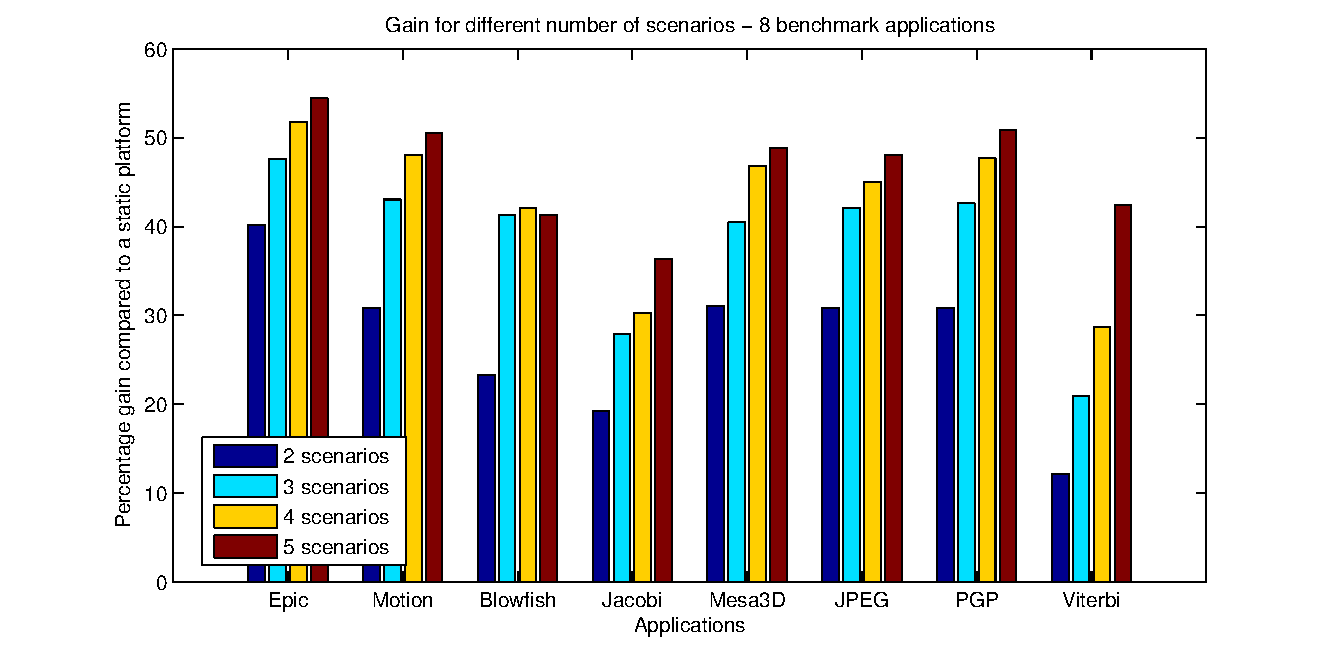
\includegraphics[width=1.1\textwidth]{C/6appsGains.pdf}
\caption{Energy gain for increasing number of system scenarios - Static platform corresponds to 0\%}
\label{fig:gainsC}
\end{figure}

\begin{figure}
\centering
\includegraphics[width=0.75\textwidth]{C/banks2.pdf}
\caption{Bank sizes for the most efficient of the tested organizations for each benchmark}
\label{fig:banksC}
\end{figure}

\subsection{Classification of the Applications}

The introduction of a second system scenario results in energy gains between 15\% and  40\%  for the tested applications. 
Depending on the application's dynamism the maximum reported energy gains range from around 35\% to 55\%. 
As expected according to the categorisation presented in subsection~\ref{sec:categorisationC}, higher energy gains are achieved for applications with more dynamic memory requirements, i.e., bigger difference between the minimum and maximum allocated size. 
The maximum gains for JPEG, motion estimator, mesa 3D and PGP are around 50\% while blowfish, jacobi, and Viterbi decoders are around 40\%.

\begin{center}
	\begin{table}
	\caption{Range of energy gains on the memory subsystem}
	\label{tab:ranges}
	{
	\begin{tabular}{|c|c|c|c|c|c|c|c|}
		\hline
		\multicolumn{2}{|c|}{\textbf{EPIC}} &
		\multicolumn{2}{c|}{\textbf{Motion}} &
		\multicolumn{2}{c|}{\textbf{Blowfish}} &
		\multicolumn{2}{c|}{\textbf{Jacobi}}
		\\ 
		\cline{1-8}
		Min & Max & Min & Max & Min & Max & 
		Min & Max \\ 
		\hline 
		40.6\% & 55.1\% & 31.2\% & 50.1\% & 23.5\% & 42.0\% & 
		19.8\% & 35.9\% \\ 
		\hline 

		\multicolumn{2}{|c|}{\textbf{Mesa3D}} &
		\multicolumn{2}{c|}{\textbf{JPEG}} &
		\multicolumn{2}{c|}{\textbf{PGP}} &
		\multicolumn{2}{c|}{\textbf{Viterbi}} \\ 
		\cline{1-8}
		Min & Max & Min & Max & Min & Max & 
		Min & Max \\ 
		\hline 
		31.3\% & 49.2\% & 31.1\% & 48.9\% & 
		30.6\% & 51.2\% & 12.5\% & 42.4\% \\ 
		\hline
		
	\end{tabular}}
	\end{table}
\end{center}

As the number of system scenarios that are implemented on the memory subsystem increases, the energy gains improve since variations in memory requirements can be better exploited with more configurations. 
However, the improvement with increasing numbers of system scenarios differ depending on the kind of dynamism present in each application. 
The application with the highest variation in distribution of memory requirements is the Viterbi encoder/decoder and gains around 10\% is seen for every new memory bank added, even for a platform growing from four to five banks. 
In contrast, the application with the lowest number of different cases, blowfish, cannot further exploit a platform with more than three banks. 
Another case in which smaller energy gains are achieved, after a certain number of platform supported system scenarios have been reached, is the PGP encryption algorithm. 
In this benchmark the introduction of more scenarios has an energy impact of less than 5\% after the limit of three system scenarios has been reached. 

\subsection{Switching Overhead}

The switching cost increases for an increasing number of system scenarios due to the increasing frequency of platform reconfiguration. 
This overhead reduces the achieved gain, but for up to 5 scenarios we still see improvements for all but one of our benchmarks. 
The switching cost is below 2\% even for a platform with 5 memory banks in all cases.
Apart from the number of scenarios, the switching cost depends on the sensitivity of the variable used for scenario identification. 
A change of value on the identification variable indicates potentially a new scenario. 
For an increasing frequency of changes, the switching cost increases.

\subsection{Comparison with Use Case Scenario}

Comparative results from applying a use case scenario approach as a reference are presented in Fig.~\ref{fig:usecaseC}. 
Reported energy gains for both use case scenarios and the most efficient case of the system scenarios are given assuming a static platform as a base (0\%). 
Use case scenarios are generated based on a higher abstraction level that is visible as a user's behavior. 
For example, use case scenarios for image processing applications generate three scenarios, if large, medium and small are the image sizes identified by the user. 
Similarly, use case scenarios for JPEG compression identify only low and high compression as options and motion estimation is performed on I, P and B video frames, without exploring fine grain differences inside a frame. 
In general, use case scenario identification can be seen as more coarse compared to identification on the detailed system implementation level. 
As seen in Fig.~\ref{fig:usecaseC} the use case gains are superior only to a static platform.

\begin{figure}
\centering
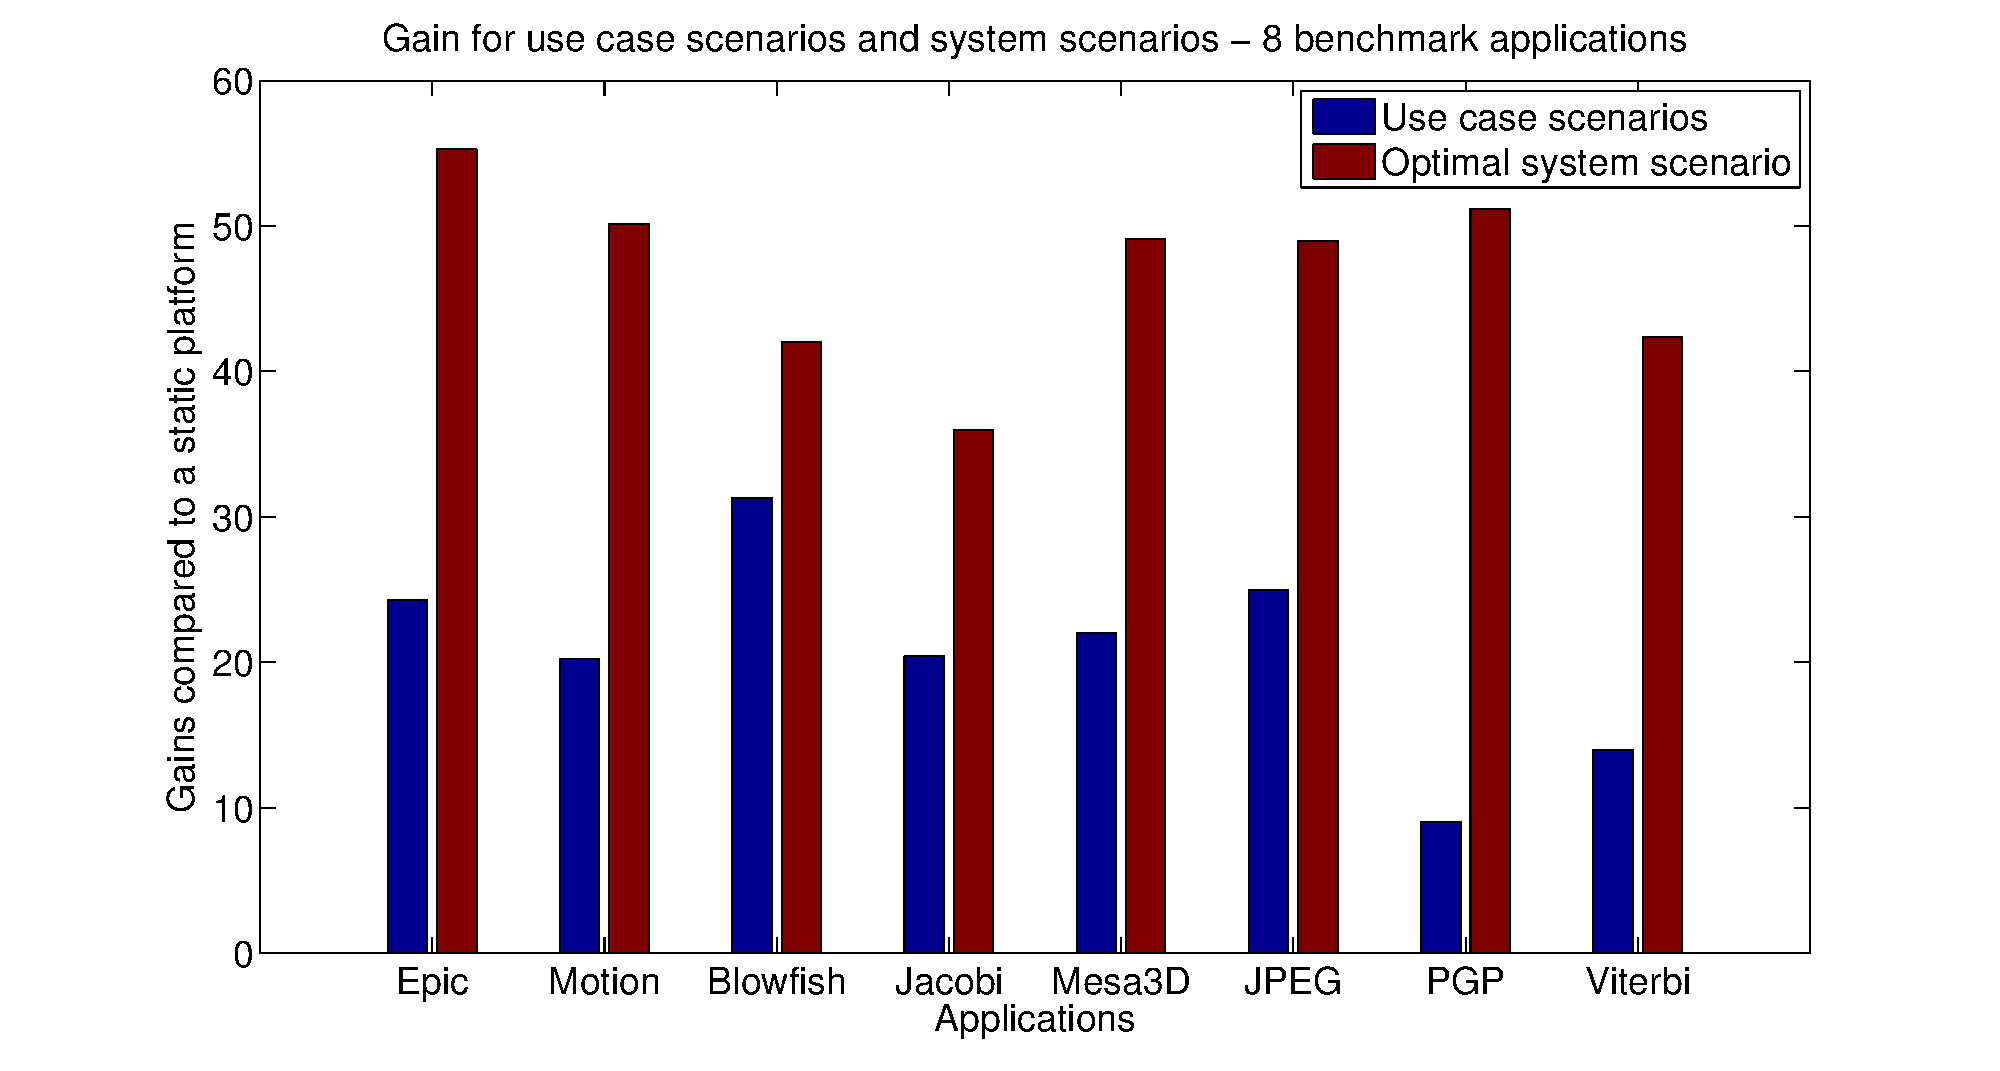
\includegraphics[width=\textwidth]{C/usecase.pdf}
\caption{Energy gain for use case scenarios and system scenarios}
\label{fig:usecaseC}
\end{figure}

\subsection{Run-Time Overhead}  

The reported energy gains are for the memory subsystem. 
As motivated in Section~\ref{sec:motivationC} this has previously been shown to be a major contributor to the total energy consumption. 
An additional energy overhead from the system scenario approach can be found in the processor performing the run-time system scenario detection and switching. 
This overhead is partly incorporated in $E_{SleepActive}$, in particular if traditional system scenarios are already implemented so that the only overhead is the addition of memory-awareness.
The run-time overhead is kept low, because the run-time manager is active for less than 1\% of the time needed for the execution of the application. 

\section{Conclusions}
\label{sec:conclusionC}

The scope of this work is to apply the memory-aware system scenario methodology to a wide range of multimedia application and test its effectiveness based on an extensive memory energy model. 
A wide range of applications is studied that allow us to draw conclusions about different kinds of dynamic behavior and their effect on the energy gains achieved using the methodology. 
The results demonstrate the effectiveness of the methodology reducing the memory energy consumption with between 35\% and 55\%. 
Since memory size requirements are still met in all situations, performance is not reduced. 
The memory-aware system scenario methodology is suited for applications that experience dynamic behavior with respect to memory organization utilization during their execution.

\addcontentsline{toc}{section}{Bibliography}	
\bibliographystyle{plain}
\bibliography{reference}
%\begin{thebibliography}{42}
%\providecommand{\natexlab}[1]{#1}
%\providecommand{\url}[1]{{#1}}
%\providecommand{\urlprefix}{URL }
%\expandafter\ifx\csname urlstyle\endcsname\relax
%  \providecommand{\doi}[1]{DOI~\discretionary{}{}{}#1}\else
%  \providecommand{\doi}{DOI~\discretionary{}{}{}\begingroup
%  \urlstyle{rm}\Url}\fi
%\providecommand{\eprint}[2][]{\url{#2}}
%
%\bibitem{Ben00b}
%Benini L, Macii A, Poncino M (2000) A recursive algorithm for
%  low-power memory partitioning. In: Proceedings of the 2000 intr symp on Low
%  Power Electronics and Design, pp 78 -- 83
%
%\bibitem{Ben00c}
%Benini L, et~al (2000) Increasing energy efficiency of embedded
%  systems by application-specific memory hierarchy generation. Design Test of
%  Computers, IEEE 17(2):74 --85, \doi{10.1109/54.844336}
%
%\bibitem{Gem5}
%Binkert N, et~al (2011) The gem5 simulator. SIGARCH Comput Archit News
%  39(2):1--7
%
%\bibitem{Che09}
%Cheung E, et~al (2009) Memory subsystem simulation in software tlm/t models.
%  In: Proceedings of Asia and South Pacific Design Automation Conference,
%  2009., pp 811 --816, \doi{10.1109/ASPDAC.2009.4796580}
%
%\bibitem{Chu02}
%Chung EY, et~al (2002) Contents provider-assisted dynamic voltage scaling for
%  low energy multimedia applications. In: Proceedings of the 2002 intr symp on
%  Low Power Electronics and Design, ISLPED '02, pp 42--47
%
%\bibitem{Fil12}
%Filippopoulos I, et~al (2012) Memory-aware system scenario approach energy
%  impact. In: NORCHIP, 2012, pp 1 --6, \doi{10.1109/NORCHP.2012.6403111}
%
%\bibitem{Garcia}
%Garcia P, et~al (2006) An overview of reconfigurable hardware in embedded
%  systems. EURASIP J Embedded Syst 2006(1):13--13
%
%\bibitem{Gheorghita2007}
%Gheorghita SV, et~al (2009) System-scenario-based design of dynamic embedded
%  systems. ACM Trans Des Autom Electron Syst 14(1):3:1--3:45
%
%\bibitem{Gonzalez1996}
%Gonzalez R, Horowitz M (1996) Energy dissipation in general purpose
%  microprocessors. Solid-State Circuits, IEEE Journal of 31(9):1277 --1284,
%  \doi{10.1109/4.535411}
%
%\bibitem{mibench}
%Guthaus M, Ringenberg J, Ernst D, Austin T, Mudge T, Brown R (2001) Mibench: A
%  free, commercially representative embedded benchmark suite. In: Workload
%  Characterization, 2001. WWC-4. 2001 IEEE Int. Workshop on, IEEE, pp 3--14
%
%\bibitem{Elena2010}
%Hammari E, Catthoor F, Kjeldsberg PG, Huisken J, (2010) Application of medium-grain multiprocessor mapping
%  methodology to epileptic seizure predictor. In: NORCHIP, 2010, pp 1 --6,
%  \doi{10.1109/NORCHIP.2010.5669489}
%  
%\bibitem{Elena2012}
%Hammari E, Catthoor F, Kjeldsberg PG, Huisken J, Tsakalis K, Iasemidis L, (2012) Realization of dynamical electronic systems. In: The International Conference on Engineering of Reconfigurable Systems and Algorithms, 2012 
%
%\bibitem{graybox}
%Himpe S, et~al (2002) {M}{T}{G}* and grey-box: modeling dynamic multimedia
%  applications with concurrency and non-determinism. In: System Specification
%  and Design Languages: Best of FDL02
%
%\bibitem{Hul11}
%Hulzink J, et~al (2011) An ultra low energy biomedical signal processing system
%  operating at near-threshold. IEEE Trans on Biomedical Circuits and Systems
%  5(6):546--554
%  
%\bibitem{Math}
%Ryser HJ (1963). Combinatorial mathematics. New York.
%
%\bibitem{Ang13b}
%Kritikakou A, et~al (2013) Near-optimal \& scalable intra-signal in-place for non-overlapping \& irregular access scheme. ACM Trans Design Automation of Electronic Systems (TODAES) ACM, New York, NY, USA.
%
%\bibitem{Ang13}
%Kritikakou A, et~al (2013) A scalable and near-optimal representation for storage size management. ACM Trans Architecture and Code Optimization. (accepted)
%
%\bibitem{mediabench}
%Lee C, et~al (1997) Mediabench: a tool for evaluating and synthesizing
%  multimedia and communicatons systems. In: Proceedings of the 30th annual
%  ACM/IEEE international symposium on Microarchitecture, IEEE Computer Society,
%  pp 330--335
%
%\bibitem{tcm}
%Ma Z, et~al (2007) Systematic Methodology for Real-Time Cost-Effective Mapping
%  of Dynamic Concurrent Task-Based Systems on Heterogenous Platforms, 1st edn.
%  Springer Publishing Company, Incorporated
%
%\bibitem{Mac02}
%Macii A, Benini L, Poncino M (2002) Memory Design Techniques for Low-Energy
%  Embedded Systems. Kluwer Academic Publishers
%
%\bibitem{Mar03}
%Marchal P, et~al (2003) {S}{D}{R}{A}{M} energy-aware memory allocation for
%  dynamic multi-media applications on multi-processor platforms. In: DATE, pp 516--521
%
%\bibitem{Mei10}
%Meinerzhagen P, Roth C, Burg A (2010) Towards generic low-power area-efficient
%  standard cell based memory architectures. In: Circuits and Systems (MWSCAS),
%  2010 53rd IEEE Int. Midwest Symposium on, IEEE, pp 129--132
%
%\bibitem{Mei11}
%Meinerzhagen P, et~al (2011) Benchmarking of standard-cell based memories in
%  the sub-vt domain in 65-nm cmos technology. IEEE Transactions on Emerging and
%  Selected Topics in Circuits and Systems 1(2)
%
%\bibitem{narasinga}
%Miniskar NR (2012) System scenario based resource management of processing
%  elements on mpsoc. PhD thesis, Katholieke Universiteit Leuven
%
%\bibitem{Pal06}
%Palkovic M, Catthoor F, Corporaal H (2006) Dealing with variable
%  trip count loops in system level exploration. In: Proceedings of the 4th Workshop
%  on Optimizations for DSP and Embedded Systems, IEEE and ACM SIGMICRO, pp
%  21--30
%
%\bibitem{Pal07}
%Palkovic M, Corporaal H, Catthoor F (2007) Heuristics for scenario creation to
%  enable general loop transformations. In: System-on-Chip, 2007 Int. Symposium
%  on, pp 1 --4
%\bibitem{Pal06b}
%Palkovic M, et~al (2006) Systematic preprocessing of data
%  dependent constructs for embedded systems. Journal of Low Power Electronics,
%  Volume 2, Number 1
%
%\bibitem{Pgk01}
%Panda PR, et~al (2001) Data and memory optimization techniques for embedded
%  systems. ACM Trans Des Autom Electron Syst 6(2):149--206
%
%\bibitem{Poly}
%Pouchet L (2012) Polybench: The polyhedral benchmark suite
%
%\bibitem{Ben99}
%Simunic T, et~al (1999) Cycle-accurate simulation of energy consumption in
%  embedded systems. In: Proceedings of the 36th Design Automation Conference,
%  1999., pp 867--872
%  
%\bibitem{abraham1999automatic}
%Abraham SG, Mahlke SA (1999) Automatic and efficient evaluation of memory
%  hierarchies for embedded systems. In: Proceedings of the Microarchitecture, 1999. MICRO-32.
%  . 32nd Annual International Symposium on, IEEE, pp 114--125
%
%\bibitem{chen1999loop}
%Chen F, Sha EHM (1999) Loop scheduling and partitions for hiding memory
%  latencies. In: Proceedings of the 12th international symposium on System
%  synthesis, IEEE Computer Society, p~64
%
%\bibitem{chen2000synthesis}
%Chen S, Postula A (2000) Synthesis of custom interleaved memory systems. Very
%  Large Scale Integration (VLSI) Systems, IEEE Transactions on 8(1):74--83
%
%\bibitem{grun2000mist}
%Grun P, Dutt N, Nicolau A (2000) Mist: An algorithm for memory miss traffic
%  management. In: Proceedings of the 2000 IEEE/ACM international conference on
%  Computer-aided design, IEEE Press, pp 431--438
%
%\bibitem{jacob1996analytical}
%Jacob BL, Chen PM, Silverman SR, Mudge TN (1996) An analytical model for
%  designing memory hierarchies. Computers, IEEE Transactions on
%  45(10):1180--1194
%
%\bibitem{jantsch1994hardware}
%Jantsch A, Ellervee P, Hemani A, {\"O}berg J, Tenhunen H (1994)
%  Hardware/software partitioning and minimizing memory interface traffic. In:
%  Proceedings of the conference on European design automation, IEEE Computer
%  Society Press, pp 226--231
%
%\bibitem{kandemir2001improving}
%Kandemir M, Sezer U, Delaluz V (2001) Improving memory energy using access
%  pattern classification. In: Proceedings of the 2001 IEEE/ACM international
%  conference on Computer-aided design, IEEE Press, pp 201--206
%
%\bibitem{li1999hardware}
%Li Y, Wolf WH (1999) Hardware/software co-synthesis with memory hierarchies.
%  In: Computer-Aided Design of Integrated Circuits and Systems, IEEE Transactions
%  on 18(10):1405--1417
%
%\bibitem{oshima1997high}
%Oshima Y, Sheu BJ, Jen SH (1997) High-speed memory architectures for multimedia
%  applications. Circuits and Devices Magazine, IEEE 13(1):8--13
%
%\bibitem{passes1995multi}
%Passes N, Sha EM, Chao LF (1995) Multi-dimensional interleaving for
%  time-and-memory design optimization. In: Proceedings of the Computer Design: VLSI in Computers
%  and Processors, 1995. ICCD'95, 1995 IEEE International
%  Conference on, IEEE, pp 440--445
%
%\bibitem{schmit1997synthesis}
%Schmit H, Thomas DE (1997) Synthesis of application-specific memory designs.
%  Very Large Scale Integration (VLSI) Systems, IEEE Transactions on
%  5(1):101--111
% 
%\bibitem{usecase}
%Gutierrez JJ, et~al (2008). A case study for generating test cases from use cases. In: Research Challenges in Information Science, 2008. RCIS 2008. Second International Conference on (pp. 209-214). IEEE.
%
%\end{thebibliography}
%
%
%\end{document}

\chapter{Integrated Exploration Methodology for Data Interleaving and Data-to-Memory Mapping on SIMD architectures}
\label{interleaving}

\begin{center}
Iason Filippopoulos, Namita Sharma, Francky Catthoor, \\ Per Gunnar Kjeldsberg and Preeti Ranjan Panda
\\
ACM Transactions on Embedded Computing Systems
\\
Submitted in 2015 
\\
(currently under second round of review)
\end{center}
\afterpage{\null\newpage}
\newpage

\vspace*{\fill}
\phantomsection
\section*{\hspace*{\fill} Abstract \hspace*{\fill}}
\addcontentsline{toc}{section}{Abstract}
This work presents a methodology for efficient exploration of data interleaving and data-to-memory mapping options for SIMD (Single Instruction Multiple Data) platform architectures.
The system architecture consists of  a reconfigurable clustered scratch-pad memory and a SIMD functional unit, which performs the same operation on multiple input data in parallel. 
The memory accesses contribute substantially to the overall energy consumption of an embedded system executing a data intensive task. 
The scope of this work is the reduction of the overall energy consumption by increasing the utilization of the functional units and decreasing the number of memory accesses.
The presented methodology is tested using a number of benchmark applications with irregularities in their access scheme.
Potential gains are calculated based on the energy models both for the processing and the memory part of the system.
The reduction in energy consumption after efficient interleaving and mapping of data is between 40\% and 80\% for the complete system and the studied benchmarks.
\vspace*{\fill}
\afterpage{\null\newpage}
\newpage

\section{Introduction}

Energy is an important limiting factor for modern embedded systems.
New novel hardware solutions have been proposed to reduce the energy consumption.
On the processing side, SIMD architectures offer new possibilities for potential improvements on the performance and the energy consumption.
On the memory side, modern memory architectures provide different energy modes and clustered scratch-pad memory banks that can operate independently, offering more options for reducing energy consumption.
Dynamic and data intensive algorithms are implemented on embedded systems.
Data intensive applications have often holes in their memory accesses, meaning that the data in memory are not always accessed in order.
The lack of spatial locality and the presence of redundant data results in lower utilization of the hardware resources, given that a conventional approach is employed for the handling of data.
This problem motivates the development of a methodology to improve the management of the data.

In order to tackle this problem we propose an interleaving exploration that aims to increase spatial locality and reduce the memory accesses on redundant data.
The goal of this work is to improve the energy consumption for data intensive applications without any loss on the application's performance. 
We focus on single instruction multiple data (SIMD) architectures and explore applications that have irregularities in their access scheme. 
SIMD architectures can potentially increase the performance of an application, providing that the utilization of them is high. 
However, applications with irregular access patterns do not provide compact sequences of data that are suitable for high utilization. 
Hence the performance is lower than expected and the number of memory accesses is high due to the accessing of redundant data. 
In order to reduce the number of memory accesses and achieve higher utilization of the system architecture a systematic exploration of the interleaving options and memory mapping for an application's data is needed. 

A large number of papers have demonstrated the importance of the memory organization to the overall system energy consumption. 
As shown in \cite{Gonzalez1996} memory contributes around 40\% to the overall power consumption in general purpose systems. 
Especially for embedded systems, the memory subsystem accounts for up to 50\% of the overall energy consumption \cite{Che09} and the cycle-accurate simulator presented in \cite{Ben99} estimates that the energy expenditures in the memory subsystem range from 35\% up to 65\% for different architectures. 
The breakdown of power consumption for a recently implemented embedded system presented in \cite{Hul11} shows that the memory subsystem consumes more than 40\% of the leakage power on the platform. 
According to \cite{tcm}, conventional allocation and assignment of data done by regular compilers is suboptimal. 
Performance loss is caused by stalls for fetching data and data conflicts for different tasks, due to the limited size of memory and the competition between tasks. 

The energy consumption can be divided into two parts, namely the processing and the memory subsystem consumption.  
The energy needed for processing depends mainly on the utilization of the FUs and any potential stalls, if the memory cannot provide data at the needed rate.
The interleaving exploration can increase the utilization of the processing subsystem and reduce time penalties for data loading.   
The energy consumption in the memory subsystem is affected by the number of memory accesses and the energy per access. 
Again, the memory architecture and the data-to-memory mapping decisions have great impact on both the number of accesses and the energy per access.

This article is organized as follows. 
Section~\ref{sec:motivationalD} motivates the study of developing a methodology for optimization of the data interleaving exploration and the data-to-memory mapping. 
Section~\ref{sec:relatedD} surveys related work on both the interleaving and memory mapping exploration.
Section~\ref{sec:methodologyD} presents the general work-flow and the sequence of the methodology steps.
In Section~\ref{sec:platformD} the target platform is described accompanied by a detailed description of the employed SIMD architecture and the memory models.
The set of benchmarks is analyzed in Section~\ref{sec:applicationsD} and  
results of applying the described exploration methodology to the targeted applications is also presented there. Finally, conclusions are drawn in Section~\ref{sec:conclusionD}. 

\section{Motivational Example}
\label{sec:motivationalD}
%
Many different techniques have been proposed already to deal with the memory accesses and the potential memory bottlenecks. 
Authors in \cite{malik2000low} propose a low power cache memory for embedded systems that can optimize memory accesses based on application's requirements.
The goal in \cite{guo2013data} is to effectively utilize the scratch-pad memory of an embedded system in order to improve the memory accesses.
A recent survey of the developed techniques for improving cache power efficiency is presented in \cite{mittal2014survey}.
Reconfigurable hardware for embedded systems, including the memory architecture, is a topic of active research. 
An extensive overview of current approaches is found in \cite{Garcia}. 
The current work is complementary to the existing ones and focuses on the areas that has not been explored in detail as discussed in \ref{sec:relatedD}.

The approach presented in this paper differentiates by exploring both the data transformations and data-to-memory assignment aspects in the presence of a platform with dynamically configurable memory blocks and bus widths. 
Moreover, many methods for source code transformations, and especially loop transformations, have been proposed in the memory management context. 
These methods are fully complementary to our focus on data-to-memory assignment and should be performed prior to our step.
The contribution of the proposed work is the presentation of a combined approach that investigates the interleaving and memory mapping options for a reconfigurable SIMD architecture.  

To illustrate the sub-optimal utilization of SIMD architectures using conventional allocation and assignment of data, the simple example of Alg.~\ref{alg:motivationD} is used.
In this example, we assume that the desired result is always the sum of 4 elements from arrays \textit{A, B, C and D}. 
The access pattern shows an irregularity, as a result of the iteration index.
For every group of four sequential array elements, there is only one used for the calculation of the result and the other three are skipped.
An intuitive interleaving optimization is the interleaving of the arrays \textit{A, B, C and D}, in order to generate sequences of elements that are all useful on the calculation of the \textit{result} variable. 
A full interleaving exploration could reveal several options to produce larger sequences of array elements that are needed during the execution of Alg.~\ref{alg:motivationD}.
For example, the interleaving within the combined array ($A\vert B\vert C\vert D$) can result in a sequence of 8 accessed elements.
The sequence of 8 elements is achieved by combining every forth line of the combined array, i.e. line 0 and line 4 are placed next to each other resulting in a sequence of 8 useful elements.

\begin{algorithm}
\caption{Motivational Example Algorithm}
\label{alg:motivationD}
\begin{algorithmic}[1]
\STATE $N \gets 100$ 
\FOR {$i = 0 \to N$}
\STATE $result(i) \gets A(i) + B(i) + C(i) + D(i) $
\STATE $i \gets i + 4$ 
\ENDFOR
 \end{algorithmic}
\end{algorithm}

The initial data representation for the arrays \textit{A, B, C and D} is shown in Fig.\ref{fig:motivation}(a). 
The array elements that are accessed during the execution of the motivational example are marked with colors, in contrast to the elements that are not accessed.
The array elements are drawn in 25 lines with 4 elements on each line only for a better visual representation.
At this point there is no mapping to the memory architecture and no constraint regarding the number of lines or their width in the memory design.
The interleaving of the arrays \textit{A, B, C and D} is shown in Fig.\ref{fig:motivation}(c). 
Each line of the new interleaved array contains one elements from the initials arrays.
For example, the first line consists of the elements \textit{A(0), B(0), C(0) and D(0)}. 
The result of the interleaving is the construction of blocks consisting of 4 colored elements followed by blocks with 12 redundant elements.

Let us now consider possible data-to-memory mappings for the initial and interleaved array elements.
We assume here that he memory architecture either consists of one single memory large enough to fit all four arrays or of four memory banks with a combined memory size large enough to fit the four arrays.
The conventional approach with the initial set of data maps each array after each other in the single memory or maps each array in a separate bank.
A possible data-to-memory mapping for the initial set of data using four banks is presented in Fig.~\ref{fig:motivation}(b). 
The data-to-memory mapping for the constructed interleaved array is presented in Fig.~\ref{fig:motivation}(d).
The array is split into four parts and stored in the four different banks using the same memory architecture.
Each of the lines of the interleaved array is stored in the bank corresponding to modulo 4 of the array line.
For example, line $x$ is stored in bank $x \bmod 4$.
As a result only one forth of array A can be found in the first bank in contrast to the non-interleaving case, in which the whole array A is mapped in the first bank.

\begin{figure}
\centering
	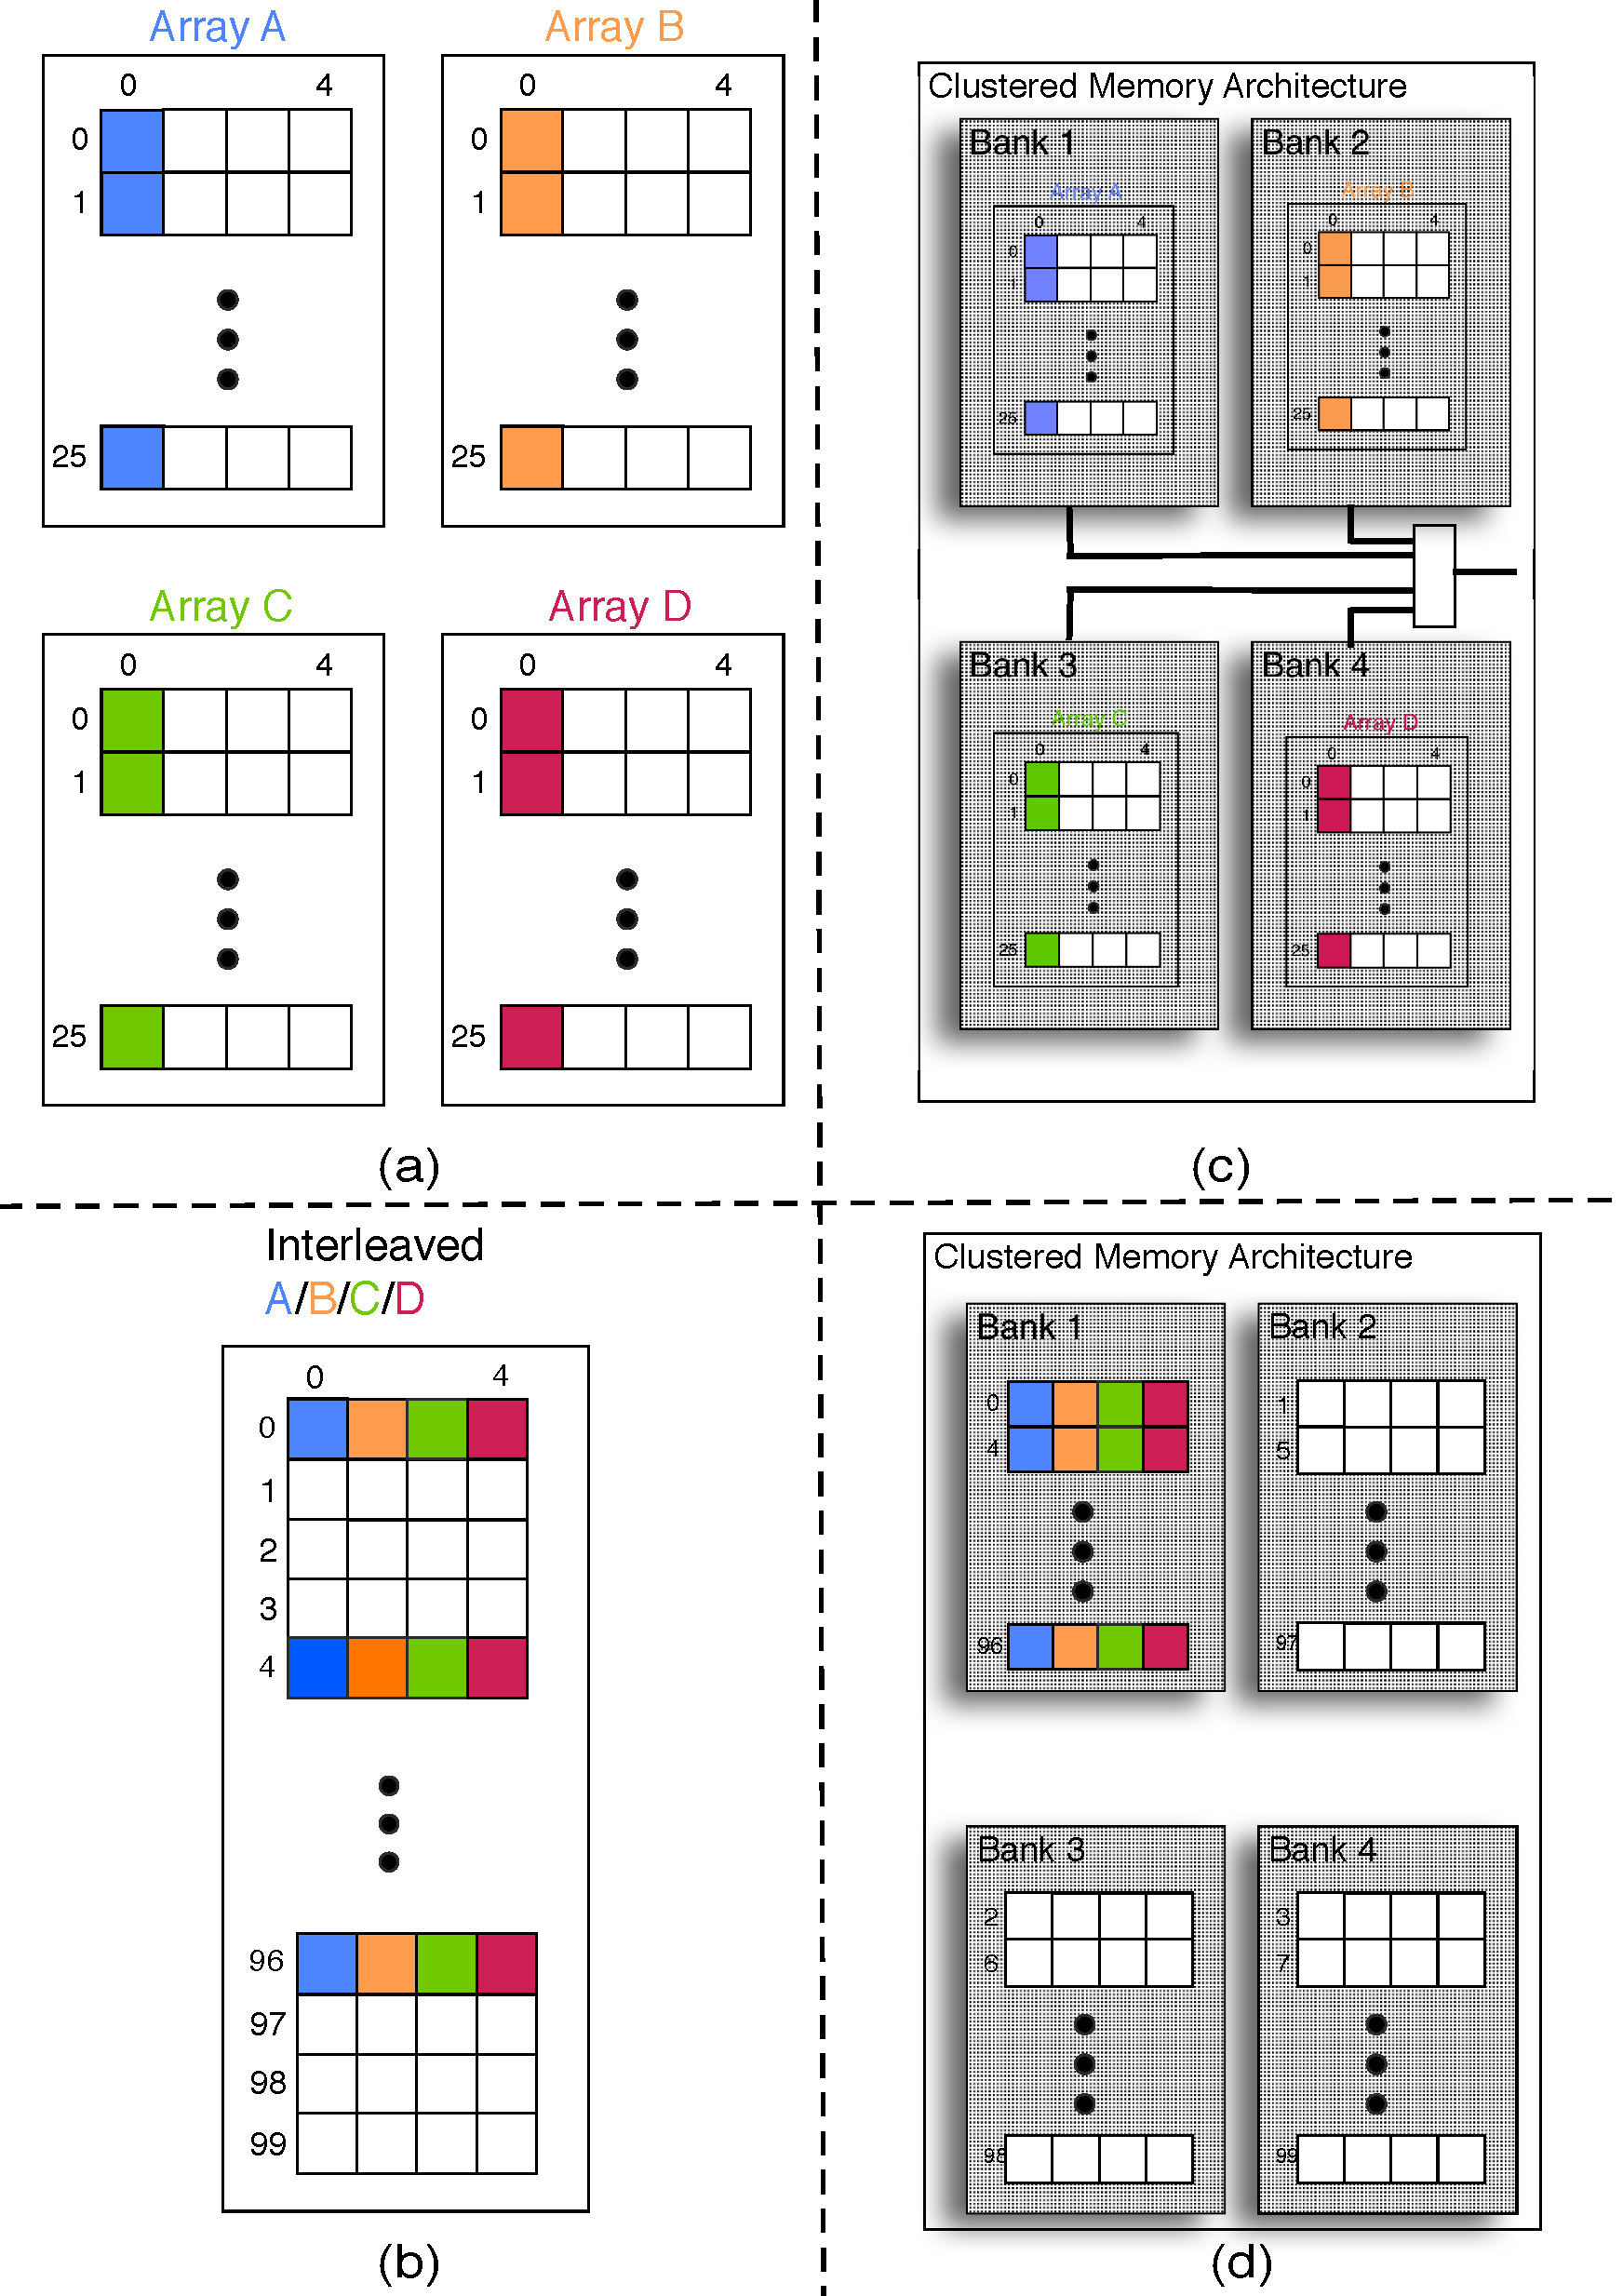
\includegraphics[width = 0.9\linewidth]{D/Images/motivation2.pdf}
	\caption{Motivational Example. Representation of the initial set of data (a) and the interleaved set of data (b). Data-to-memory mapping for the initial (c) and the interleaved data (d) on a clustered scratch-pad memory architecture.}	
	\label{fig:motivation}
\end{figure}

A quick estimation for the difference in the number of memory accesses between the two approaches presented in Fig.~\ref{fig:motivation} can be made.
The target architecture for the current work consists of a reconfigurable clustered memory architecture, a processing element that supports SIMD FUs and a wide bus between them.
The architecture is presented in detail in Sec. \ref{sec:platformD}.
The motivational example uses a system architecture with an SIMD ADD FU that performs operations over 4 array elements at a time and a memory to processor path that has a width of 4 elements. 
Each array element is assumed to have the size of one word.
The register file at the processor level can only store the iteration variable $i$ and 5 elements, which are the variables \textit{result, A, B, C and D}.
Without interleaving of data the number of memory accesses for each loop iteration is 4, because the elements \textit{A(i), B(i), C(i) and D(i)} are stored in different lines and different memory banks or one larger bank.
The overall number of memory accesses is:
	\begin{equation}
		\textit{25 loop iterations $\times$ 4 accesses per iterations = 100 memory accesses}.
	\end{equation}	 
After performing the data interleaving exploration there is only one memory access for each loop iteration, because the elements \textit{A(i), B(i), C(i) and D(i)} are stored in one memory line in the same bank.
The overall number of memory accesses is:
	\begin{equation}
		\textit{25 loop iterations $\times$ 1 accesses per iteration = 25 memory accesses}.
	\end{equation}	 	

A quick estimation for the difference in the energy consumption between the approaches presented in Fig.~\ref{fig:motivation} can be calculated using a simple energy model for the memory banks.
We assume that the energy cost of accessing a memory bank the size of one array is 1E, while the average leakage energy in the time needed for the execution of one loop iteration is 0.3E. 
The corresponding access and leakage numbers for a four times larger memory that can fit all the data together is  3E and 1.2E, respectively. 
The numbers reflects the fact that as a first order approximation access energy increases sub-linearly with increased memory size, while leakage increases linearly with memory size. 
The energy consumption for a large memory with non-interleaved data is:
	\begin{equation}
		\textit{100 $\times$ 3E + 100$\times$ 1.2E = 420E}.
	\end{equation}	
In this case there is a performance loss and an increased leakage energy, because all the accesses has to be done sequentially on the same memory.	
The energy consumption for a four bank memory architecture with non-interleaved data is:
	\begin{equation}
		\textit{100 $\times$ 1E + 4$\times$ 100$\times$ 0.3E = 220E}.
	\end{equation}	
The energy consumption for a large memory with interleaved data is:
	\begin{equation}
		\textit{25 $\times$ 3E + 25$\times$ 1.2E = 105E}.
	\end{equation}	
Finally, the energy consumption for a four bank memory architecture with interleaved data is:
	\begin{equation}
		\textit{25 $\times$ 1E + 1$\times$ 25$\times$ 0.3E = 32.5E}.
	\end{equation}			
It should be noted that the leakage energy in the last case is considered only for the one bank that is always accesses.
The memory banks that store redundant data are assumed switched to retention mode to minimize leakage.
The simple estimations presented in equations (1)-(6) shows that a pure interleaving optimization results in a 75\% reduction in the number of accesses.
A memory optimization based on an energy efficient four bank clustered memory architecture can also give an important energy reduction.
The energy gains are even greater when interleaved data are mapped to an efficient memory architecture.
The observations for this simple example motivates the further exploration of the data interleaving and the data-to-memory mapping for applications with irregularities in their accesses. 
%The performance is also higher as there are 75\% less memory accesses.
%The energy consumption due to memory leakage is also lower, as the access time for the memory and the execution time of the algorithm are shorter.

\section{Related work}
\label{sec:relatedD}

Many studies have been published in the area of data layout transformations and memory management. 
This work differentiates by presenting an integrated approach that combines the two areas. 
The combination is performed in a systematic way and the final result is better than the sum of the two individual optimizations.
The data transformations on the application level are studied in combination with the data-to-memory mapping on the hardware level.
An overview of the related work on those two areas is presented.

Data layout optimizations aim to arrange data in memory with the objective of improving system performance and energy through means such as reduced memory access count or reduced cache misses. 
Several generic data layout techniques have been explored by researchers at various levels in the memory hierarchy. 
In \cite{4},  cache partitioning, a layout technique for arrays, maps each array to different cache partitions to reduce conflicts. 
In \cite{5} authors address the problem for cache miss reduction by evaluating the tiling size for arrays and merging the arrays appropriately for each loop nest. 
Memory Hierarchy Layer Assignment (MHLA), an optimization methodology for data memory hierarchy presented in \cite{6}, determines for each data set an appropriate layer in the hierarchy and type of memory (single/dual port) taking data re-use into account. 
The strategy in \cite{7} partitions the variables to scratch-pad memory and DRAM to minimize interference between variables. 
 The cache-oriented techniques proposed earlier by researchers in \cite{8} do not find a straightforward application in our context, where the target system hardware consists of a scratch-pad memory and a SIMD functional unit.
 The current work explores the assignment of data to the memory and the effect of different interleaving decisions on the overall energy consumption.

Several techniques for designing energy efficient memory architectures for embedded systems are presented in \cite{Mac02}. 
The current work differentiates by employing a platform that is reconfigurable at run-time. 
In \cite{Pgk01} a large number of data and memory optimisation techniques, that could be dependent or independent of a target platform, are discussed. 
Again, reconfigurable platforms are not considered. 
The authors in \cite{Ben00b} present a methodology to generate a static application-specific memory hierarchy. 
Later, they extend their work in \cite{Ben00c} to a reconfigurable platform with multiple memory banks. 

In \cite{dymaxion} the authors tackle the problem of sub-optimal data structure layouts in GPUs with a large number of parallel cores, especially for programs that are designed with a CPU memory interface in mind. 
An API is presented, that allows programmers to improve CUDA programs by optimizing memory mappings in order to increase the efficiency of memory accesses. 
The main differences of the current work are the platform and the types of code transformations. 
We focus on an SIMD CPU and a dynamic clustered scratchpad memory compared to multicore GPUs and a static memory. 
We differentiate by focusing on interleaving as the preferred code transformation, being suitable for the target applications.
Another work that discusses memory layout for GPUs is presented in \cite{DL}.
The authors focus on off-chip DRAM memory optimization using a number of data layout transformations. 
We differentiate by focusing on the memory closest to the CPU. We also study data interleaving while the main focus in \cite{DL} is the transformations that increase data parallelism, which is more important for their multicore GPU architecture.
In \cite{3D} a number of common data reorganization operations such as shuffle, pack/unpack, swap, transpose, and layout transformations are presented. 
The goal is to study the cost of applying these operations in the memory at run-time. The target memory is 3D-stacked DRAM and additional hardware is employed in order to efficiently perform the reorganization operations with a low overhead. 
Apart from the different type of platform, the current work differentiates in the type of data reorganizations and the mapping of the reorganized data to the scratchpad memory at compilation time. 

The authors in \cite{abraham1999automatic}, \cite{jacob1996analytical} and \cite{li1999hardware} present methodologies for designing memory hierarchies.
Design methods with main focus on the traffic and latencies in the memory architecture are presented in \cite{chen1999loop}, \cite{grun2000mist}, \cite{jantsch1994hardware} and \cite{passes1995multi}.
Improving memory energy efficiency based on a study of access patterns is discussed in \cite{kandemir2001improving}.
Application specific memory design is a research topic in \cite{schmit1997synthesis}, while memory design for multimedia applications is presented in \cite{oshima1997high}.
The current work differentiates by presenting both a reconfigurable platform and the necessary data interleaving to better exploit the platform.
The discussed related work is not designed to handle dynamic variations on memory requirements due to employment of a static memory platform. 
Thus, it is expected to provide poor results when applied to the dynamic applications targeted in the current work.

The current work combines and expands in a non-trivial way, the interleaving exploration presented in \cite{sharma2013data} and the data to memory mapping methodology presented in \cite{filippopoulos2013exploration}. 
In \cite{sharma2013data} a memory dominant application is chosen, which normally suffers from data memory organization bottlenecks while implemented on conventional architectures. 
A data interleaving approach is employed in order to improve memory energy by reducing memory accesses.
Significant reduction in data memory energy consumption can be achieved if array data are interleaved, with no performance overhead.
In \cite{filippopoulos2013exploration} a memory-aware system scenario methodology is presented.
The variations in memory needs during the lifetime of an application are studied in order to optimize energy usage.
Different system scenarios capture the application's different resource requirements that change dynamically at run-time.
Many possible memory platform configurations and data-to-memory assignments are studied as system scenario parameters, which lead to a large exploration space.


The contribution of the proposed work is the development of a combined approach that investigates the interleaving and memory mapping options for a reconfigurable SIMD architecture.  
The current work combines and expands in a non-trivial way, the interleaving exploration presented in \cite{sharma2013data} and the data to memory mapping methodology presented in \cite{filippopoulos2013exploration}. 
The current work is more than a simple application of the two approaches, one after the other.
Such an approach cannot always guarantee a viable solution.
The reason is that for each different interleaving solution, there are a number of constraints on the placement of the data into the memory due to hardware limitations.
If the constraints are not propagated into the data-to-memory mapping step, the final solution suffers from data conflicts.
Different interleaving solutions introduce different constraints. 
Therefore, there is a need to develop an integrated methodology to achieve the improvements of both the approaches.

\section{Target Architecture and Energy Models}
\label{sec:platformD}

Selection of target platform is an important aspect of the exploration.
The motivational example in the previous section shows that the available choices on the memory models have a great impact on the overall energy consumption.
 The key feature needed in the platform architecture is the ability to efficiently support different memory sizes that are suitable for different data structures.
A generic architecture is presented in Fig.\ref{fig:arch}.
The scratch-pad memory consists of up to four memory banks. 
For more complex architectures the interconnection cost should be considered and analyzed separately for accurate results. 
Although power gating can be applied to the bus when only a part of a longer bus is needed, an accurate model of the memory wrapper and interconnection must be developed, which is beyond the scope of the current work.
The SIMD vector FU is assumed to perform instructions on multiple data.

Improving temporal locality of data accesses in cache is indeed important. 
The proposed architecture uses scratch-pad memories, however, and no cache memory is included in the current study.
Software controlled allocation is a significant feature for the current methodology, as the allocation of data can be fully determined by the designer at design-time.
The basic principles of the methodology are still applicable for hardware controlled caches, but some modifications would be needed to deal with the automatic resolution of hits and misses.
Temporal locality and data reuse are taken into consideration during the interleaving exploration.

The methodology explores different interleaving and data to memory mapping options for the reconfigurable architecture.
The optimal sizes are found based on the sizes of the data after the interleaving exploration.
The memory banks can operate independently and have different sizes.
The explored data lengths for the vector FU and the connections are 4, 8 and 16 elements.
The exploration is based on the available system models and results in the final system architecture.
Thus, the accuracy of the models influence the decisions taken during the design phase.

\begin{figure}
\centering
	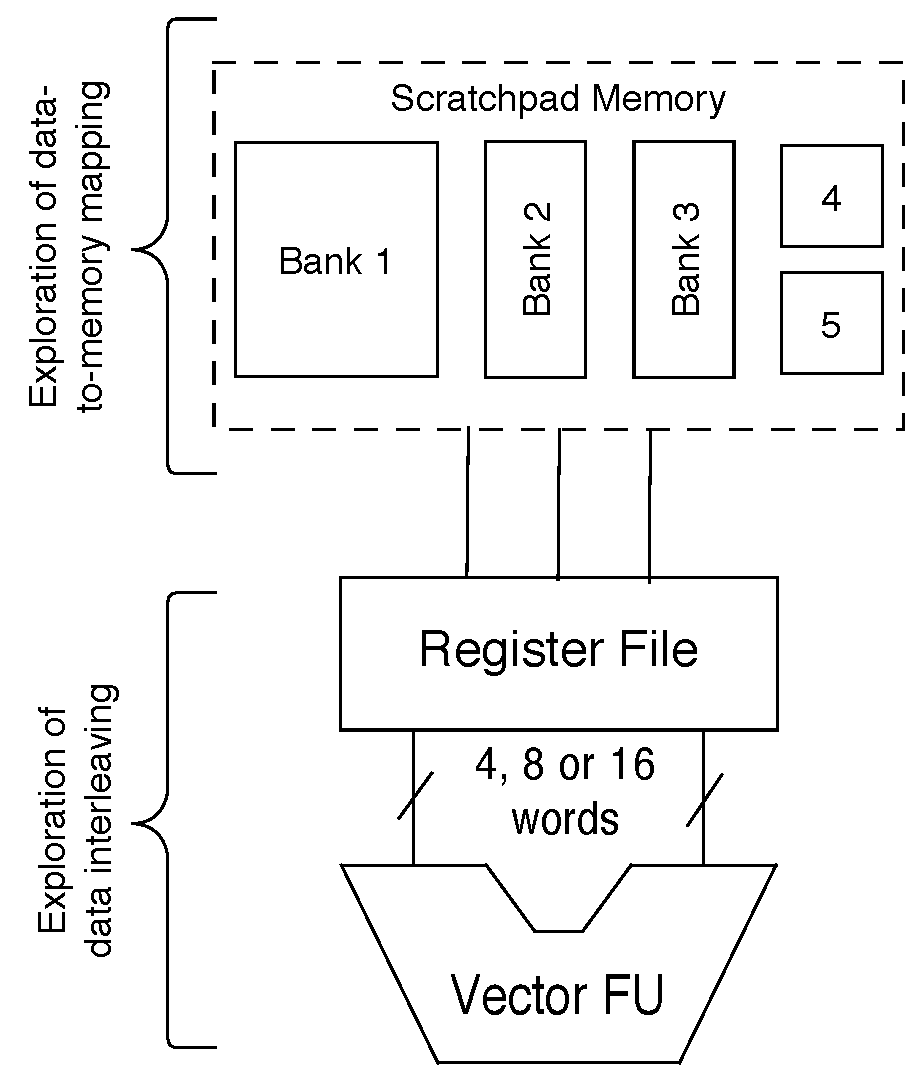
\includegraphics[scale = 0.5]{D/Images/Architecture.eps} 
	\caption{Exploration options and system knobs depending on a general platform architecture}
	\label{fig:arch}
\end{figure}

\subsection{Memory Models}

The dynamic memory organization is constructed using commercially available SRAM memory models (MM).
For those models delay and energy numbers are derived from a commercial memory compiler.
The commercial memory compiler is part of DesignWare Memory Compilers provided by Synopsys.
The logic libraries support a wide range of foundries and process technologies from 250nm to 28nm. 
The memories are optimized for low power, high performance and high density. A 40nm library was chosen for the current work.  
Of confidentiality reasons we are not allowed to reveal details of the compiler or process and the presented numbers are relative.
In addition, experimental standard cell-based memories (SCMEM) \cite{Mei11}  are  considered for smaller memories due to their energy and area efficiency for reasonably small storage capacities, as argued in \cite{Mei10}. 
The standard cell-based memories are synthesized using Cadence RTL compiler for TSMC 40nm standard library. 
Afterwards, power simulations on the synthesized design are carried out using Synopsys PrimeTime, in order to obtain energy numbers.
Both MMs and SCMEMs can operate under a wide range of supply voltages, thus support different operating modes that provide an important exploration space.
\begin{itemize}
\item Active mode: The normal operation mode, in which the memory can be accessed at the maximum supported speed. The supply voltage is 1.1V. 
The dynamic and leakage power are higher compared to the other modes.
Only in active mode the data are accessible without time penalties, in contrast to light and deep sleep modes.
In this work all the memory accesses are performed in active mode. 
\item Light sleep mode: The supply voltage in this mode is lower than active with values around 0.7V. 
The access time of the memory is significantly higher than the access time in active mode. 
Switching to active mode can be performed with a negligible energy penalty and a small time penalty of a few clock cycles (less than 10). 
Data is retained.  
\item Deep sleep mode: The supply voltage is set to the lowest possible value that can be used without loss of data. 
This voltage threshold is expected to be lower for SCMEMs than MM models and can be as low as 0.3V. 
The number of clock cycles needed for switching to active mode is higher compared to light sleep mode, typically in the range of 20 to 50 clock cycles depending on the clock speed. 
Consequently, the speed of the PE and the real-time constraints of the applications have to be taken into consideration when choosing light or deep sleep mode at a specific time.  
\item Shut down mode: Power-gating techniques are used to achieve near zero leakage power. 
Stored data is lost. 
The switch to active mode requires substantially more energy and time. 
However, switching unused memories to this mode, providing that their data are not needed in the future, results in substantial energy savings.
\end{itemize}  

The necessary energy and power information is available for the memory models. Relative values for a subset of them is presented in Table \ref{tab:models}. 
It is clearly shown that the choice of memory units has an important impact on the energy consumption.

\begin{table}
\centering
\caption{Relative dynamic energy for a range of memories with varying capacity and type\label{tab:models}}{
	\begin{tabular}{|c|c|c|c|c|c|}
		\hline
		\multirow{2}{*}{\textbf{Type}} & \textbf{Lines x} & \multicolumn{2}{c|}{\textbf{Dynamic Energy}} & \multicolumn{2}{c|}{Active from} \\ \cline{3-4}
		& \textbf{wordlength} & Read[nJ] & Write[nJ]  & Deep[uJ] & Light[uJ]\\ 
		\hline 
		MM & 32 x 8 &  $ 41.8 $ &  $ 32.4 $ & 0.223 &  0.031 \\ 
		\hline
		MM & 32 x 16 & $  67.9 $ &  $ 58.9 $ & 0.223 &  0.031\\ 
		\hline
		MM & 32 x 128 & $  433 $ &  $ 431 $ & 1.42 & 0.168\\ 
		\hline
		MM & 256 x 128 & $  448 $ &  $ 460 $ & 1.70 &  0.171\\ 
		\hline
		MM & 1024 x 128 & $  511 $ &  $ 575 $ & 2.81 & 0.179\\ 
		\hline
		MM & 4096 x 128 & $  960 $ &  $ 457 $ & 9.01 & 0.457\\ 
		\hline
		SCMEM & 128 x 128 & $  250 $ &  $ 8 $ & 1.51 &  0.045\\ 
		\hline
		SCMEM & 1024 x 8 & $  17  $ &  $ 6  $ & 0.325 &  0.021\\ 
		\hline
	\end{tabular}}
\end{table}

\subsection{Functional Unit Models}

The processing of the interleaved data is performed in the part of the architecture consisting of the SIMD FU and the central vector register file, as shown in Fig.\ref{fig:arch}.
 The bus between the memory part and the processing part is  256 bit wide.
 The wide bus allows testing for word length of 4, 8 and 16 elements, assuming that each array element is 16 bit wide.
 The different word lengths provide different design options for the vector FU.
This processor belongs to the class of coarse-grain reconfigurable array (CGRA) processors and is described in more detail in \cite{lee2003compilation}.
The HDL model of the processor is synthesized using Cadence RTL compiler \cite{cadencecompiler} and the energy numbers are extracted using Synopsys Primepower \cite{kai2003synopsys}.

For efficient utilization of the vector FU, the register file has a wide interface with the clustered scratch-pad memory. 
Since the target architecture is a configurable processor that can be customized in various ways, the standard evaluation and execution mechanism is to run the programs on a processor simulator. 
An XML based language is used to describe the architecture, and a cycle-accurate simulator of the processor is used to simulate the generated code on the architecture. The XML provides a structural way of describing the architecture presented in Fig. 2 including the different components, the parameters of each component, and the relationship between them. The XML description generates a graphical representation of the architecture and is the input for the simulator as presented in \cite{xml}. The chosen simulator is developed for coarse-grained reconfigurable architectures and is suitable in our case, because of the dynamic parameters of our architecture.
 
The energy consumption information for different types of instructions and different widths is available for the FU models.
The width of the FU corresponds to the number of pairs of array elements on which the specific instruction is performed.
Relative values for a subset of them is presented in Table \ref{tab:models2}. 
It is clearly shown that the wider FUs have a significantly higher energy consumption compared to FUs that operate on only two element.
Thus, it is important to achieve high utilization of wider FUs to achieve both performance and energy gains.

\begin{table}
\centering
\caption{Relative dynamic energy for different FU models\label{tab:models2}}{
	\begin{tabular}{|c|c|c|}
		\hline
		\textbf{Type of FU instruction} & \textbf{Width} & \textbf{Dynamic Energy [J]} \\ 
		\hline 
		ADD  & 1 & 5.70E-08 \\ 
		\hline
		ADD  & 4 & 2.28E-07 \\ 
		\hline
		MULT  & 1 & 2.48E-07 \\ 
		\hline
	 	MULT complex  & 1 & 5.33E-07 \\ 
		\hline
		MULT  & 4 & 1.03E-06 \\ 
		\hline
		MULT complex  & 4 & 1.95E-06 \\ 
		\hline
		\end{tabular}}	
\end{table}

\section{System Design Exploration Work-flow}
\label{sec:methodologyD}

\begin{figure}
\centering
	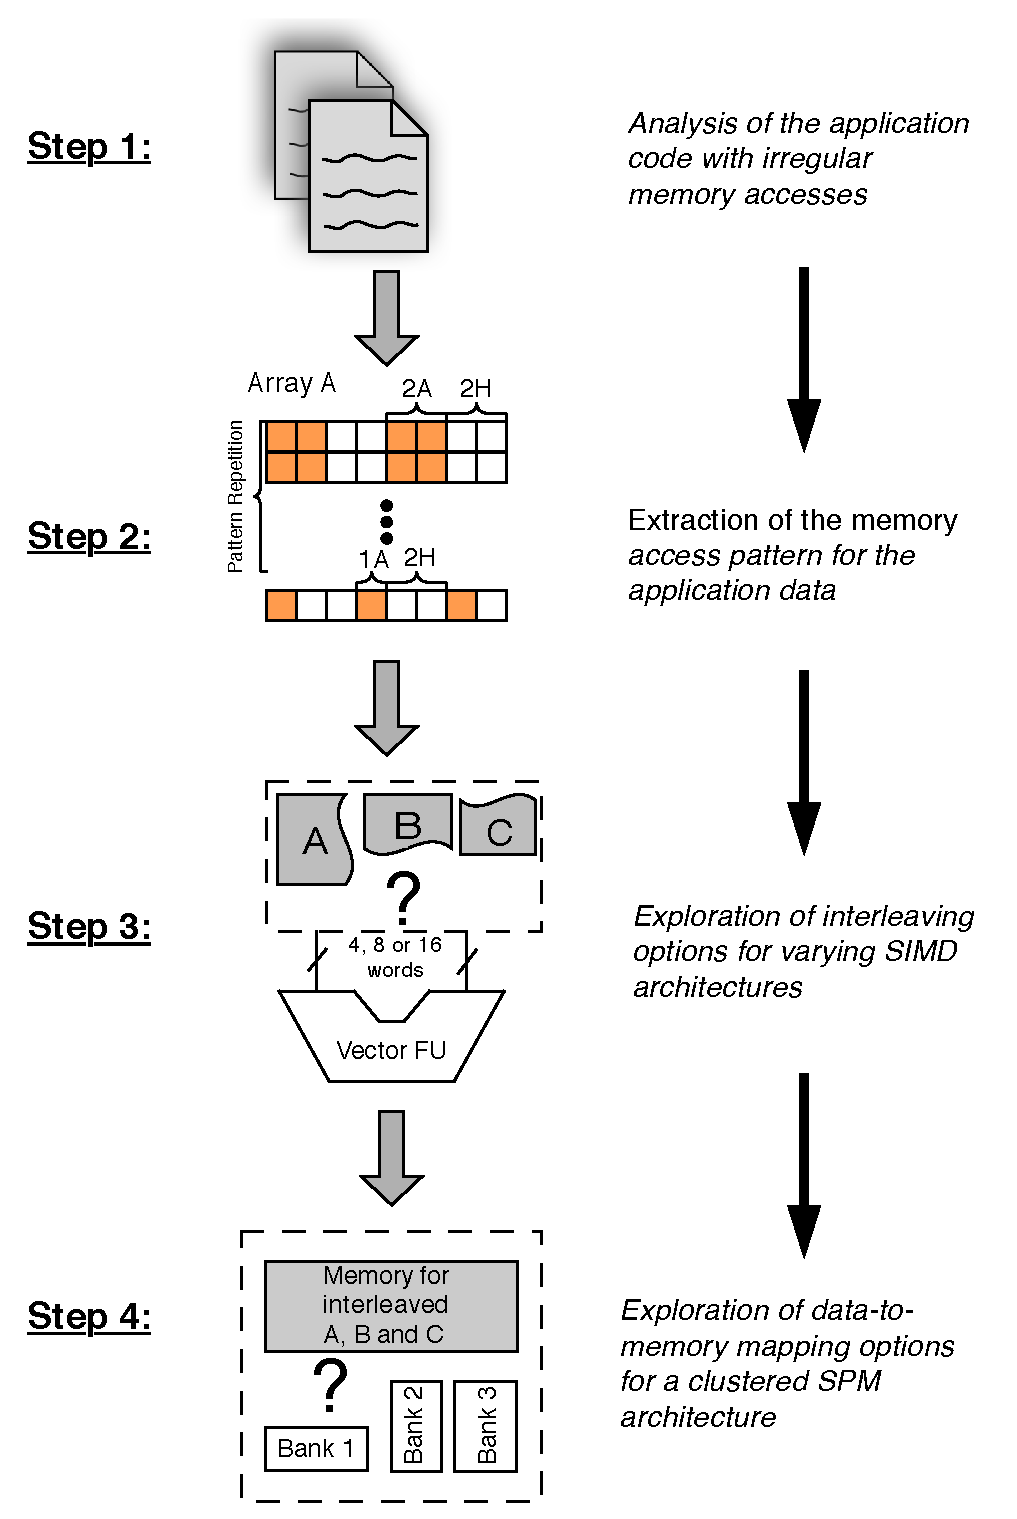
\includegraphics[scale = 0.6]{D/Images/workflow2.eps} 
	\caption{Methodology steps}
	\label{fig:workflow}
\end{figure}

As motivated in the previous sections a systematic exploration of the interleaving options and the data-to-memory mapping possibilities is necessary.
The input to the work-flow is the application code and the output of the exploration is an efficient solution for the interleaving of the data and a mapping to a reconfigurable system architecture based on the available models presented in Sec.\ref{sec:platformD}.
The exploration space consists of the potential combinations between the different arrays and the different scratch-pad memory architectures, which combine memories of different types and sizes.

The overall work-flow is presented in Fig.\ref{fig:workflow}. 
The first step of the methodology is the analysis of the application code. 
The methodology is applicable to any application.
However the applications that can benefit more from the proposed methodology are the ones with holes in their access patterns.
The second step is the extraction of the access pattern for each data structure present on the application code.
The third step is the interleaving exploration, which explores all the different options for the re-arrangement of the data.
The aim of this step is the construction of compact sets of data by using defined operations between the available access patterns.
The goal is to better utilize the different width of the vector FUs. 
The result of the interleaving is a set of data with a reduced number of holes.
The forth step is the mapping of the interleaved data set to the clustered memory architecture.

Some significant changes are needed in order to combine the different techniques in a functional work-flow.
The interleaving and the data-to-memory mapping exploration steps have to be modified and a simple concatenation is not sufficient.
The results of the interleaving exploration are given as constraints to the mapping exploration.
The constraints stir the exploration in a potentially different solution compared to the result of the data-to-memory mapping exploration without the interleaving constraints.
The interleaving exploration finds solutions for the different bus widths and then all the different solutions are propagated to the mapping exploration.
The mapping exploration takes all the interleaving constraints into consideration.
Thus, the data-to-memory mapping solutions using the constraints are in general different from the solutions provided in a conventional approach.
The propagation of the constraints is explained in more detail later. 

The application is fully analyzed at design-time, because of the time consuming nature of the task. 
The access patterns are extracted in software and the possible interleaving options are explored. 
The mapping to the specific target architecture is also fully decided at design-time.
The data-to-memory mapping exploration takes into consideration the platform and code limitation and proposes a mapping without data and bank conflicts.
The employment of a scratchpad memory architecture is crucial for this.
In contrast to cache memory systems, in which the mapping of data elements is done at run-time, in scratchpad memory systems the mapping is performed by the programmer or the compiler \cite{ishitobi2007code}. 
The address mapping follows the principles presented in \cite{address} and \cite{sharma2015array}. 
Unlike the cache memory, the scratchpad memory does not need tag search operations and it is the responsibility of the programmers or compilers to correctly allocate code and data on the scratchpad memory \cite{steinke2002assigning}.
This is possible for small embedded systems designed to run one or a limited set of specific applications. 
For other types of systems and applications, a cache memory can be the preferred solution as the detection of a cache hit or miss is done automatically and any conflicts can also be resolved by the platform at run-time.
In our case, the application and the memory system are fully analyzed and the allocation of data to a scratchpad memory can be easily done and offers an energy efficient solution.

\subsection{Formal Model Representation of Access Patterns }

A representation model for the memory access patterns is employed in order to formally present each step of the methodology.
The model presented in \cite{Ang13} is a generic model suitable for irregular iteration spaces on arrays.
The irregularities are created by the application code access statements in a conditional loop structure.

When an array element is accessed during the code execution, it is represented with an A(Access).
Otherwise, there is a hole in the access pattern represented with an H(Hole) as shown in Fig.\ref{fig:pattern}.
The sequence of accesses and holes is usually repeated periodically, because normally the loop conditions are not totally random.
Thus we can define the frequency of each access pattern.
The analysis of the application code results in the access patterns and their corresponding frequencies, which is the necessary input for the next step in the work-flow.

\begin{figure}
\centering
	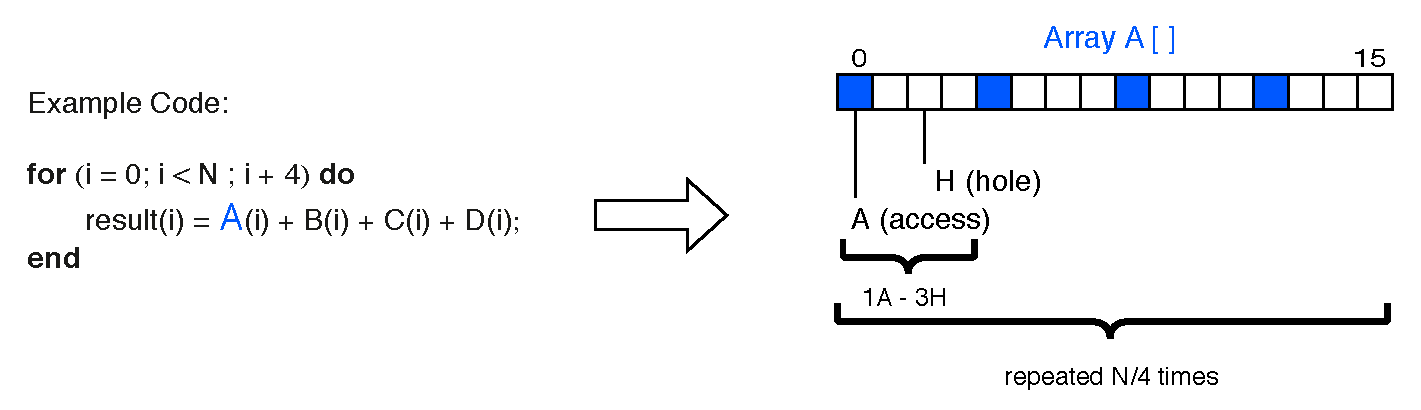
\includegraphics[width=\linewidth]{D/Images/AHpattern.eps} 
	\caption{Extraction of access pattern from application code}
	\label{fig:pattern}
\end{figure}

%\textit{Discussion about polyhedral and enumerative approaches}
%\textit{Analysis of A-H model based on Angeliki}
%\textit{Definition of algebra functions between access patterns}

\subsection{Data Interleaving Exploration}
Interleaving is a data layout transformation for combining the storage of multiple arrays, so that blocks of data from different arrays are stored contiguously, in order to achieve spatial locality in memory accesses.
By interleaving we are able to group the data to be accessed and thus reduce the number of memory accesses for accessing them.
The basic principles of the performed interleaving exploration are presented in \cite{sharma2013data}.

The employed model of access pattern representation is accompanied with a suitable algebra presented in \cite{kritikakou2013phd}.
The operations defined help the designer explore different interleaving options.
The goal of the process is to rearrange the data in an efficient way to increase the number of sequential accesses.
A simple example is presented in Fig.\ref{fig:algebra}.
Arrays $A$ and $B$ are interleaved by interchangeably storing an element of each array in the new array. 
The access patterns of arrays $A$ and $B$ are combined in a new access pattern, which has two accessed elements placed consecutively.
The use of access patterns and the theory for calculating the access patterns of different combinations enables an extensive exploration of the possible data interleaving options.

The impact of the data interleaving exploration on the number of memory accesses is significant.
When there are holes in the access pattern and the data are organized in index order, each memory access results in a small amount of useful data due to the presence of holes.
In contrast the re-organization of the data provides a sequence of useful data without many holes between them.
Thus, a single access to the memory results in a higher number of useful elements.
The overall number of memory accesses is reduced, as each access has a higher utilization.

This idea is illustrated in Fig.\ref{fig:algebra}.
The number of memory accesses for each case can be calculated by assuming that each memory access loads four array elements, i.e. the word length for the memory and bus architecture is four elements.
Each time an element from the array $A$ or $B$ is needed, the memory access returns four elements, from which one is the useful and the other three are not used by the running code.
In the case of the interleaved array, each memory access returns four elements, from which two are useful and two redundant.
Thus, the overall number of memory access in the second case is reduced by half compared to the first case.

\begin{figure}
\centering
	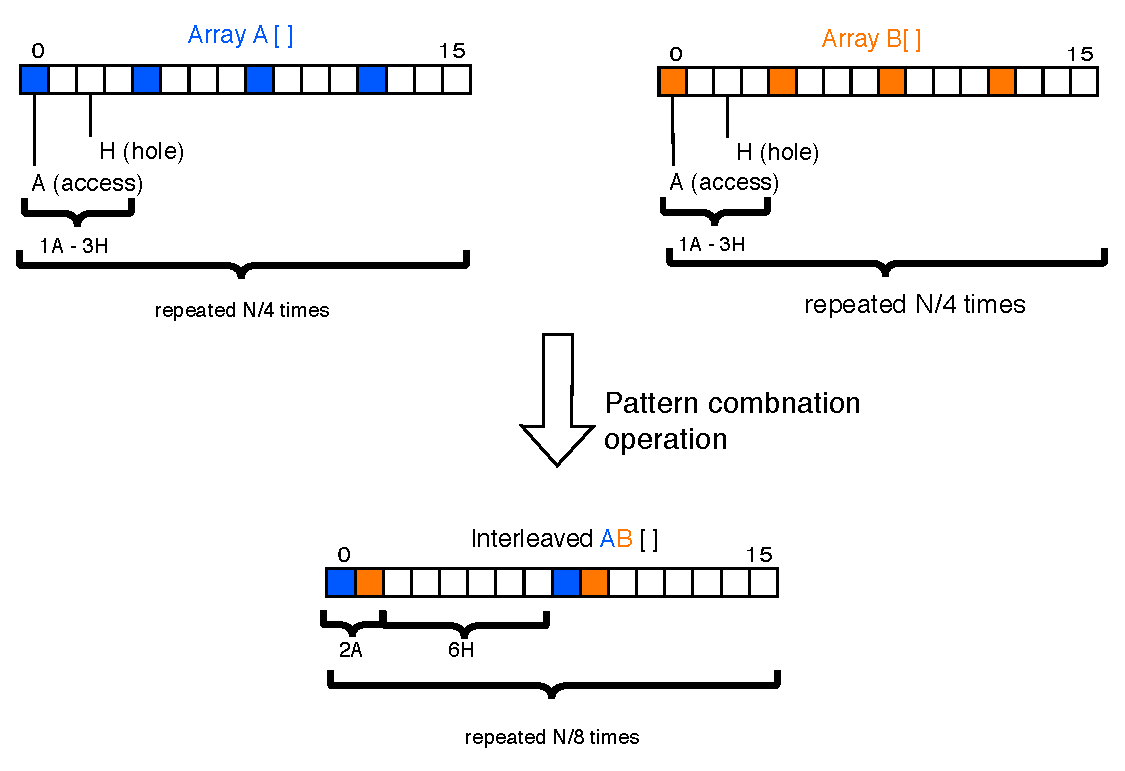
\includegraphics[scale = 0.6]{D/Images/Algebra.eps} 
	\caption{Example of combination between two arrays and their access patterns}
	\label{fig:algebra}
\end{figure}
%\textit{Algorithm for exploring data interleaving}

\subsection{Data-to-Memory Mapping Exploration}

Given the input from the previous step, we explore the mapping of the interleaved data to the memory architecture.
A clustered memory organisation with up to five memory banks of varying sizes is explored. 
The limitation in the number of memory banks is necessary in order to keep the interconnection cost between the processing element (PE) and the memories constant through exploration of different architectures. 
There are two main reasons for exploring architectures up to five memory banks.
Firstly, the energy gains achieved by increasing the number of memory banks in the memory architecture are nearly saturated even for five banks.
In \cite{filippopoulos2013exploration} a group of different applications were studied with regard to their energy consumption on a clustered memory architecture consisting of up to five memory banks.
The results show that depending on the application, the energy gains start to saturate after adding a third or a fourth bank and become insignificant when adding a fifth bank.
Thus, for most applications a memory architecture with five memory banks already provides the necessary reconfiguration options.  
Secondly, the overhead increases exponentially with the number of memory banks, due to the increased complexity of the memory architecture. 
Therefore, memory architectures with six or more banks are typically not efficient options due to the high overhead and the low energy gain.

The decision to use memory banks with varying sizes on the clustered memory organization increases the reconfiguration options and consequently the potential energy gains. 
In general, smaller memories are more energy efficient compared to larger memories banks. 
However, in some cases large memory banks are needed in order to fit the application data without the need for too many small memories causing complex interconnects. 
The goal is to use the most energy efficient banks to store the interleaved data.

The exploration space consists of different sizes and types of memory banks.
The goal is to select the optimal set of memory banks and to make  the optimal decision regarding the mapping of the data to the different memory banks.
The parts of the interleaved data that consist mostly of useful elements are mapped into memory banks with low energy per access but at the same time with the necessary access time.
The parts of the interleaved data that consist of access holes and rarely accessed elements are optimally mapped into memory banks with energy efficient retention states.
In both cases the size of  the memory banks should be adequate to fit the stored data but at the same time as small as possible to avoid area and energy penalties.

\subsection{One way constraint propagation}

The interleaving decisions influence the data-to-memory mapping decisions and vice versa.
For example, the decision to interleave two arrays \textit{A and B} have an impact on the freedom of mapping the interleaved array $A\vert B$ on the memory banks, because of the difference in size and structure.
The data-to-memory mapping decisions affect the interleaving decisions in a similar way.
Assuming that the mapping is performed first using the initial data the following interleaving options are reduced.
For example, the decision to map two arrays on different memory banks removes the option to interleave them later.
Optimizing both the interleaving and the memory mapping at the same time results in a large and inefficient loop of constrain propagations between the two exploration phases.
 
We choose to perform the interleaving exploration step first and then propagate the most efficient interleaving options to the data-to-memory mapping step.
The code and data transformations should be performed earlier to avoid omitting possible solutions as justified in \cite{dtse}.
Thus, the interleaving decisions are propagated as constraints on the mapping exploration phase. 
The constrains consist of the arrays that are interleaved, the new access pattern and the width of SIMD architecture for which the specific interleaving solution is optimal.
The mapping step is performed based on these constrains.

\section{Applications and Experimental Evaluation}
\label{sec:applicationsD}

\subsection{Benchmark Applications}

Array Interleaving is a data layout transformation for combining the storage of multiple arrays, so that blocks of data from different arrays are stored contiguously, with the objective of reducing the number of memory accesses through better spatial locality. \cite{sharma2015array}.
The target applications on the current work benefit most from the proposed methodology, because they are characterized by having access patterns with holes.
Interleaving is a widely used technique that fits the goal of generating more compact sets of data.
An important contribution of the work is the combination of the interleaving optimization with data to memory mapping. 
Another important advantage of interleaving transformations is the low addressing  overhead.
In more detail, interleaving results in a more regular global access by reducing the number of holes without increasing significantly the addressing for accessing the individual arrays afterwards.
Although more complex data layout transformations may reduce the holes in the access patterns even more, they have a negative impact on the complexity of addressing and access overhead.
Having shown the benefits of this, future work can include extending the methodology to be compatible with additional layout optimization techniques.

Applications with holes in their access pattern can be found on several application domains.
The current study includes representative candidates from three different domains, namely the multimedia, the wireless and the equation solver domains.
Suitable applications can also be found on other areas.
An overview of the tested benchmark applications is presented below:

\begin{enumerate}
\item Motivational example is the very simple example presented in Sec.~\ref{sec:motivationalD}. 
It uses four arrays that all have holes in their access pattern, namely 1A-3H.
One element from each array is used to calculate an intermediate result on every loop iteration.
The interleaving is easy because the four arrays have the same pattern.
Further interleaving within the array can result in even longer sequences of useful elements.
The access pattern is repeated for every four elements (1A-3H), so the scaling for the different word lengths (4, 8 and 16) is expected to be good. 
\item Successive Over Relaxation (SOR) is a method for evaluating partial differential equations or solving a linear system of equations.
The SOR benchmark has an access pattern with more holes and different distribution of them.
The interleaving exploration provides sequences of three or six sequential useful elements.
Thus, the utilization on the SIMD architecture is expected to be lower.
This application is a representative example from the equation solver domain.
\item FFT benchmark has holes in the access pattern during the access of the pilot matrices. 
The interleaving exploration for FFT is presented in \cite{sharma2013data}.
The number of matrices is higher and more interleaving options are present.
However, the interleaving cannot provide an acceptable solution for 16 sequential useful elements.
This application is an representative example from the wireless domain, because FFT is widely used on wireless applications.
\item Motion estimation benchmark is a dynamic algorithm that results in different access patterns based on the identification of the moving objects. 
The static parts are not accessed resulting in holes in the accesses and the interleaving aims to minimize those parts.
The interleaving exploration provides alternatives for all the  tested word lengths. 
This application is an representative example from the multimedia domain.
\end{enumerate}

\subsection{Results}
\label{sec:resultsD}

%\begin{table}%
%\tbl{Normalized energy consumption\label{tab:results}}{
%\begin{tabular}{c c}
%\includegraphics[width=0.45\linewidth]{Images/Example.eps} & \includegraphics[width=0.45\linewidth]{Images/sor.eps} \\
%\includegraphics[width=0.45\linewidth]{Images/fft.eps} & 
%\includegraphics[width=0.45\linewidth]{Images/mest.eps} 
%\end{tabular}}
%\end{table}

The design exploration is applied to the chosen application benchmarks and energy numbers are derived based on the described target platform.
The energy numbers are calculated both for the memory and the SIMD architecture presented in Sec.\ref{sec:platformD}.
Four approaches are explored and the corresponding energy consumption for each of them is calculated.

\begin{itemize}
\item \textit{No optimization.} 
In this case there is no interleaving exploration and the memory architecture consists of one large memory bank. All the data are mapped on the memory bank without any optimization. 
\item \textit{Memory Size Optimization.} 
In this case there is no interleaving exploration and the memory architecture consists of five memory banks.
The optimal size for the memory banks and the optimal mapping of the non-interleaved data on them is explored. 
The number of memory accesses is the same as in the previous approach.
However, the data is mapped on an efficient clustered memory architecture.
\item \textit{Interleaving optimization.} 
In this case the  interleaving exploration step is performed and the memory architecture consists of one large memory bank.
The optimal interleaving decision is found and applied to the data, so the locality of useful data is increased.
However, all the data are mapped on one large memory bank.
The number of accesses is significantly reduced by the interleaving step, but the energy per access is kept high due to lack of data mapping to an efficient clustered architecture.
\item \textit{Integrated co-exploration.} 
In this case the co-exploration of both the interleaving and the data-to-memory mapping optimizations is performed.
Both he number of memory accesses and the energy per access are reduced.
\end{itemize}

\subsubsection{Motivational Example}

\begin{figure}
\centering
	\includegraphics[scale = 0.5]{D/Images/Example.eps} 
	\caption{Motivational Example}
	\label{fig:example}
\end{figure}

The normalized energy consumption for the motivational example is presented in Fig.\ref{fig:example}.
The four different approaches are normalized using the monolithic approach without any optimization.
Energy results for this benchmark are presented for a bus width of 4, 8 and 16 elements, which means that every memory access loads/stores 4,8 or 16 elements. 
The interleaving exploration proposes three different solutions for an SIMD architecture width of 4, 8 and 16 elements respectively.
The data access patterns of the three interleaving decisions are propagated as a set of constrains to the mapping step.
The mapping step explores all the different data-to-memory mapping options and proposes the most energy efficient memory organization for each of the three interleaved data solutions.

The application code is perfectly suited for interleaving as discussed in Sec.\ref{sec:motivationalD}.
Thus the interleaving exploration has a greater impact than the memory size optimization.
However, the integrated approach optimizes the energy consumption even further.
The application is suitable for higher bus widths and there are important gains while moving from 4 to 8 and 16.
The increase in the architecture width result in significant gains even without any optimization.
The gains are approximately 50 and 70\% for a width of 8 and 16 compared to a width of 4.
This is explained by the fact that the accessed array elements are close enough even without data transformations and the existence of holes in the access pattern. 
By fetching 8 and 16 elements from the memory, the number of useful elements is two and four times more.
Studying the motivational example in Fig.\ref{fig:example}(a) for a width of 16, each access results in 4 lines with one colored element each.

The interleaving optimization results in greater improvements compared to the memory optimization.
This is explained by the nature of the application that offers good interleaving options for larger words, i.e. higher values of bus width.
The memory optimization is around 20\% lower than the monolithic approach for any width.
The interleaving optimization results in more than 70\% lower energy for a width of 4 and more than 80\% for a width of 8 and 16.
The interleaving of the arrays provides perfectly compact sets of data as shown in Fig.\ref{fig:example} and the interleaving cannot improve more for higher values of width.
The great impact of the combined approach is better illustrated for a width of 16. 
In this case the two optimizations alone report an energy gain around 20\% and 35\% compared to the non optimized case for width of 16.
The combined approach results in an energy gain of 84\% on the same case.

\subsubsection{SOR Benchmark}

\begin{algorithm}
\caption{Code snippet from the SOR benchmark}
\label{alg:sor}
\begin{algorithmic}[1]
\FOR{$j = 0 \to N$} 
	\STATE $...$
	\STATE $resid \gets ... + c(i)(j) \times u(i)(j-1) + d(i)(j) \times u(i)(j) + e(i)(j) \times u(i)(j+1) + ... $
	\STATE $...$	
	\STATE $j \gets j + 2$
\ENDFOR
 \end{algorithmic}
\end{algorithm}

%\begin{algorithm}
%\caption{Code snippet from the SOR benchmark}
%\label{alg:sor}
%\begin{algorithmic}
%%\ldots \\
%%$N \leftarrow 100$ \newline
%%\FOR{$j = 0 \to N$} 
%%	\ldots \\
%%	resid = \ldots \\
%%			+$ c(i)(j) \times u(i)(j-1) $ \\ 
%%			+$ d(i)(j) \times u(i)(j) $ \\
%%			+$ e(i)(j) \times u(i)(j+1) $ \\
%%			+ \ldots \\	
%%	\STATE $j \gets j + 2$		
% %\ldots \\		
%\end{algorithmic}
%\end{algorithm}

\begin{figure}
\centering
	\includegraphics[scale = 0.5]{D/Images/sor.eps} 
	\caption{SOR Benchmark}
	\label{fig:sor}
\end{figure}

The normalized energy consumption for the SOR benchmark is presented in Fig.\ref{fig:sor}.
The four different approaches are normalized using the energy consumption of a system without any optimization as the base.
Energy results for this benchmark are presented for a bus width of 3 and 6, although the architecture supports bus widths of the power of 2.
This means that every memory access loads or stores 4 or 8 elements, but only up to 3 or 6 array elements are used in the algorithm.
This limitation is due to the nature of the application code that adds elements from 3 arrays to 3 sequential elements of another array. 
Alg.~\ref{alg:sor} is a code snippet that demonstrates the considered data structures.
The arrays \textit{c, d and e} are potential candidates for the interleaving exploration.
The interleaving exploration on the application code concludes that it is only possible to make sequential sets of 3 and 6 elements by interleaving the arrays \textit{c, d and e}.
The elements that are multiplied with them are already sequential.

 The interleaving exploration has a small impact on the reduction of energy consumption for a bus width of 3 elements.
 This is due to the addition of a redundant element, in order to have a width of four that is supported by the architecture.
The results are even worse for a bus width of 6 elements, because there is a need for two redundant elements to comply with a set width of eight.
The mapping of the initial data to a clustered memory results in a reduction of around 20\%, which is slightly better than the interleaving optimization.
The reason is that the mapping of the initial data demands all the memory banks active and the memory is heavily accessed during the execution of the benchmark.
The integrated approach exploit on a better way the few interleaving options and provides a better mapping of the interleaved data to the memory architecture.
The final gain for a width of three is 47\%, compared to 17\% and 20\% for the interleaving and the memory optimization respectively.

\subsubsection{FFT Benchmark}

\begin{figure}
\centering
	\includegraphics[scale = 0.5]{D/Images/fft.eps} 
	\caption{FFT Benchmark}
	\label{fig:fft}
\end{figure}

The normalized energy consumption for the FFT benchmark is presented in Fig.\ref{fig:fft}.
The four different approaches are normalized using the monolithic approach without any optimization.
Energy results for this benchmark are presented for a bus width of 4 and 8 elements, which are the two viable options provided by the interleaving exploration.
Again, the integrated approach results in the lower energy consumption.
The energy gains for a bus width of 8 are significant, because blocks of 8 elements can be constructed by interleaving of application's arrays.

\subsubsection{Motion Estimation Benchmark}

\begin{figure}
\centering
	\includegraphics[scale = 0.5]{D/Images/mest.eps} 
	\caption{Motion Estimation Benchmark}
	\label{fig:mest}
\end{figure}

The normalized energy consumption for the motion estimation benchmark is presented in Fig.\ref{fig:mest}.
The four different approaches are normalized using the monolithic approach without any optimization.
Energy results for this benchmark are presented for a bus width of 4, 8 and 16 elements.
The application code provides good possibilities for interleaving and consequently the interleaving exploration has a greater impact than the memory size optimization.
However, the integrated approach optimizes the energy consumption even further.
In this case the energy gains for increasing size of bus width are minimal when only one optimization is applied.
This is explained by the nature of the application, which has large parts of redundant data spread out through the memory.
Thus, the whole memory is active when the mapping is not performed on the compact interleaved data.
The combined approach offers significant energy gains even for the highest bus width. 

\section{Conclusion}
\label{sec:conclusionD}

The scope of this work is to presents a methodology for efficient exploration of data interleaving and data-to-memory mapping options for SIMD (Single Instruction Multiple Data) platform architectures.
Detailed energy models are presented for the studied architecture.
The methodology focuses on reducing the overall energy consumption by reducing the number of memory accesses and the energy per access.
The number of memory accesses is reduced by interleaving the application data to construct compact sets of sequential data.
The energy per memory access is reduced by employing a reconfigurable scratch-pad memory architecture with multiple banks that can operate independently.
A systematic way is presented in order to explore the different options that lead to the interleaving and data-to-memory mapping decisions.
A wide range of applications is studied that allow us to draw conclusions about different kinds of dynamic behavior and their effect on the energy gains achieved using the methodology. 
The improvement in the total system energy consumption after efficient interleaving and mapping of data is between 40\% and 80\% for the studied benchmarks having the type of holes in their access scheme that benefit most from the methodology.

% Bibliography
%\addcontentsline{toc}{section}{Bibliography}	
%\bibliographystyle{plain}
%\bibliography{reference}
%\bibliographystyle{ACM-Reference-Format-Journals}
%\bibliography{reference}

%\documentclass[12pt,a4paper]{article}
%\usepackage[latin1]{inputenc}
%\usepackage{amsmath}
%\usepackage{amsfonts}
%\usepackage{amssymb}
%\usepackage{graphicx}
%\author{Iason Filippopoulos \and Francky Catthoor \and Per Gunnar Kjeldsberg}
%\title{Technology scaling impact on the interconnect of clustered scratchpad memory architectures}

%\begin{document}
%\maketitle


\chapter{Technology scaling impact on the interconnection of clustered scratchpad memory architectures}
\label{interconnection}

\begin{center}
Iason Filippopoulos, Francky Catthoor, Per Gunnar Kjeldsberg
\\
Technical report
\\
2015
\end{center}
\afterpage{\null\newpage}
\newpage

\vspace*{\fill}
\phantomsection
\section*{\hspace*{\fill} Abstract \hspace*{\fill}}
\addcontentsline{toc}{section}{Abstract}
Power consumption is a key limiting factor in modern embedded devices.
The memory architecture contributes significantly to the overall power consumption of the system.
Among many proposed techniques, one effective system design approach to reduce the memory power needs is the design of a dynamically reconfigurable clustered memory architecture.
The operationally independent memory banks provide an energy efficient platform, but come with an interconnection overhead due to the connections between the memory banks. 
Thus, there is a trade-off between the energy gains by increasing the number of memory banks and the increase in interconnection overhead.
This work explores the future development of the interconnection overhead, as the interconnection cost is expected to increase while the process technology shrinks to 5nm.
The current study employs both CAD \nomenclature{CAD}{computer aided design} tools with simulation results using the current technology and projections provided by institutions.
We use predictive technology models supported by information from ITRS and IMEC's interconnect technologists.
A model is developed that provide a sufficiently accurate estimate of the interconnection cost overhead for clustered memory architectures consisting of two to five memory banks in technologies ranging from 40nm to 5nm.  
The model shows that the interconnect overhead is as low as 10.9 \% even for the most aggressive technologies. Hence a dynamically reconfigurable clustered memory architecture is a viable solution also for future designs, even if the optimal number of memory banks may be reduces as shown in an experiment with a representative real life application.
\vspace*{\fill}
\afterpage{\null\newpage}
\newpage

\section{Introduction}

Embedded systems normally rely on battery and their lifetime between charging is limited and dependent on the energy usage of the system.
The power consumption can be divided between the processing elements and the memory subsystem.
One efficient way to reduce the power consumed in the memory, when executing an application with dynamic memory needs, is to design a clustered memory architecture.
A study of the efficiency and the potential gains of this approach is presented in \cite{filippopoulos2013exploration}.
In Fig. \ref{fig:platformE} the two different approaches are presented.
Alternative 1 to the left has a large static memory while Alternative 5 to the right has five smaller memory banks. The designer can choose other alternatives in between.
The different memory banks can operate independently and  adjust to the application requirements.
When the memory requirements of the application are small, unused memory banks can be switched off to reduce the energy consumption, while the application still runs successfully on the system. 
 
 The main drawback of the clustered memory architecture approach is the need for extra interconnection circuitry.
 Unfortunately, it is expected that the interconnection networks will take up an increasingly significant portion of system power in the future. 
Thus, there is a need to obtain a detailed memory and interconnect energy model including the scaling impact. 
That will allow us to accurately incorporate the interconnection cost overhead in our studies to decide whether and when the power gains justify the use of a clustered memory architecture instead of a monolithic one. 
It especially also allows to identify the best trade-off working points between using more
or less memory banks within the clustered approach. 
Without this, an overly optimistic distribution across too many banks would seem to provide the best energy for a given application requirement.
  
  The scope of this work is to explore the future development of the interconnection overhead and develop a model that can provide a sufficiently accurate estimate of that overhead.
  System designers could use such a model to find the preferred memory architecture and the number of banks given the nature of the executed application and the target technology.
  The model is based on the current technology and available projections about the future technology.
  The current technology is available as libraries in CAD tools.
  The synthesis and the simulation of memory architectures similar to the one in Fig. \ref{fig:platformE} provide useful results.
  The study of the future technology is based on the reports released by the International Technology Roadmap for Semiconductors (ITRS) \cite{itrs} \nomenclature{ITRS}{international technology roadmap for semiconductors}.
 The goal of the developed model is to provide a sufficiently accurate estimate of the interconnection cost overhead for clustered memory architectures consisting of two to five memory banks and a range of technologies from 40nm to 5nm.  

%%%%%%
   The studied memory architecture is targeted to applications that significantly increase their energy efficiency when they are mapped on clustered memory architectures.
  These applications are characterized by having dynamic utilization of the memory organization during their execution. 
 Suitable dynamic applications are available on several different domains.
 For example, a set of multimedia applications, which exhibit such a dynamic variation in memory requirements during their lifetime, is presented in \cite{filippopoulos2013exploration}.
 A similar clustered architecture is employed in \cite{Fil12} for a bio-medical application as a suitable example.
 In general, smaller memories are more energy efficient compared to larger memory banks \cite{steinke2002assigning}. 
 The distribution of data into the memory banks should allocate the most frequently accessed data to the most energy efficient memory banks, in order to maximize the potential gains.
 
The paper is organized as follows.
Section~\ref{relatedE} surveys related work on on-chip interconnection with a focus on energy consumption and presents research work on technology scaling. 
Section~\ref{Current} presents the chosen synthesis work-flow and results for the target architecture using the current technology.
In Section~\ref{future} the scaling projections for the different parts of the target architecture are presented.
The development of a model that can provide a sufficiently accurate estimate of the power overhead for the interconnection in clustered memory architectures is presented in Section~\ref{resultsE}.
Finally, conclusions are drawn in Section~\ref{conclusionE}.

\begin{figure}
 \centering
 \includegraphics[width = \textwidth]{E/platform.pdf}
  \caption{The alternative clustered memory architectures ranging from one to five memory banks}
 \label{fig:platformE}
 \end{figure}

\section{Related Work}
\label{relatedE}

A comprehensive view of a class of interconnect architectures is presented in \cite{kumar2005interconnections}. 
The authors examine the area, power, performance, and design issues for the on-chip interconnects.
The main finding is that the interconnect should not be independently optimized but co-designed with the other components, i.e., memories and cores, in order to arrive to the best platform design.
In \cite{rahimi2011fully} authors propose an interconnection network with high-performance for the communication between processors and memories in a cluster of processors.
Another approach that focuses on the interconnection network between the memory and the processing cores is presented in \cite{kang2012high}. 
The majority of the published work focuses on the interconnection between the processing cores in a system-on-chip.
The current work differentiates by focusing on the interconnection between the memory banks.

Several examples of clustered memory architectures have been proposed.
In \cite{cho2009adaptive} an adaptive scratch-pad memory is successfully used in order to handle the dynamic behavior of multimedia applications.
In \cite{wang2005energy} a clustered memory architecture is employed and an algorithm is developed, which efficiently uses the memory banks to achieve the maximum energy saving while satisfying the given performance constraint.
Our approach explores the effectiveness of similar architectures into the future, which is not studied before to the best of our knowledge.

A comprehensive memory modeling tool and its application to the design and analysis of future memory hierarchies is developed in \cite{thoziyoor2008comprehensive}. 
This tool uses the CACTI model and targets large general purpose DRAM and SRAM memory designs.
However, the current work focuses on small scratch-pad memory designs, which cannot be successfully covered by the CACTI model.
A circuit level analysis of the interconnect delay from the 10 nm node to the 7 nm node is presented in \cite{pan2014system}.
The authors in \cite{chen2014interconnect} analyzes the impact of interconnect variation at the system-level in terms of clock frequency based on a fast and efficient system-level design methodology. 
The current work differentiates by focusing on the energy impact and providing a high-level prediction model.

\section{Current technology}
\label{Current}

\subsection{Generic Work-flow}

The current technology is studied as a first step towards the development of an interconnection cost model. 
CAD tools allow the design of the described clustered memory architectures.
The synthesis and the simulation provide reliable data for the area and the power consumption of the different parts of the memory architecture.
The goal is to synthesize a clustered memory architecture and extract power data for the memory banks and the interconnection logic separately.
The work-flow is divided in several sub-steps:

\begin{itemize}
	\item A number of memory banks is chosen from a library, which contains several state-of-the-art designs.
	\item An RTL description for connecting the memory banks into a full memory architecture design is written.
	\item A simulation is performed to verify the correct functionality of the memory architecture.
	\item A target technology is chosen and the logic synthesis of the memory architecture is performed.
	\item Floor-planning and the place \& rout of the memory design is performed.
	\item Dynamic timing and the power simulation are performed and results are provided.
\end{itemize}

The memory models applied in the first step are presented in \cite{filippopoulos2013exploration}.
They are part of a library of standard cell-based memories (SCMEM) designed at IMEC. As shown in \cite{Mei11} such memories are power efficient when the size requirements are small.
The SCMEM used in the current work are developed in IMEC and have similar characteristics with the ones described in \cite{Mei11}.
The energy numbers for SCMEM are derived from synthesis and simulation results.
The presented work-flow is a typical procedure followed by an industry designer except for the usage of SCMEM instead of commercially available memory macros.
SCMEM are preferred for their characteristics,  especially their energy and area efficiency for reasonably small storage capacities, as argued in \cite{Mei10}. 
Thus, the choice of using SCMEM is mostly related to the heavily distributed memory organization, which we target. 
The sizes of the memory banks in the target memory organization are too small to motivate a solution based on macro memory blocks, mainly because macro memories are dominated by the periphery.
Another factor for this decision is that a rectangular cell array is not necessarily the optimal solution in terms of energy consumption.
The usage of the custom memories provides the freedom to explore different memory organizations by combining banks of different sizes and structures.  

For the second step, the RTL description connects the memories using MUX \nomenclature{MUX}{multiplexer}, signals, and other components into a functional clustered memory architecture. 
In the third step, verification is performed through simulation where a flash-write followed by a read on the whole memory architecture is performed. 
The read and write test-bench is representative for the types of data-intensive applications that benefit the most from clustered memory architecture. 
The target technology depends on the available libraries.
In this work, a TSMC \nomenclature{TSMC}{Taiwan semiconductor manufacturing company} 45 nm library is used.
Place and route can either be performed automatically through the CAD tool or manually by the designer.
In our case, the layout is automatically generated to reduce the needed time and effort. 
However, the automatically generated layout is not ideal and a manual layout can be more efficient.
The performance of the layout generation deteriorates for larger memory designs, so in the current work the clustered memory architectures are based on small memory banks.
Although the layout could be improved further manually by the designer, all the designs are generated in the same way and the comparison between them, which is the main focus of this work, can give reliable results.


The final step includes extraction of  parasitic, static timing analysis, and annotation of the timing to the netlist.
Afterwards, power simulations on the synthesized design are carried out using Synopsys PrimeTime, in order to obtain energy numbers.
The access pattern for the simulation consists of one full write of the memory architecture, followed by one full read and the comparison of the written and read data to verify that the memory operates correctly.
Although both the dynamic and static power are reported, the focus of this work is on the dynamic part.
The memory architecture is heavily accessed for the studied data-intensive applications, thus the dynamic power is dominant.
The leakage is higher inside the memory banks than the interconnection, but in both cases significantly lower than the corresponding dynamic part.

\subsection{Example design: synthesis and simulation}

\begin{figure}
 \centering
 \begin{minipage}{0.9\textwidth} % choose width suitably
 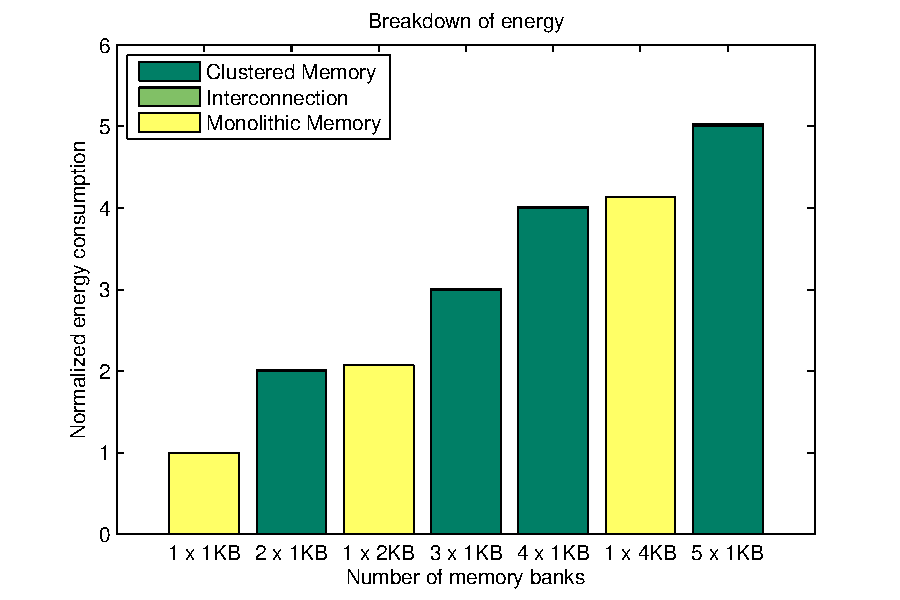
\includegraphics[width =\linewidth]{E/energy2.pdf}
 {\footnotesize Note: The small interconnection overhead is not easily visible in the figure without zooming in the top of the bars.\par}
\end{minipage}
  \caption{Normalized energy breakdown between the memory banks and the interconnection.}
 \label{fig:energyE}
 \end{figure}


A group of clustered memory architectures is designed and synthesized following the presented work-flow.
The simulation provides results for the current technology and the contribution of the interconnection to the overall energy consumption.
The study includes clustered memories with an increasing number of memory banks, beginning with only one memory bank and having five memory banks as the maximum.
There are two main reasons for exploring architectures up to five memory banks.
The energy gains achieved by increasing the number of memory banks in the memory architecture are nearly saturated even for five banks.
In \cite{filippopoulos2013exploration} a group of different applications were studied with regard to their energy consumption on a clustered memory architecture consisting of up to five memory banks.
The results shows that depending on the application, the energy gains start to saturate after adding a third or a fourth bank and become far smaller when adding a fifth bank.
Thus, for most applications a memory architecture with five memory banks already provides more than necessary reconfiguration options.  
Secondly, the interconnect overhead increases exponentially with the number of memory banks, due to the increased complexity of the memory architecture. 
The significant increase in the overhead is indicated by the synthesis results, especially while comparing the overhead between four and five memory banks.
Therefore, a memory architecture with six banks seems to be a less efficient option due to the high overhead and the very low energy gain.
However, further investigation is proposed as future work to provide accurate numbers for architectures with six memory banks.

\begin{table}
\caption{Normalized energy breakdown between the memory banks and the interconnection}
\label{tab:overhead}
\centering
\begin{tabular}{|c|c|c|c|}
\hline 
\parbox{0.2\textwidth}{\centering Memory Configuration} & 
\parbox{0.2\textwidth}{\centering Energy on Memory Banks} & 
\parbox{0.2\textwidth}{\centering Energy on Interconnection} & 
\parbox{0.2\textwidth}{\centering Interconnection Overhead} \\
& & & \\
\hline 
1 x 1KB &  1 & - & 0\% \\ 
 \hline 
2 x 1KB & 2 & 0.03 & 1.26\% \\ 
 \hline  
1 x 2KB & 2.07 & - & 0\% \\ 
 \hline 
 3 x 1KB & 3 & 0.04 &1.37\% \\ 
 \hline 
 4 x 1KB & 4 & 0.07 & 1.77\% \\ 
 \hline 
 1 x 4KB & 4.14 & - & 0\% \\ 
 \hline 
 5 x 1KB & 5 & 0.15 & 3.01\% \\ 
 \hline 
 %1 x 8KB & 8.2768 & - & 0\% \\ 
 %\hline 
 \multicolumn{4}{|c|}{The energy is normalized to a memory bank of 1KB} \\ 
 \hline 
 \end{tabular} 
\end{table} 

The breakdown of energy consumption in the memory architecture is split into two parts.
The first part is the energy consumption internally in each memory bank, which includes the memory cells and the necessary logic to connect the cells.
The second part is the interconnection cost between the different memory banks, which includes the necessary logic to locate and transfer the data outside of the banks. 
In other words, the interconnection outside the memory banks is given separately. 
The interconnection between the different memory cells inside one bank is included in the energy of the memory bank.

 \begin{figure}
 \centering
 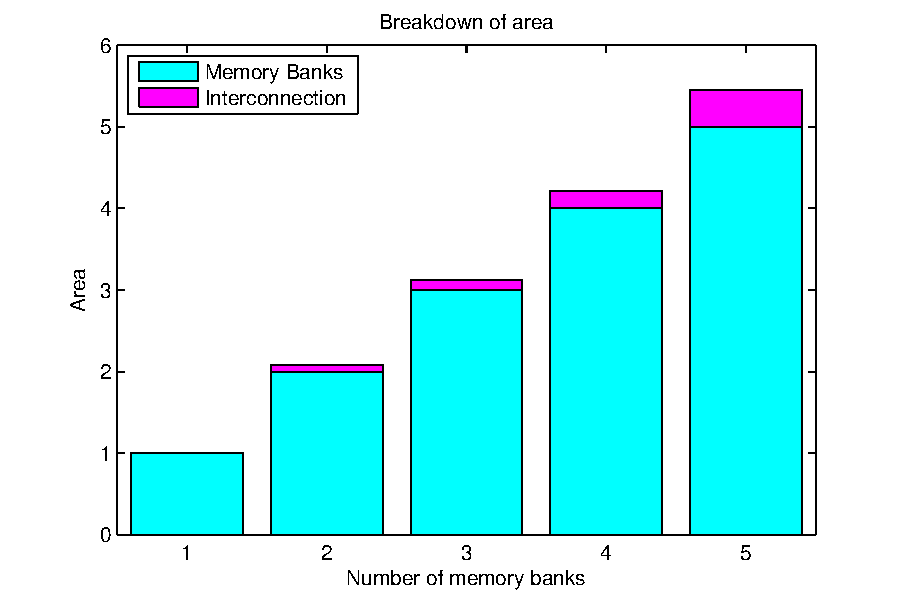
\includegraphics[width = 0.9\textwidth]{E/area.pdf}
  \caption{Normalized area breakdown between the memory banks and the interconnection}
 \label{fig:areaE}
 \end{figure}

The example design is built using memory banks of 1KB and a bus width of 32bits.
Each bank has one read and one write port and can operate independently.
The memory banks are not directly connected to each other, but connect to a multiplexer that can read and write data to the appropriate bank based on the data address. 
The energy breakdown between the first part of the memory banks and the second part of the interconnection (part2) is presented in Fig. \ref{fig:energyE}.
The energy cost of the interconnection logic is very small compared to the energy cost for the write and read operations on the memory banks.
Tab. \ref{tab:overhead} contains the exact percentages of the energy overhead of the interconnection. 
Energy consumption for a monolithic design with only one large 4KB memory is included in Fig. \ref{fig:energyE}.
The comparison shows that the energy consumption for this design is higher than in a clustered solution with four 1KB memories, although there is no need for interconnection logic.
This is due to the fact that the energy consumption for each access operation increases with the size of the memory \cite{steinke2002assigning}.
 
The changes in memory area for the designs are presented in Fig. \ref{fig:areaE}.
The area used for the placement of the memory banks is separated from the area occupied by the interconnection.
The overhead calculation for additional banks takes into consideration the increase in the interconnect and the increase in address decoding and all other necessary design modifications.
The last column corresponds to the area footprint for a monolithic 4KB memory.
The area footprint for placing 4 banks of 1KB is larger than the area for one bank of 4KB.
The higher area is needed for the interconnect. Furthermore, the layout is easier and more compact when there is only one bank of 4KB.
A manual layout can potentially reduce the area overhead for the clustered memory, but this is beyond the scope of this work.

In addition, the synthesis and simulation of the memory designs provide useful information about the dimensions of the memory banks, the length and the capacitance of the wires.
Several interesting observations are possible based on the study of the current technology.
The energy overhead caused by the interconnection of the banks grows when there are more memory banks connected, as expected.
However, the overhead is only slightly over 3\% even for a clustered memory with five banks. 
The area overhead is significantly higher and grows exponentially for an increasing number of memory banks.  
The maximum area overhead is still below 10\%.
This is explained by the need for extra wiring to connect the different memory banks.
Again, it should be noted that the results are for the dynamic power. Static power is omitted due its low contribution in the interconnection and the data intensive behavior of the target applications. 

\section{Technology Scaling}
\label{future}

The technology scaling projections are based on the reports released by the International Technology Roadmap for Semiconductors (ITRS)  \cite{itrs}.
The clustered memory architecture can be divided into two parts, the memory banks and the interconnection.

\subsection{Memory Banks}

\begin{figure}
 \centering
 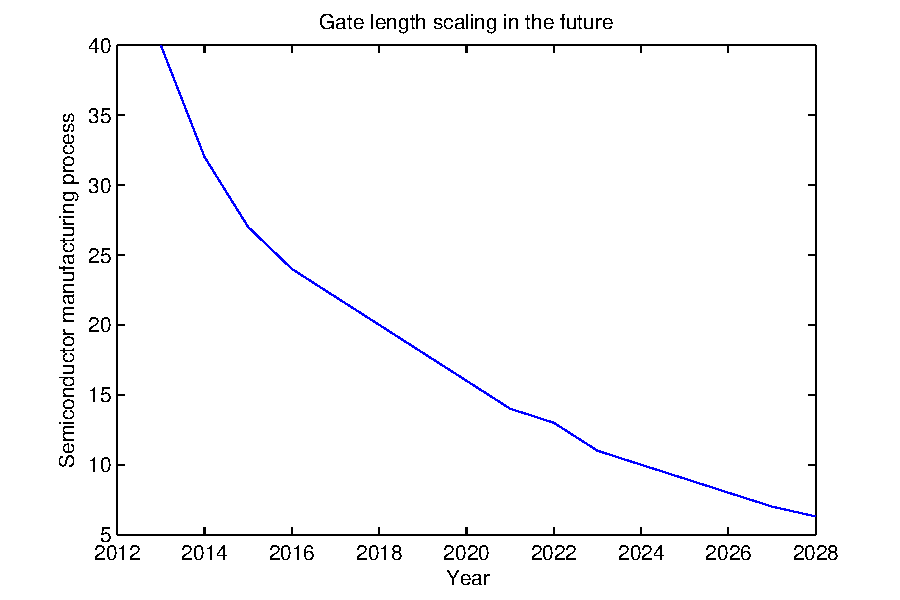
\includegraphics[width = 0.9\textwidth]{E/gate.pdf}
  \caption{Impact of technology scaling into gate length}
 \label{fig:gateE}
 \end{figure}
 
The memory banks consist of the memory cells, which in our case are built using gates.
Thus, the predictions about the future behavior of the memory banks are based on the ITRS reports for logic.
The reports for logic are chosen, because the clustered memory architectures that are studied in this work are synthesized using standard cells.
Different predictions and reports are provided by ITRS for other types of memories, such as DRAM.
However, the proposed scratchpad memory architectures are the preferred choice for our scope.
Typically the memories used in embedded systems are smaller and more energy efficient than DRAM.

In the coming years, the transistor gate length is expected to be reduced as shown in Fig. \ref{fig:gateE} generated from data found in \cite{itrs2}.
The values are approaching 5nm around 2028, which is potentially the limit using the current manufacturing process.
The reduction in gate lengths leads to a reduced size of the memory cell and consequently smaller memory banks.
The smaller memory banks affect both the area of the design and the power consumption.
The projections provided by ITRS regarding the power are presented in Fig. \ref{fig:powerE} generated from data found in \cite{itrs2}. 
There is a significant reduction in power consumption in the short term and slighter reduction towards the end of the projections.

  \begin{figure}
 \centering
 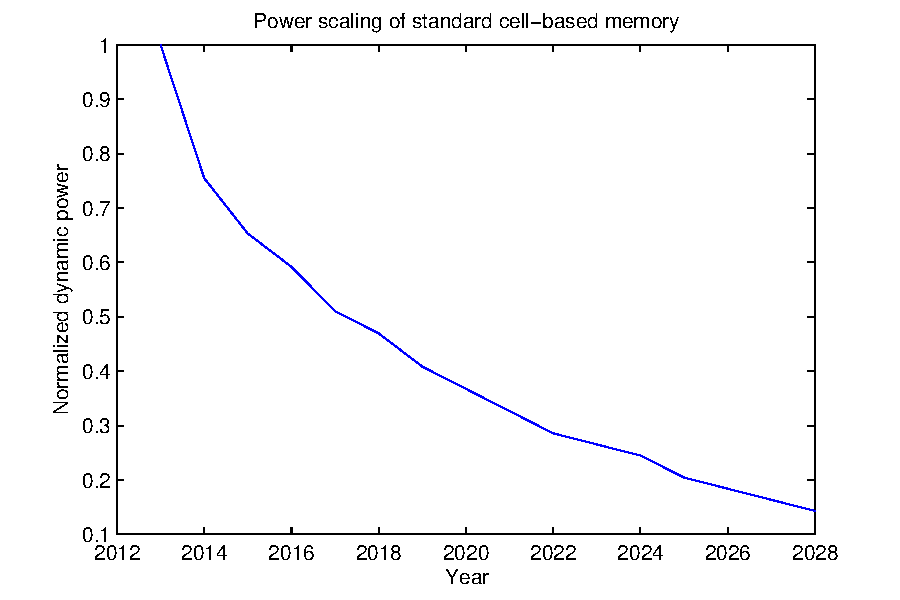
\includegraphics[width = 0.9\textwidth]{E/cellpower.pdf}
  \caption{Memory Banks: Normalized dynamic power and technology scaling}
 \label{fig:powerE}
 \end{figure}

\subsection{Interconnection}

The interconnection cost is based on the projections about wiring, which are different from the projections for logic gates.
The current study is restricted to the reports about the lower and intermediate metal layers, because these are the ones that are relevant for the interconnection of our memory organizations.
The reports about the global interconnection scaling is not our focus, as it is used for the power and clock routing and between computing clusters on large SoC platforms.
However, the changes in size of the memory banks affects the length of the needed wires.
The most important parameters for the current study are the capacitance and the power consumption of the interconnection.
Curves for these two parameters are presented in Fig. \ref{fig:intpowerE} generated from data provided by ITRS \cite{itrs2}.
The capacitance is expected to be reduced in the following year.
Although the capacitance is reduced, the rate of this reduction is lower compared to the expected reduction for the memory cells.
The power values are per length unit and they are expected to rise due to several challenges that the interconnection technology will face in the future.

 \begin{figure}
 \centering
 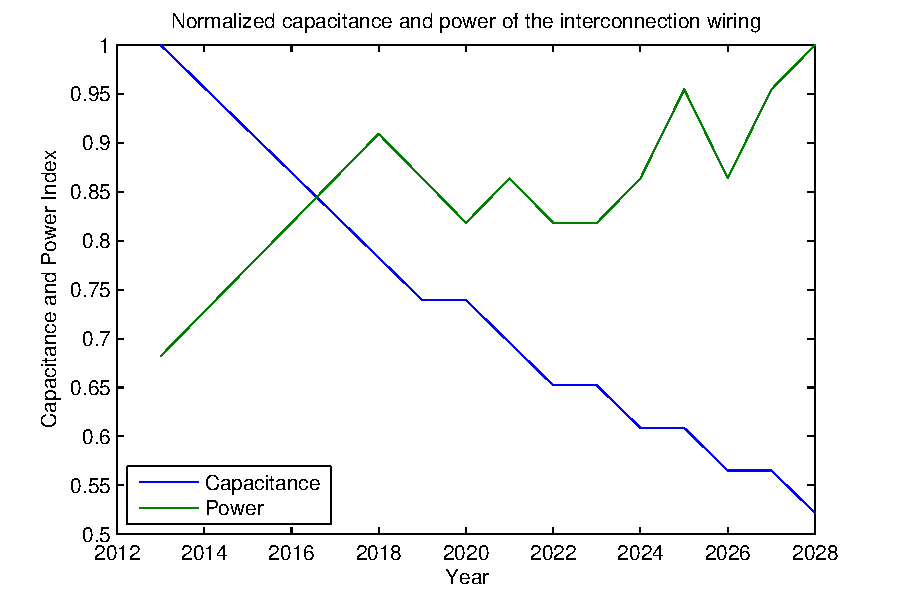
\includegraphics[width =0.9\textwidth]{E/intpower.pdf}
  \caption{Interconnection: Impact of technology scaling on the capacitance and the power consumption of the interconnection part}
 \label{fig:intpowerE}
 \end{figure}
 
The significant parameter in this work is the capacitance.
Resistance is also generally studied in the interconnection because of its important impact, especially for signal
delay. 
The current work focus on energy rather than delay and this is a rational choice for embedded systems.
In general, the clock speeds are relatively low for a typical embedded system in contrast to high performance computing.
In our target domain, a system architecture includes several processing cores that can be of different types to fulfill different application requirements.
When higher performance is needed in an embedded system, it is usually achieved by adding another processing core or a special hardware unit rather than having an extremely high clock speed.
Thus, it is expected that the critical path delay is not the main worry for a system designer.
If the aim is high-performance designs, the current work has to be extended in the future.
A different approach where delay-energy trade-offs are incorporated
from the start should be developed in such a case. The interconnect resistance would then be important in addition to the capacitance.

\section{Model Construction and Projection Results}
\label{resultsE}

\subsection{Model Construction}

 The scope is to develop a model that can provide a sufficiently accurate estimate of the power overhead for the interconnection in clustered memory architectures.
 The model is based on synthesis results of feasible designs in current technologies and study of the projections provided by ITRS.
 The model focuses on the dynamic power, which is the dominant factor for data intensive applications.
 Although leakage power is increasing for smaller technology nodes, the effect on the proposed clustered architecture is low.
 The main reason is that the part of the memory that is active at a given time is heavily accessed for the target applications, thus the static power is negligible compared to the static power.
 The part of the memory that is not accessed at a given time is normally switched off, thus the static power is heavily reduced. 
 The study of the dynamic power is hence sufficient within our scope.
 The interconnect static power is generally low compared to the memory banks as discussed in \cite{liu1994power}.
 
 The input for the model is the process technology and the configuration of the clustered memory architecture.
 The process technology leads to different points in Fig. \ref{fig:powerE} and Fig. \ref{fig:intpowerE} for the memory banks and the interconnection respectively.
 For the ITRS predicted year of a given technology on the x-axis chosen, the corresponding normalized values for dynamic memory power, interconnect capacitance and power can be found. 
 The configuration of the architecture reveals the number of memory banks and all widths and lengths of the memory configuration.
 The power consumed by the memory banks is calculated using the total number of memory cells:
 \begin{center}
 $$ Banks_{power} \propto \sum_{Banks}^{for all} W \times L \times Cell_{power} $$
 \end{center}
  where $W$ and $L$ is the width and the length of each memory bank measured in memory cells. 
  The power per cell is extracted using Fig. \ref{fig:powerE}.
  Each technology node year on the x-axis, leads to the corresponding cell power on the y-axis.

  
 The prediction of the power consumption on the interconnection logic is based in Fig. \ref{fig:intpowerE} in a similar way.
 Based on the technology and the number of memory banks, the length of the wires is calculated, which again gives the power and the capacitance.
 The general formula for the power consumption on a wire is:  
 \begin{center}
 $Power = \dfrac{1}{2} \times f \times C \times V^{2} $
 \end{center}
 where  $f$ is the activity factor, $C$ the capacitance and $V$ the supply voltage.
 However, the simulation results and the projections provided by ITRS suggest that a more detailed model is needed. 
 The basic principle for the model is that the overall interconnection power is proportional to the power of the wires and their capacitance, as explained in  the model presented in \cite{wong2000modeling} and justified on the interconnection study in \cite{muralimanohar2007interconnect}.
 Thus, the general formula for the interconnection power is:
 \begin{center}
 $$ Interconnection_{power} \propto Area(W,L) \times Wire_{power} \times Capacitance $$
 \end{center}
 where $Area$ is calculated based on the total width and length of the memory banks according to the selected configuration.
  In more detail, the different memory banks are placed in a structure similarly to the configuration presented in Fig. \ref{fig:platformE}.
  The library of memory banks provides all the necessary information regarding their sizes.
  The simulation results for the synthesized configurations provide a sufficiently accurate estimate of the area needed for the interconnection, given the number and the sizes of the memory banks.
 The model for the interconnection power cost overhead for a given target technology $ t $ is given by the $ Banks_{power}$ and the $ Interconnection_{power}$:
 \begin{center}
 $$ Overhead = \dfrac{Area(W,L) \times Wire_{power}(t) \times Capacitance(t)}{\sum_{Banks}^{for all} W \times L \times Cell_{power}(t)} $$ 
  \end{center}
 where 
 \begin{itemize}
 \item $ Wire_{power}(t) $ is the wiring efficiency factor based on the power curve in Fig. \ref{fig:intpowerE}
 \item $Capacitance(t)$ is the capacitance of the interconnection wires for the given technology and the length of wiring based on the area, which is calculated for the different number of banks
 \item $Cell_{power} $ is the power consumption of a memory bank for the given technology
 \end{itemize}
 The model is an approximation of the interconnection overhead and the goal is to produce results for relative comparison. 

 The development of the interconnection cost overhead using the proposed model is presented in Fig. \ref{fig:overheadE}.
 The interconnection overhead is kept below 10\% for most of the cases.
 It exceeds this limit in designs with 5 memory banks around a decade from now.
 As expected, the overhead increases as we move from 2 towards 5 memory banks.
 However, the increase is much higher between a design of 4 and 5 memory banks compared to the smaller configurations.
 As motivated before, a memory architecture with six banks is not presented due to the expected high overhead that cannot be justified with the reconfiguration energy gains.
 The interconnection overhead predicted by the model is compared with the synthesis results for the current technology.
 In Tab. \ref{tab:verification} the first column is the overhead percentage presented in Tab. \ref{tab:overhead} and the second column the predicted overhead percentage presented in Fig. \ref{fig:overheadE}.
 The agreement between the two suggests that the model is sufficiently accurate for the current technology.
 
 \begin{center}
	\begin{table}
	\caption{Comparison between predicted and simulated overhead}
	\label{tab:verification}
	\centering
	{
	\begin{tabular}{|c|c|c|}
	\hline
	Number of Banks &	Simulated Overhead & Predicted Overhead \\
	\hline
	2 & 1.26\%  & 1.16\% \\
	\hline 
	3 & 1.37\%  & 1.26\% \\
	\hline 
	4 & 1.77\% & 1.63\% \\
	\hline
	5 & 3.0\% & 2.78\% \\
	\hline	
	\end{tabular}}
	\end{table}
\end{center}

 \begin{figure}
 \centering
 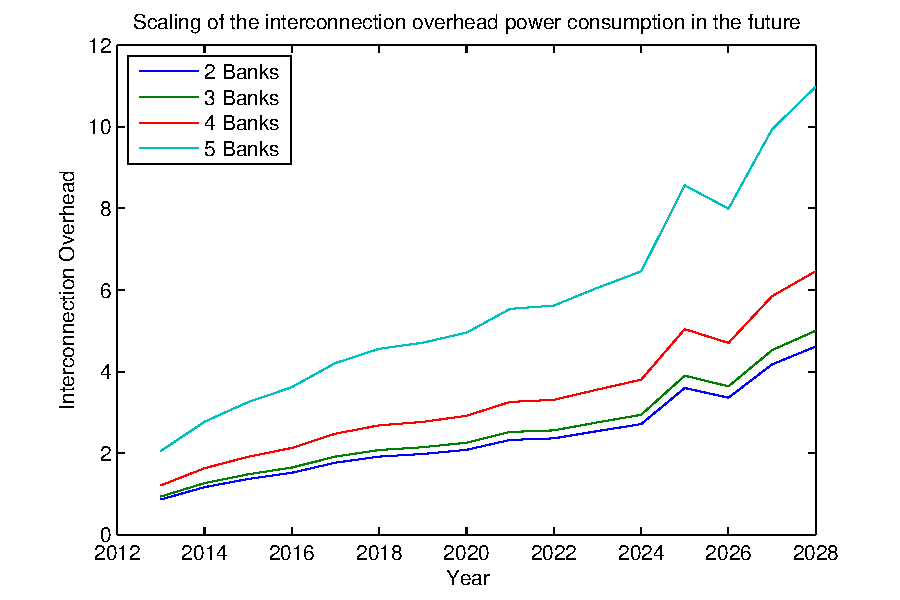
\includegraphics[width = 0.9\textwidth]{E/overhead.pdf}
  \caption{Projections of the interconnection cost power overhead for different numbers of memory banks}
 \label{fig:overheadE}
 \end{figure} 

 
\subsection{Results}
 
The model is useful during exploration of efficient clustered memory organization for a given application and technology. 
Based on Fig. \ref{fig:overheadE} it is likely that the optimum memory organization for a 45 nm design will include more memory banks compared to a 5 nm design.
The overall results also indicates that since the overhead is small, the design approach using clustered memory architectures will be relevant in the future.
The model provides necessary information to the system designer and steers the decision about the number of banks in the memory architecture for a given technology.
The improvement in the designer's decision is a strong motivation for the development of the model. 

To better illustrate the change in the optimum memory architecture for future technologies, an example application is chosen.
The EPIC (Efficient Pyramid Image Coder) \nomenclature{EPIC}{efficient pyramid image coder} is an image compression algorithm and its behavior on a clustered image architecture is presented in \cite{filippopoulos2013exploration}.
The energy gains for the most energy efficient memory organizations are presented in Tab. \ref{tab:GainvsOverhead}. In these numbers the cost of the added interconnect is not included.
The energy gain percentage is constant and independent of the technology, because the comparison is always between a monolithic and a clustered memory architecture of the same technology.
The sizes of the memory banks for each configuration are used to calculate the interconnection overhead for synthesizing in 45nm and 5nm.
The percentage of the energy overhead due to the interconnection cost is also presented in Tab. \ref{tab:GainvsOverhead} both for the current and the most advanced technology.
Based on the improvements and the overheads the most energy efficient design for a specific technology can be defined for the EPIC benchmark application.
For the 45nm technology, a clustered memory architecture with five memory banks is the optimum, while for the 5nm technology four memory banks give the optimal solution.
The addition of a fifth bank reduces the energy consumption by 2.7\%, as a result of the lower energy consumption inside the memory banks, but at the same time increases the energy consumption by 4.5\%, as a result of the higher energy consumption on the interconnection between the banks.

\begin{center}
	\begin{table}
	\centering
	\caption{Energy gains vs. interconnection overhead}
	\label{tab:GainvsOverhead}
	{
	\begin{tabular}{|c|c|c|c|c|}
	\hline
	Banks & Sizes [kB] & Gains & Overhead(45nm) & Overhead(5nm) \\
	\hline
	2 & 8/32 & 40.1\%   & 0.8\%  & 4.6\%  \\
	\hline 
	3 & 8/8/16 & 47.6\%   & 0.9\%  & 4.9\% \\
	\hline 
	4 & 8/8/8/8 & 51.7\% & 1.2\% & 6.4\% \\
	\hline
	5 & 2/8/8/8/8 & 54.4\% & 2.0\% & 10.9\% \\
	\hline	
	\end{tabular}}
	\end{table}
\end{center}
  
\section{Conclusion}
\label{conclusionE}

We have proposed a model that can provide estimates of the interconnection overhead in a clustered memory architecture in future technology nodes.
The model suggests that overhead will be kept low in the short term and will increase within reasonable levels in the mid-long term.
Therefore, the design of energy efficient clustered memory architecture will continue to be a good design choice.
The estimations for the future can be useful for system designers that try to design power efficient architectures for applications with dynamic memory requirements throughout their lifetime.
Another contribution of the model is that it provides an early indication about the optimal number of banks for a given technology and design.
This information reduces the design space exploration and the design time. 
When newer technologies become available in the CAD tools, the designs can be re-synthesized and the model can be calibrated.

\addcontentsline{toc}{section}{Bibliography}	
\bibliographystyle{plain}
\bibliography{reference}

%\end{document}

\chapter{Systematic Exploration of Power-Aware Scenarios for IEEE 802.11ac WLAN Systems}
\label{dsd}

\begin{center}
Nikolaos Zompakis, Iason Filippopoulos, Per Gunnar Kjeldsberg, Francky Catthoor and Dimitrios Soudris
\\
17th Euromicro Conference on Digital System Design (DSD) 
\\
IEEE
\\
2014
\end{center}
\afterpage{\null\newpage}
\newpage

\vspace*{\fill}
\addcontentsline{toc}{section}{Abstract}
\section*{\hspace*{\fill} Abstract \hspace*{\fill}}
This work explores the power management options for a transmitting wireless system using system scenarios. We exploit the variations in the communication channel and the protocol requirements during the lifetime of a transmission, in order to optimize energy usage. Both the transmission signal power and the memory subsystem are taken into consideration. Different system scenarios and the corresponding configurations capture the different resource requirements, which change dynamically during transmission. Signal power on the antenna and active memory banks are the two main platform parameters explored in this study and sufficiently detailed system models are presented for both. The trade-off between the accuracy of the generated system scenarios and the switching cost between them is analyzed. The exploration is performed for an increasing number of system scenarios, from 1 to 14, and the reported power gains are over 95\% and over 25\% on the signal power and the memory subsystems respectively.
\vspace*{\fill}
\afterpage{\null\newpage}
\newpage

\section{Introduction}

Modern wireless technology \cite{1} has opened new horizons in the means and ways that users communicate. Radio devices exist in a multitude of items such as cell phones, tablet computers and digital TVs. The different types of applications demand different types of communication standards. Modern 4G networks provide high quality of services (QoS) exploiting new innovative techniques, which combine smart transceivers and high performance receivers. This trend creates new challenges that the conventional radio equipment cannot cope with. Promising technologies, like Software Defined Radio (SDR) \cite{2}, attempt to integrate the rapidly changing wireless networks, merging existing and new communication standards into one platform. In this context, IEEE 802.11 wireless local area networks (WLANs) play an important role in fourth-generation wireless mobile communication systems \cite{3}. The development of WLANs has primarily been guided by legacy IEEE 802.11a/b/g devices. With the recent emergence of the IEEE 802.11n and the upcoming 802.11ac standards, WLANs are given the option to operate over wider channels that achieve higher transmission rates. IEEE 802.11ac supports very high bandwidth communication with a targeted data rate greater than 1 Gbps in the band below 6 GHz \cite{4}.
	
Meanwhile, wireless applications become more and more resource demanding, intending to provide better QoS. However, the majority of these applications are operating under the limitations of the mobile handsets. Thus, the design challenges include both the high performance requirements and the low power consumption constraints. New techniques that can efficiently exploit the energy resources are undoubtedly an imperative need, in order to extend the battery life. In this direction, the signal power and the memory system represent the main sources of power consumption on a mobile device. Signal power account at least for 50\% of the power consumption when a mobile device is on a standby mode, and even more during calls. The memory subsystem has also an important contribution due to the data intensive nature of the wireless applications. Both the transmit power requirements on the antennas and the data requirements on the memory change dynamically. Smart antennas optimize automatically their transmission and their reception pattern responding to the changes of the external environment. Flexible OFDM systems exploit the channel state information adjusting the transmit power and increasing the achieved data rate \cite{5}\cite{6}. At the same time the chosen coding and modulation scheme for data transmission affects the memory requirements. 
	
	The dynamic behavior outlined above results in unnecessarily high energy consumption if the system is statically designed to accommodate the worst-case behavior. This is avoided if a system scenario methodology is applied \cite{17}. At design time a number of cost-optimized scenarios are selected so that the system can be reconfigured at run-time according to the current dynamic situation. In the current study, we consider a wireless system where the transmit power and the activity of the memory is adapted to the running situation based on application constraints and channel conditions. The scope is to classify from a cost perspective the functionality of a transmission process exploiting the system scenario methodology. The first main contribution is the specification of the energy optimal configurations of a potential wireless system focusing on the energy consumption of both transmission signals and memories. The second key contribution is that we examine the trade-off between the accuracy of the extracted scenarios and their switching overhead, which is correlated with the system configuration cost. For our purpose, a state of the art communication protocol (802.11ac) is chosen with a large fluctuation on the supported communication characteristics.

This paper is organized as follows. Section II surveys related work and differentiation of the current work. Section III presents an overview of the system scenario principles. In Section IV the system models for the signal power and the memory are described, while the case study of this work is analyzed in Section V. Results for the case study are shown in Section VI. Finally, conclusions are drawn in Section VII.

\section{Related Work}

Transmission signal power adaptation is a key issue for energy-aware wireless devices. Several algorithms have been proposed for dynamic power management of the antenna signal. The critical point in all cases is the interference of the neighbor users. In a wireless system, the power allocation problem can be efficiently addressed by the water-filling algorithm \cite{7}. The scope of this algorithm is to manage, in an optimal way, the antenna signal transmission power of every user in a wireless system network. The target is to maximize the available capacity of the transmission channel. The main drawback of this approach is that the provided QoS is not taken into consideration. QoS has been successfully considered in a number of other studies. In \cite{8} authors attempt to minimize the whole system transmission power under fixed performance requirements for a given sets of user data rates. In \cite{9} an extension of the traditional water-filling technique, considering users queue-length constraints, is presented. In the context of a cognitive radio OFDM system, authors in \cite{10} propose optimal power loading schemes for a single user and extend their proposal for multiple users in \cite{11}. In \cite{12} optimal power control policies are presented focusing on fading channel at cognitive radio networks. These policies pay special attention to the interference influence. All the above solutions have the drawback that they presuppose a centralized control, which implies significant changes to the network infrastructure. A second important drawback is that they are characterized by high implementation complexity.

In the context of the current study we work towards overcoming these drawbacks. Regarding the first, we propose a distributed power adjustment approach, which can be applied at client-platform level. This approach exploits the signal power scaling range between the minimum required SNR (Signal to Noise Ratio) (based on the noise conditions and the required data rate) and the permissible signal power radiation (EMC, FCC Rules Dictate Antenna Use). The main contribution is focused on the second design obstacle, which is related with the implementation complexity cost. In respect to that we apply a scenario-based methodology which provides the required flexibility to cluster and classify the multi-operation conditions into system scenarios which are effectively detected and exploited at run-time. The key issue is that we examine the trade-offs between the switching and clustering overhead. A somewhat similar trade-off was presented in \cite{24}, but this is the first time that it is applied in a systematic way for a wireless application and especially for the specific characteristics of WLAN IEEE 802.11ac systems.

A comprehensive study on a low-power architecture specifically designed for software radio is presented in \cite{22}. The target wireless protocols explored are W-CDMA and 802.11a and the power consumption breakdown is analyzed for the whole system. In both cases the memory architecture are an important contributor to the overall energy consumption, exceeding 30\% for the worst case. In \cite{23} a power saving mechanism for high speed WLAN applications is presented. The authors propose a hierarchical memory design to reduce memory access operations and report a 30 to 40\% power dissipation reduction. This method is complementary to ours, because it reduces the number of memory accesses while we focus on optimizing the energy per access. Again, the main differentiation with the current work is the scenario exploration, which is viable by employing a platform that is reconfigurable during run-time.

The system scenario methodology has been described in \cite{13} and is presented in Section III. The system scenario concept was also outlined in \cite{15}, where the tasks are written using a combination of a hierarchical finite state machine (FSM) and a synchronous dataflow model (SDF). The disadvantage of this method is that the applications must be written using a limited model, which is a time consuming and error-prone operation. In \cite{16} authors propose a scenario-based framework for managing processor resources while achieving QoS on contemporary multi-core processors running media-streaming applications. In \cite{21} the efficiency of system scenarios for dynamic wireless applications is shown. The usage of system scenarios on the memory is presented in \cite{20}. In this study, the main focus is on the dynamic management of both the signal power and the memory activity. Apart from the application of the system scenario methodology on an emerging wireless protocol, we perform a design exploration trade-off analysis. To be more specific, we examine the main trade–off between clustering overhead, which is correlated with how representative are the scenarios, and switching overhead, which represents the tuning cost of the platform.

\section{System Scenario Principles}

The system scenario methodology is a design approach for handling the complexity analysis of applications with multi-dimensional costs and strict constraints. The main challenges are the optimal application mapping on the platform and the efficient management of the platform resources. In particular, by classifying and clustering the possible system executions into system scenarios, a run-time resource manager can substantially reduce the average cost resulting from this execution compared to the conventional worst-case bounding approach, while still meeting all constraints.

	The aim of system scenarios is to capture the data dependent dynamic behavior inside a thread in order to better schedule a multi-thread application on a heterogeneous multi-processor architecture. \cite{14} presents a design methodology that provides a systematic way of detecting and exploiting system scenarios for streaming applications. A scenario is defined as the application behavior for a specific type of input data, i.e. a group of execution paths for that particular group of input data.

An important term in the scenario methodology is the Run-Time Situation (RTS). An RTS is a deterministic thread execution path with specific and fixed cost dimensions. RTSs are treated as execution units. The system scenario methodology comprises 5 individual steps as defined by \cite{17}:
\begin{enumerate}
\item 	Identification. The first step is to identify all possible RTSs. To achieve this, we identify and classify all RTS parameters. As a parameter, we can assume every variable affecting the state of the system from a functionality point of view.
\item Characterization. Each RTS can be characterized by a number of cost factors obtained from profiling the application on a platform or by using high-level cost estimators. The placement of the possible cost points of each RTS on the cost space leads to a Pareto curve. The Pareto curve contains all the potential exploitation points in the multi-dimensional exploration space.
\item Clustering. It defines the grouping of the individual execution situations into system scenarios. The clustering process introduces inevitably an overestimation, caused by the deviation between the real cost of the RTS and the estimated cost which is the representative cost for the system scenario of the RTS. An efficient clustering is very important and the aim is to keep run-time overhead low without high overestimation. 
\item Detection. This step implements the mechanism, which detects in which of the several system scenarios the current RTS belongs. System scenario detection can be performed by monitoring the changes of the application parameters.
\item Switching. Switching includes both the switching decision, which is whether a system reconfiguration will be applied or not, and the switching mechanism, which apply the chosen system reconfiguration to the platform. A scenario switch is performed if the gain of switching is greater than the switching cost. 
\end{enumerate}

	More details about the methodology steps can be found in \cite{17}. An aim of this study is to exploit the system scenario classification decreasing the design complexity, as the high number of RTSs is grouped in a small number of scenarios. 

\section{System Model}

\subsection{Antennas Signal Power }

We consider an uplink Wireless transmission channel of a MIMO-OFDM system based on the IEEE 802.11ac communication protocol \cite{4}. The transmission data rate, for which we can achieve a successful transmission, is defined by the bandwidth, the capacity and the noise on the channel. A fundamental trade-off exist between Bit-Error-Rate (BER), which is correlated with the provided QoS, and antenna signal power. A potential run-time reconfiguration manager can adjust the signal power and the memory subsystem to the running situation. The scheduler selects the energy optimal configuration scheme (number of spatial streams, bandwidth, modulation and coding (MC) schemes) which respect the running constrains, based on the targeted communication standard (WLAN 802.11ac) characterization \cite{4}. More precisely, the scheduler chooses the communication scheme, which requires the minimum SNR for the current data rate requirements under given conditions of external distortion. This presupposes that the scheduler has perfect updated knowledge of the channel condition and the application deadlines. The antenna signal power is adjusted to give the required data rate. 

	The aforementioned fundamental bound between signal power and data rate under specific noise conditions is mathematically expressed by the Shannon–Hartley theorem \cite{18}:

\begin{equation}
C = B \times log_{2}(1+ S/N)
\end{equation}

C is the channel capacity in bits per second; B is the bandwidth of the channel in hertz; S is the average received signal power over the bandwidth, measured in Watt; N is the average noise or interference power over the bandwidth, measured in Watt; and S/N is the signal-to-noise ratio (SNR). 

	This equation shows that a theoretical minimum SNR exists for achieving a target capacity with specific available channel bandwidth. The minimum SNR for a specific level of noise defines the minimum required signal power for an error-free transmission. For example, if the available bandwidth is Bw the theoretical minimum SNR for a transmission with bit-rate Cb without errors is: 

\begin{equation}
SNR \leq 2^{C_{b}/B_{w}} - 1
\end{equation}
	
	The average signal power, S, can be written as S=EbC, where Eb is the average energy per bit. The average noise power, N, can also be redefined as, N=N0B, where N0 is the noise power (Watts/Hz). The Shannon–Hartley theorem \cite{18} can be written in the form:

\begin{equation}
\frac{C}{B} = log_{2}(1 + \frac{E_{b} C}{N_{0} B})
\end{equation}

	The ratio C/B represents the bandwidth efficiency of the system in bits/second/Hz. The graphical representation of the Shannon–Hartley theorem presented in Fig.\ref{fig:F1} shows that bandwidth efficiency can be traded for power efficiency and vice-versa. The light gray area represents the area free from errors. Knowing the SNR levels, we can characterize the total signal power efficiency of every configuration (minimum Signal Power) to achieve the targeted capacity. If the configuration supports multiple antennas (multiple spatial streams) the total signal power is estimated as the sum of the signal of each antenna.
 
 \begin{figure}
\centering
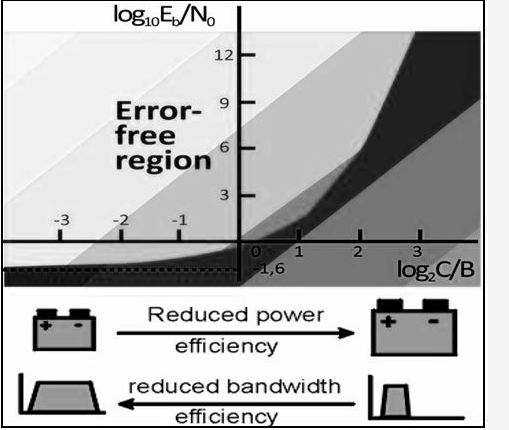
\includegraphics [width=0.75\textwidth]{F/image4.png}
\caption{Shannon–Hartley theorem}
\label{fig:F1}
\end{figure}
 
	The graphical representation of the Shannon–Hartley theorem, see Fig.\ref{fig:F1}, clearly shows that throughput can be traded for power efficiency, and vice-versa. The light gray area represents the area free from errors. The theoretical minimum SNR for an error-free transmission is impossible to reach in practice. The modulation schemes define how close to this theoretical SNRmin the transmission can be. Every modulation scheme is characterized by a minimum SNR that allows the demodulation of the transmitted symbols without errors. Knowing the minimum SNR for every modulation scheme (MS), we can define the minimum Signal Power for every MS for specific levels of noise. The equation that defines the symbol error probability (Ps) for every MS, with respect to SNR is the following \cite{7}:

\begin{equation}
P_{s,M-ary}= (\frac{M-1}{M}) \times erfc(\sqrt{\frac{3}{M^{2}-1} \times \frac{E_{Saver}}{N_{0}}})
\end{equation}

\begin{figure}
\centering
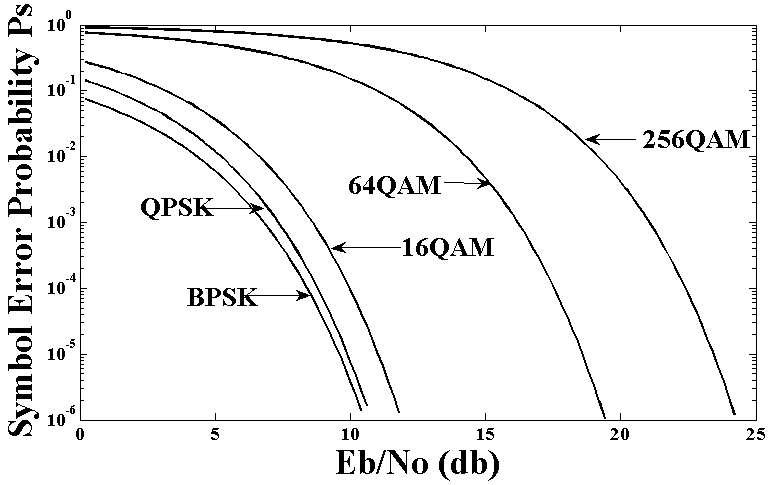
\includegraphics[width=0.75\textwidth]{F/image6.png}
\caption{Symbol error probability for 802.11ac Modulation schemes}
\label{fig:F2}
\end{figure}

\begin{figure}
\centering
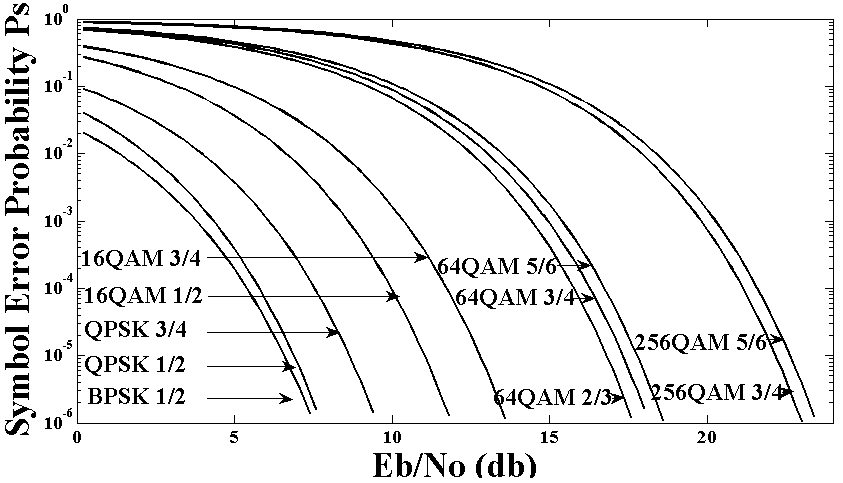
\includegraphics[width=0.75\textwidth]{F/image7.png}
\caption{Symbol error probability for 802.11ac Modulation and Coding schemes}
\label{fig:F3}
\end{figure}

M is the number of symbols used, Es the average received signal power, N0 the average noise signal power and erfc is the complementary error function.
	The graphical expression of this equation for the modulation schemes of the 802.11ac is presented in Fig.\ref{fig:F2}. Channel coding improves the SNR by a factor R \cite{18}. So the curves can be normalized for equal energy per information bit (pre-coding) bearing in mind that the energy per transmitted bit is less than the energy per information bit by a factor equal to the code rate R. The graphical expression of the symbol error probability for the modulation and coding (MC) schemes of the 802.11ac can be found in Fig.\ref{fig:F3}.
	
	In this context, every system scenario RTS is characterized by a two-dimensional cost 1) the total signal power and 2) the bit error rate (BER). The signal power is inversely proportional to the symbol error probability and correspondingly to bit error probability as shown in Fig.\ref{fig:F2} and Fig.\ref{fig:F3}. Each RTS is characterized by a curve in the two-dimensional space of total signal power. This curve is derived by the respective curve at Fig.\ref{fig:F3} that corresponds at the MCs of the RTS. Based on the bits-per-symbol of MCs (BPSK: 1bps, QPSK: 2bps, etc.), the short guard interval (SGI) and the noise level of the RTS, the Ps (symbol error probability) to SNR curve can be transformed to BER to Signal Power curve. In Fig.\ref{fig:F4}, due to limited space, we present 3 representative examples of these RTS curves. For a given BER, the minimum signal power to achieve successful communication is chosen and this point represents the system configuration for this RTS. 
	
\begin{figure}
\centering
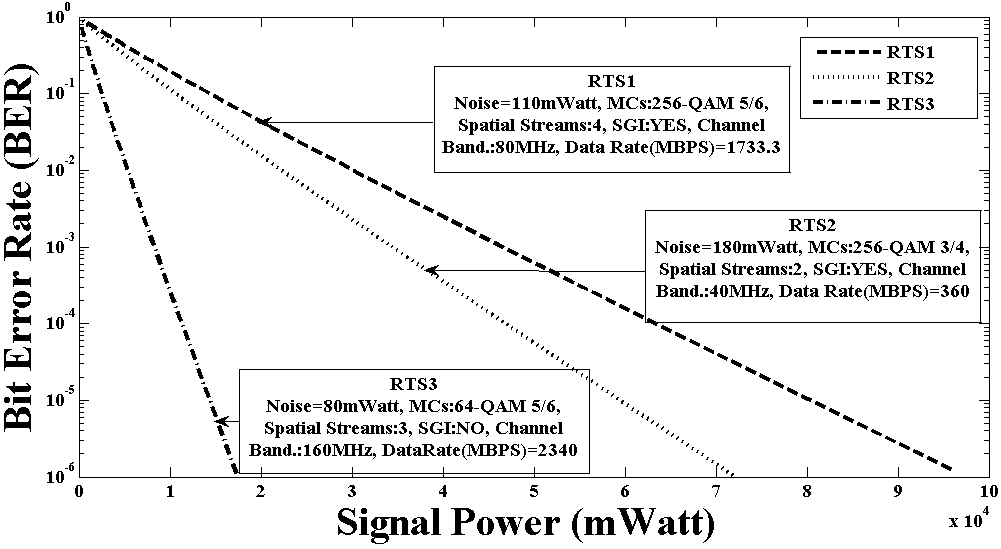
\includegraphics[width=0.75\textwidth]{F/image8.png}
\caption{RTS Characterization}
\label{fig:F4}
\end{figure}	
	
	Besides the above-mentioned technical analysis the most unstable parameter for a transmission is the user profile, e.g., the distance between receiver and transmitter, the existence of other communication channels or others sources of distortion. These are factors that influence the channel transmission and are directly influenced by the user behavior. For example, if the user moves in a saturated spectrum area or in a noisy environment high communication channel interference is expected. Correspondingly, if the user changes position very rapidly, (for example, driving a car) this has impact on the normal demodulation of the transmitted signal (Doppler Effect). 
	
\subsection{Memory Banks}

The SNR level and the changing environment on the wireless channel also affects the memory requirements. In more detail, the conditions of the channel determine the coding and modulation scheme needed for a successful communication and, consequently the required data rate. The coding phase transforms an m-bit data string into an n-bit string in order to be encoded, when the given coding rate is m/n. The modulation phase conveys a varying number of bit streams together, based on the chosen modulation. The data rate constraint defines the storage and transmission requirements for the data. As a result, the memory footprint depends on the data rate of the channel and is dynamic for a changing environment. Energy consumption on the memory subsystem depends on the number of accesses and the energy per access, which are different based on the size and the type of memory.
The observation that the memory requirements at run-time vary significantly due to dynamic variations on the transmission channel and the protocol, is exploited through use of system scenarios. Instead of defining the memory requirements for the worst-case data rate and tuning the system according to this, system scenarios are generated for different situations. The combination of the coding and the modulation parameters define the data rate for each RTS. The data rate is the identification variable and the cost factor is its memory footprint. Based on the cost factor, the different memory footprints are clustered into scenarios. The clustering of RTSs is based both on their distance on the memory size axis and the frequency of their occurrence.

The key feature needed in the platform architecture is the ability to efficiently support different memory sizes that correspond to the system scenarios generated by the methodology. Execution of different system scenarios then leads to different energy costs, as each configuration of the platform results in a specific memory energy consumption. The dynamic memory platform is achieved by organizing the memory area in a varying number of banks that can be switched between different energy states.  

In this work, a clustered memory organization with up to five memory banks of varying sizes is explored. The dynamic memory organization is constructed using commercially available SRAM memory models (MM). For those models delay and energy numbers are derived from a commercial memory compiler. In addition, experimental standard cell-based memories (SCMEM) \cite{19} are considered for smaller memories due to their energy and area efficiency for reasonably small storage capacities. The standard cell-based memories are synthesized using Cadence RTL compiler for TSMC 40nm standard library.

Both MMs and SCMEMs can operate under a wide range of supply voltages, thus support different operating modes that provide an important exploration space. 
\begin{itemize}
\item Active mode: The normal operation mode, in which the memory can be accessed at the maximum supported speed. The supply voltage is 1.1V. The dynamic and leakage power are higher compared to the other modes. In this work all the memory accesses are performed on the active mode.
\item Light/Deep sleep mode: The supply voltage in this mode is lower than active with values around 0.7V and 0.3V respectively. The access time of the memory is significantly higher than the access time in active mode. Switching to active mode can be performed with an energy penalty (switching cost) and a small time penalty of a few clock cycles. Data is retained.
\item Shut down mode: Power-gating techniques are used to achieve near zero leakage power. Stored data is lost. The switch to active mode requires substantially more energy and time. However, switching unused memories to this mode results in substantial energy savings.
\end{itemize}

	The goal is to design a suitable clustered scratchpad memory architecture that can serve the generated scenarios. When the maximum data rate is required by the protocol, all the memory banks should be active and accessed. When the needed data rate is lower, the size and the rate required by the memory system are lower and one or more memory banks can be switched off. As a result, the amount of energy consumed during a system scenario with lower requirements is reduced.
	
\subsection{Combined Model}	

The optimal energy configuration both on the signal power and the memory subsystem takes into consideration six parameters, namely (a) the number of spatial streams (streams), (b) the MC schemes, (c) the channel bandwidth, (d) the SGI, (e) the data rate, and (f) the noise level. Based on their values the run-time manager choses the active scenario for the signal power and the memory subsystem and performs the appropriate reconfigurations. The key point is that this decision is not taken independently. For the first time in the context of a wireless system, two system scenario sets adjusted to achieve an overall optimization. This represents a new methodology extension because the clustering step has to take into consideration not only the overhead impact at the targeted subsystem, but also the interaction with the other subsystem scenario sets. Thus, it is provided an optimal configuration for the whole system and not sub-optimal for individual parts.

\section{Case Study}

In the context of the current case study, we examine the potential power gain exploiting two scenario-based schedulers. The first adjusts dynamically the antenna signal power and the second manages the memory banks activation. For the needs of our study, we consider an artificial application that generates data bursts that have to be transmitted within specific deadlines. The distribution of the generated data bursts is presented at Fig.\ref{fig:F5}. For every data burst there is a corresponding transmission time deadline, which defines a minimum data rate. The distribution of the time deadlines is presented at Fig.\ref{fig:F6}.
 
\begin{figure}
\centering
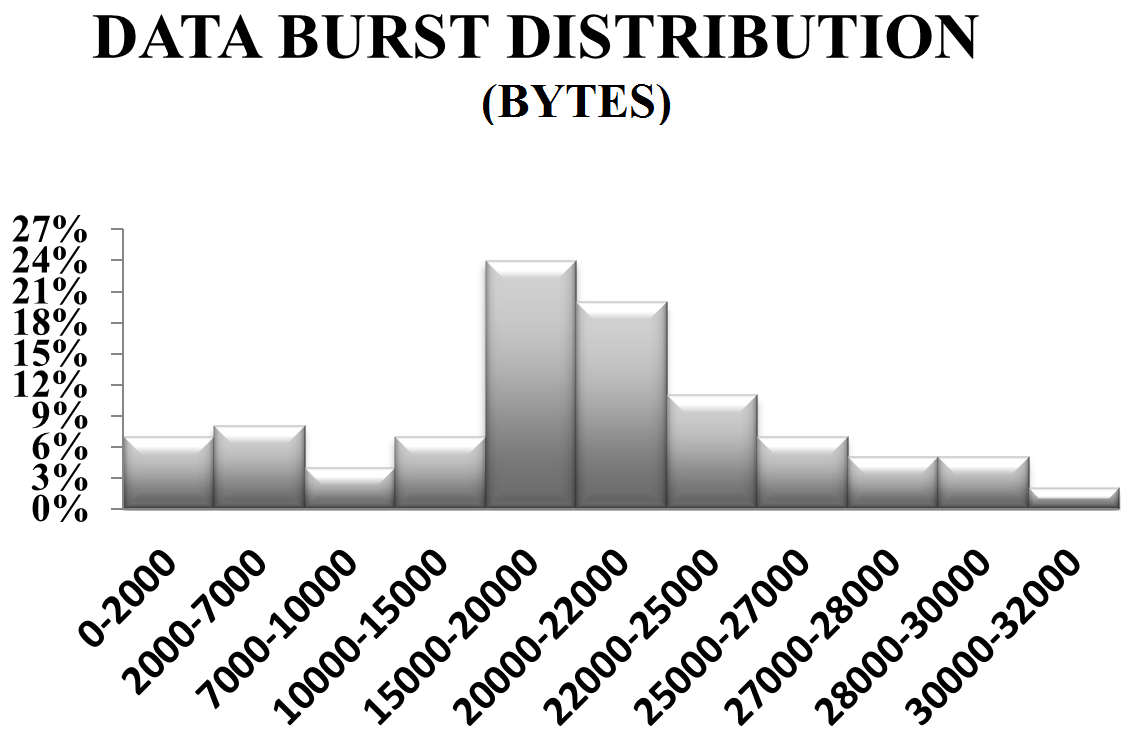
\includegraphics[width=0.75\textwidth]{F/image9.png}
\caption{Data Burst Distribution}
\label{fig:F5}
\end{figure}	

\begin{figure}
\centering
\includegraphics[width=0.75\textwidth]{F/image10.png}
\caption{Application Deadline Distribution}
\label{fig:F6}
\end{figure}	

Every combination of six parameters discussed in Section IV.C represents a different communication scheme. The memory adaptation scheduling takes into consideration only the data rate. The first four parameters (streams, MCs, BW, SGI) is defined by the targeted protocol (802.11ac) \cite{4} creating an exploration space of 240 RTSs. Given values for these four parameters, the maximum value for the fifth parameter, data rate, can be calculated. Thus, data rate does not contribute to the exploration space, but it is used as an identification variable of the suitable communication scheme. More precisely, the desired data rate is extracted dynamically by the running application requirements (Data Bursts size and Deadline) and the scheduler identifies which communication schemes can satisfy this data rate.  
The last and the most important variable is the external noise. In order to be more representative, we take noise distributions and not discrete values of noise.
 For the needs of our measurements we consider two channels with different Gaussian noise distributions as shown in Fig.\ref{fig:F7} having different average values ($\mu$) and standard deviations ($ \sigma $) ($channel_1: \mu  =100mWatt,  \sigma =20mWatt, channel_2:  \mu =140mWatt,  \sigma  = 10mWatt $). 
 The second channel represents a noisier and more rapidly changing environment compared to the first. 
 The noise distribution defines the appearance probability of the running situations (RTSs). 
 A different noise distribution creates a different probability density for the RTSs. For example in our case the probability density of the RTSs, with noise range ($\mu, \mu + \sigma$) and ($\mu$ and $\mu - \sigma$), is 34.13\% (because of the Gaussian distribution). 
 Similarly, the RTSs probability for ($\mu, \mu \pm 2 \sigma$),  ($\mu, \mu \pm 3 \sigma $), ($\mu, \mu \pm 4 \sigma$) and ($\mu, \mu \pm 5 \sigma $) are calculated. 
 Thus, for a Gaussian distribution, we have in total 10 bounding levels of noise, which in combination with the values of the previous parameters creates an exploration space of (240 Χ10) 2400 RTSs. The clustering of the RTSs into system scenarios varies based on the noise distributions. Thus, for every distribution we have a different optimal set of system scenarios.

\begin{figure}
\centering
\includegraphics[width=0.75\textwidth]{F/image11.png}
\caption{Noise Distribution}
\label{fig:F7}
\end{figure}	


The scheduling decision about the suitable communication scheme follows three main priorities: 1) the required data rate, 2) the noise tolerance and 3) the power saving. The first criterion fulfills the current application deadlines while the second ensures the signal power for an acceptable BER. Thus, the signal power scheduler first finds the communication schemes that respect the running time constrain, and in a second stage chooses these, that permit the lowest signal power. The final decision is based on the overall system power saving. 

In our case study, we have in total three different sets of system scenarios; two for the signal power scaling (one for each of the two channels presented in Fig.\ref{fig:F7}) and a third set for the memory banks power management (based on the data size distribution presented in Fig.\ref{fig:F5}). To minimize memory bank power, the memory scheduler at run-time activates a suitable number of scratch pad memory banks based on the selected coding scheme. Data are transferred to the memories as part of the transmission chain during the modulation phase.
	
For the extraction of the system scenarios, we take into consideration the trade-off between the run-time implementation overhead and the accuracy of the extracted scenarios. The first is related to the switching overhead while the second is related to the number of the scenarios and the clustering overhead. In comparison with the approach presented in the second case study of publication \cite{21} (related to signal power adaptation), the presented study has the following differentiations. Except from the different characteristics of protocol 802.11ac (compared with 802.11n), in our case the proposed scheduler both adjusts signal power and selects the optimal power communication scheme (MCs, streams, BW etc.) based on the current noise conditions and data rate constrains. This increases the design space complexity from 80 RTSs \cite{21} to 2400 RTSs. Additionally, the current approach takes into consideration two channel noise distributions (one for every channel) which differentiates the RTS appearance frequency, changing dramatically the clustering of RTSs into system scenarios (as the RTS frequency affects significantly the clustering overhead \cite{21}). Furthermore, in the context of the current study we differentiate by presenting the trade-offs between switching and clustering overhead for different numbers of extracted system scenarios and by including memory into exploration. In respect with the last, we insert a new methodology extension adjusting the clustering of two system scenario sets (Signal Power and memory) to achieve an overall optimization.  
	
\section{Results}

	Tab.\ref{tab:F1}, Tab.\ref{tab:F2} and Tab.\ref{tab:F3} present the variation of the clustering and switching overhead. The first column (number of scenarios) gives the number of system scenarios for each row. The second column (clustering overhead compared to WCE) and third column (clustering overhead compared to previous step) presents normalized the percentage variation of the clustering overhead compared with the worst case (monolithic approach) and that of the previous row, respectively. When RTSs are clustered into scenarios, the cost for the most energy demanding RTS is used as the representative cost for all the RTSs within the scenario. The system is configured to serve the most demanding RTS of the scenario and consequently all the less demanding RTSs, which belong to the scenario. The clustering overhead represents the difference between the RTSs within a scenario. As the number of scenarios increases the percentage approaches 100\%, which would be the value if there was a dedicated scenario for each RTS. Similarly, the fourth column (switching overhead) and fifth column (switching var) represents the switching overhead expressed as the scenario switching probability and the percentage change of the switching overhead compared with that of the previous row, respectively.
	
	In Tab.\ref{tab:F1}, for example, for a set of 8 system scenarios we have a clustering overhead of 7\% and a decrease in clustering overhead compared with the previous row (7 system scenarios) of 19\%. The switching overhead is 85\% and it is increased by 4\% compared with the previous row. For an increasing number of scenarios, the clustering overhead is reduced, because the difference between the RTSs within the scenarios decreases. Respectively, the switching overhead is increased, because there are more scenarios to choose from and thus the system switches between scenarios more often. Depending on the design objectives, it is possible to choose an optimized number of scenarios. A larger number of scenarios increases the implementation overhead (more switching overhead) but it reduces the clustering overhead and vice versa.
	
	The power gain percentages for each of the channels and the memory are presented in Fig.\ref{fig:F8}. Results are given for 10 executions of the case study with the noise distribution given in Fig.\ref{fig:F7}. The baseline is a system designed based on the worst-case requirements. The system is assumed monolithic without any reconfiguration based on the noise level and the MC scheme. The gain for the first antenna is around 97\% for all the cases, while for the second antenna it is a little lower. The worst case has a noise level of 180 mWatt, MC scheme 5/6 256QAM, SGI and 4 MIMO, while best case has a noise level of 20 mWatt, MC scheme 1/2 BPSK, no SGI and 1 MIMO. The reported gains for the memory are in the range from 27.8\% to 29\%. The power savings are significantly higher on the antennas due to two main reasons. Firstly, the variation between the best and the worst case on the antennas is wider and thus offers a greater opportunity for energy savings. Secondly, the reconfiguration option for the antennas offer more flexibility and all possible signal power levels can be exploited. The memory architecture has a physical limitation in the number of memories that can be used and only a range of sizes is supported by the system models.

\begin{table}
\centering
	\caption{Memory Banks Scenario Overhead}
	\label{tab:F1}
	\includegraphics[width=0.75\textwidth]{F/tab1.png}
\end{table} 

\begin{table}
\centering
	\caption{Signal power–Channel 1 Scenario Overhead}
	\label{tab:F2}
	\includegraphics[width=0.75\textwidth]{F/tab2.png}
\end{table} 

\begin{table}
\centering
	\caption{Signal power–Channel 2 Scenario Overhead}
	\label{tab:F3}
	\includegraphics[width=0.75\textwidth]{F/tab3.png}
\end{table} 

\begin{figure}
\centering
\includegraphics[width=\textwidth]{F/image15.png}
\caption{Power Gain}
\label{fig:F8}
\end{figure}	 

\section{Conclusion} 

The scope of this work is to explore the power management options for a transmitting wireless system using system scenarios. The dynamic parameters and the variations during the transmission for the targeted wireless protocol are analyzed. Based on the analysis and the system models, system scenarios are generated for the case study, in order to optimize energy usage. Both the signal power and the memory subsystem are taken into consideration. The results demonstrate the effectiveness of the methodology and illustrate the interesting trade-off between the clustering overhead and the switching cost. 
	
\addcontentsline{toc}{section}{Bibliography}	
\bibliographystyle{plain}
\bibliography{dsd_ref}
	
	


\end{document}